%%%%%%%%%%%%%%%%%%%%%%%%%%%%%%%%%%%%%%%%%%%%%%%%%%%%%%%%%%%%%%%%%%%%%%%%%%%%%%%
%% Descr:       Vorlage für Berichte der DHBW-Karlsruhe
%% Author:      Prof. Dr. Jürgen Vollmer, juergen.vollmer@dhbw-karlsruhe.de
%% $Id: bericht.tex,v 1.24 2018/10/23 09:10:06 vollmer Exp $
%%  -*- coding: utf-8 -*-
%%%%%%%%%%%%%%%%%%%%%%%%%%%%%%%%%%%%%%%%%%%%%%%%%%%%%%%%%%%%%%%%%%%%%%%%%%%%%%%

\documentclass[
   ngerman          % neue deutsche Rechtschreibung
  ,a4paper          % Papiergrösse
% ,twoside          % Zweiseitiger Druck (rechts/links)
% ,10pt             % Schriftgrösse
  ,11pt
% ,12pt
  ,pdftex
%  ,disable         % Todo-Markierungen auschalten
]{report}

% Bitte die Codierung Ihrer Dateien auswählen:
% \usepackage[latin1]{inputenc}    % Für UNIX mit ISO-LATIN-codierten Dateien
% \usepackage[applemac]{inputenc}  % Für Apple Mac
% \usepackage[ansinew]{inputenc}   % Für Microsoft Windows
\usepackage[utf8]{inputenc}        % UTF-8 codierte Dateien
                                   % Dieses Dokument ist unter Unix erstellt, daher
                                   % wird diese Input-Codierung benutzt.
\usepackage[english,ngerman]{babel}
\usepackage{bericht}
\usepackage{subfigure}
\usepackage{amsmath}
\usepackage{blindtext}

%%%%%%%%%%%%%%%%%%%%%%%%%%%%%%%%%%%%%%%%%%%%%%%%%%%%%%%%%%%%%%%%%%%%%%%%%%%%%%%
%% Angaben zur Arbeit
%%%%%%%%%%%%%%%%%%%%%%%%%%%%%%%%%%%%%%%%%%%%%%%%%%%%%%%%%%%%%%%%%%%%%%%%%%%%%%%

\newcommand{\Autor}{Mikka Jenne}
\newcommand{\MatrikelNummer}{2062885}
\newcommand{\Kursbezeichnung}{TINF17B4}

\newcommand{\FirmenName}{cjt Systemsoftware AG}
\newcommand{\FirmenStadt}{Karlsruhe}
\newcommand{\cjtFirmenLogo}{
\includegraphics[width=2.5cm]{cjtFirmenLogo}}

% Falls es kein Firmenlogo gibt:
\newcommand{\FirmenLogoDeckblatt}{}

\newcommand{\BetreuerFirma}{M. Sc. Florian Dunz}
\newcommand{\BetreuerDHBW}{Prof. Dr. Marcus Strand}

%%%%%%%%%%%%%%%%%%%%%%%%%%%%%%%%%%%%%%%%%%%%%%%%%%%%%%%%%%%%%%%%%%%%%%%%%%%%%%%%%%%%%

% Wird auf dem Deckblatt und in der Erklärung benutzt:
%\newcommand{\Was}{Projekt-/Studien-/Bachleorarbeit}
%\newcommand{\Was}{Projektrarbeit}
%\newcommand{\Was}{Studienarbeit}
\newcommand{\Was}{Bachelorarbeit}

%%%%%%%%%%%%%%%%%%%%%%%%%%%%%%%%%%%%%%%%%%%%%%%%%%%%%%%%%%%%%%%%%%%%%%%%%%%%%%%%%%%%%

\newcommand{\Titel}{Konzeption und Umsetzung eines Augmented Reality basierten Assistenzsystems zur Unterstützung industrieller Prozesse}
\newcommand{\AbgabeDatum}{31. August 2020}

\newcommand{\Dauer}{12 Wochen}

% \newcommand{\Abschluss}{Bachelor of Engineering}
\newcommand{\Abschluss}{Bachelor of Science}

\newcommand{\Studiengang}{Informatik}
% \newcommand{\Studiengang}{Informatik / Angewandte Informatik}

\hypersetup{%%
  pdfauthor={\Autor},
  pdftitle={\Titel},
  pdfsubject={\Was}
}

%%%%%%%%%%%%%%%%%%%%%%%%%%%%%%%%%%%%%%%%%%%%%%%%%%%%%%%%%%%%%%%%%%%%%%%%%%%%%%%

% Wenn \includeonly{..} benutzt wird, werden nur diese Kaptitel ausgegeben.
%\includeonly{
 % abk
 %,kapitel1
 %,kapitel2
 %,kapitel3
 %,systementwurf
 %,changelog
%}

%%%%%%%%%%%%%%%%%%%%%%%%%%%%%%%%%%%%%%%%%%%%%%%%%%%%%%%%%%%%%%%%%%%%%%%%%%%%%%%

% Benutzt man das "biblatex"-Paket, dann muß das hier stehen:
% siehe auch die mit BIBLATEX markierten Zeilen in bericht.sty
\bibliography{bericht}

\begin{document}

%%%%%%%%%%%%%%%%%%%%%%%%%%%%%%%%%%%%%%%%%%%%%%%%%%%%%%%%%%%%%%%%%%%%%%%%%%%%%%%%

\begin{titlepage}
\begin{center}
\vspace*{-2cm}
\cjtFirmenLogo
\FirmenLogoDeckblatt\hfill
\includegraphics[width=4cm]{dhbw-logo}\\[2cm]
{\Huge \Titel}\\[1cm]
{\Huge\scshape \Was}\\[1cm]
{\large für die Prüfung zum}\\[0.5cm]
{\Large \Abschluss}\\[0.5cm]
{\large des Studienganges \Studiengang}\\[0.5cm]
{\large an der}\\[0.5cm]
{\large Dualen Hochschule Baden-Württemberg Karlsruhe}\\[0.5cm]
{\large von}\\[0.5cm]
{\large\bfseries \Autor}\\[1cm]
{\large Abgabedatum \AbgabeDatum}
\vfill
\end{center}
\begin{tabular}{l@{\hspace{4cm}}l}
Bearbeitungszeitraum	         & \Dauer 			\\
Matrikelnummer	                 & \MatrikelNummer		\\
Kurs			         & \Kursbezeichnung		\\
Ausbildungsfirma	         & \FirmenName			\\
			         & \FirmenStadt			\\
Betreuer der Ausbildungsfirma	 & \BetreuerFirma		\\
Gutachter der Studienakademie	 & \BetreuerDHBW		\\
\end{tabular}
\end{titlepage}
 
%%%%%%%%%%%%%%%%%%%%%%%%%%%%%%%%%%%%%%%%%%%%%%%%%%%%%%%%%%%%%%%%%%%%%%%%%%%%%%%

%%%%%%%%%%%%%%%%%%%%%%%%%%%%%%%%%%%%%%%%%%%%%%%%%%%%%%%%%%%%%%%%%%%%%%%%%%%%%%%
%% Descr:       Vorlage für Berichte der DHBW-Karlsruhe, Erklärung
%% Author:      Prof. Dr. Jürgen Vollmer, vollmer@dhbw-karlsruhe.de
%% $Id: erklaerung.tex,v 1.11 2020/03/13 14:24:42 vollmer Exp $
%% -*- coding: utf-8 -*-
%%%%%%%%%%%%%%%%%%%%%%%%%%%%%%%%%%%%%%%%%%%%%%%%%%%%%%%%%%%%%%%%%%%%%%%%%%%%%%%

% In Bachelorarbeiten muss eine schriftliche Erklärung abgegeben werden.
% Hierin bestätigen die Studierenden, dass die Bachelorarbeit, etc.
% selbständig verfasst und sämtliche Quellen und Hilfsmittel angegeben sind. Diese Erklärung
% bildet das zweite Blatt der Arbeit. Der Text dieser Erklärung muss auf einer separaten Seite
% wie unten angegeben lauten.

\newpage
\thispagestyle{empty}
\begin{framed}
\begin{center}
\Large\bfseries Erklärung
\end{center}
\medskip
\noindent
% siehe §5(3) der \enquote{Studien- und Prüfungsordnung DHBW Technik} vom 29.\,9.\,2017 und Anhang 1.1.13
Ich versichere hiermit, dass ich meine \Was mit dem Thema:
\enquote{\Titel}
selbstständig verfasst und keine anderen als die angegebenen Quellen und Hilfsmittel benutzt habe. Ich versichere zudem, dass die eingereichte elektronische Fassung mit der gedruckten Fassung übereinstimmt.
\vspace{3cm}
\noindent
\underline{\hspace{4cm}}\hfill\underline{\hspace{6cm}}\\
Ort~~~~~Datum\hfill Unterschrift\hspace{4cm}
\end{framed}

\vfill
\emph{Sofern  vom Dualen Partner ein Sperrvermerk gewünscht wird, ist folgende Formulierung
zu verwenden:}
\begin{framed}
\begin{center}
\Large\bfseries Sperrvermerk
\end{center}
\medskip
\noindent
Der Inhalt dieser Arbeit darf weder als Ganzes noch in Auszügen Personen
außerhalb des Prüfungsprozesses und des Evaluationsverfahrens zugänglich gemacht
werden, sofern keine anderslautende Genehmigung vom Dualen Partner vorliegt.
\end{framed}

%%%%%%%%%%%%%%%%%%%%%%%%%%%%%%%%%%%%%%%%%%%%%%%%%%%%%%%%%%%%%%%%%%%%%%%%%%%%%%%
\endinput
%%%%%%%%%%%%%%%%%%%%%%%%%%%%%%%%%%%%%%%%%%%%%%%%%%%%%%%%%%%%%%%%%%%%%%%%%%%%%%%


%%%%%%%%%%%%%%%%%%%%%%%%%%%%%%%%%%%%%%%%%%%%%%%%%%%%%%%%%%%%%%%%%%%%%%%%%%%%%%%
\selectlanguage{english}
\begin{abstract}
  Augmented Reality is a technology that enables the user to have a visual 
  experience with an enriched world full of virtual objects. The result offers the user a new 
  way of perceiving surroundings as an combination of reality and virtuality.
  \\
  \linebreak
  This bachelor thesis deals with the conception and implementation of an industrial assistance system using augmented reality technology. The 
  environment can be analyzed with the help of the SLAM method in order to be able to place three-dimensional objects virtually as a reference to 
  real objects in space. %The resulting visualizations enables information on the respective objects to be entered in a database and also displayed 
  %on screen.
  The user is able to enter specific informations into the database about each emerging visualization.
  This enables the simplified monitoring of industrial machines.
  \\
  \linebreak
  The concept includes the development of the basic software architecture as well as a generally applicable data model for
  saving the generated data. In order to archieve the best augmented reality experience, existing frameworks such as Google ARCore were used.
  \\
  The created prototype is an standalone system. The architecture is build modular in order to ensure continuous further development.
\end{abstract}
\newpage
\selectlanguage{ngerman}
\begin{abstract}
  Augmented Reality ist eine Technologie, die dem Nutzer ein visuelles 
  Erlebnis mit einer angereicherten Welt voller virtueller Objekte ermöglicht. Sozusagen wird eine Kombination aus Realität und Virtualität geschaffen. Das Resultat 
  bietet dem Benutzer eine neue Art der Wahrnehmung der Gegenwart. %Realitätswahrnehmung.  
  \\ 
  \linebreak
  Diese Bachelorarbeit befasst sich mit der Konzeption und Umsetzung eines industriellen Assistenzsystems unter Verwendung der Augmented Reality Technologie. Dabei soll die Umgebung 
  mit Hilfe des SLAM Verfahrens analysiert werden. Auf dieser Basis können dreidimensionale Objekte als Referenz zu realen Objekten im Raum virtuell platziert werden. 
  Durch die entstehende Visualisierung können Informationen zu den jeweiligen Objekten in eine Datenbank eingetragen und angezeigt werden. Diese Arbeit schafft die Grundlage 
  für die Vereinfachung zum Überwachen von Industriemaschinen. 
  \\ 
  \linebreak
  Zu dem Konzept gehört sowohl die Ausarbeitung der grundlegenden Softwarearchitektur, als auch ein allgemeingültiges Datenmodell zur 
  Persistierung der generierten Daten. Für die bestmögliche Umsetzung der Augmented Reality Experience werden hierzu bereits bestehende Frameworks und Software 
  Development Kits verwendet, darunter Google ARCore. 
  \\ 
  Der entstandene Prototyp ist ein eigenständiges System. Die Architektur ist modular aufgebaut. Damit ist eine stetige Weiterentwicklung gewährleistet.  
\end{abstract}
\newpage
\selectlanguage{ngerman}
%\pagestyle{plain}
\chead{\headmark}
\cfoot{\pagemark}
%\pagestyle{headings}
\pagenumbering{Roman}
\tableofcontents           % Inhaltsverzeichnis hier ausgeben
\listoffigures             % Liste der Abbildungen
%\listoftables              % Liste der Tabellen
\lstlistoflistings         % Liste der Listings
%\listofequations           % Liste der Formeln
% Jetzt kommt der "eigentliche" Text
%%%%%%%%%%%%%%%%%%%%%%%%%%%%%%%%%%%%%%%%%%%%%%%%%%%%%%%%%%%%%%%%%%%%%%%%%%%%%%
%% Descr:       Vorlage für Berichte der DHBW-Karlsruhe, Datei mit Abkürzungen
%% Author:      Prof. Dr. Jürgen Vollmer, vollmer@dhbw-karlsruhe.de
%% $Id: abk.tex,v 1.4 2017/10/06 14:02:03 vollmer Exp $
%% -*- coding: utf-8 -*-
%%%%%%%%%%%%%%%%%%%%%%%%%%%%%%%%%%%%%%%%%%%%%%%%%%%%%%%%%%%%%%%%%%%%%%%%%%%%%%%

\chapter*{Abkürzungsverzeichnis}                   % chapter*{..} -->   keine Nummer, kein "Kapitel"
						         % Nicht ins Inhaltsverzeichnis
% \addcontentsline{toc}{chapter}{Akürzungsverzeichnis}   % Damit das doch ins Inhaltsverzeichnis kommt

% Hier werden die Abkürzungen definiert
\begin{acronym}[DHBW]
  % \acro{Name}{Darstellung der Abkürzung}{Langform der Abkürzung}
 \acro{Abk}[Abk.]{Abkürzung}
 \acro{API}[API]{Application Programming Interface}
 \acro{AR}[AR]{Augmented Reality}
 \acro{DBMS}[DBMS]{Datenbank-Management-System}
 %\acro{ER}[ER]{deutsch erweiterte Realität}
 \acro{EKF}[EKF]{Erweiterter Kalman Filter}
 \acro{ERM}[ERM]{Entity-Relationship-Modell}
 \acro{Fraunhofer IOSB}[IOSB]{Fraunhofer Institut für Optronik, Systemtechnik und Bildauswertung IOSB}
 \acro{GPS}[GPS]{Global Positioning System}
 \acro{HMD}[HMD]{Head-Mounted Display}
 \acro{ICP}[ICP]{Iterativ Closest Point}
 \acro{IMU}[IMU]{Inertial Measurement Unit}
 \acro{INS}[INS]{Inertial Navigation System}
 \acro{IoT}[IoT]{Internet of Things, dt. Internet der Dinge}
 \acro{KIT}[KIT]{Forschungszentrum Karlsruhe}
 \acro{MEMS}[MEMS]{Micro-Electro-Mechanical Systems}
 \acro{MR}[MR]{Mixed Reality}
 \acro{MVC}[MVC]{Model View Controller}
 \acro{SDK}[SDK]{Software Development Kit}
 \acro{SLAM}[SLAM]{Simultanious Localization And Mapping}
 \acro{SQL}[SQL]{Structured Query Language}
 \acro{TOF}[TOF]{Time of flight}
 \acro{UX}[UX]{User-Excperience, dt. Nutzererfahrung und Nutzererlebnis}
 \acro{UC}[UC]{Use Case}
 \acro{UCs}[UCs]{Use Cases}
 \acro{UI}[GUI]{Graphical User Interface, dt. Benutzeroberfläche}
 \acro{VR}[VR]{Virtual Reality}
 \acro{WMR}[WMR]{Windows Mixed Reality}
 % Folgendes benutzen, wenn der Plural einer Abk. benöigt wird
 % \newacroplural{Name}{Darstellung der Abkürzung}{Langform der Abkürzung}
 \newacroplural{Abk}[Abk-en]{Abkürzungen}


 \acro{H2O}[\ensuremath{H_2O}]{Di-Hydrogen-Monoxid}

 % Wenn neicht benutzt, erscheint diese Abk. nicht in der Liste
 \acro{NUA}{Not Used Acronym}
\end{acronym}
              % Abkürzungsverzeichnis
\pagenumbering{arabic}
%%%%%%%%%%%%%%%%%%%%%%%%%%%%%%%%%%%%%%%%%%%%%%%%%%%%%%%%%%%%%%%%%%%%%%%%%%%%%%
%% Descr:       Vorlage für Berichte der DHBW-Karlsruhe, Ein Kapitel
%% Author:      Prof. Dr. Jürgen Vollmer, vollmer@dhbw-karlsruhe.de
%% $Id: kapitel1.tex,v 1.17 2018/10/23 08:58:41 vollmer Exp $
%% -*- coding: utf-8 -*-
%%%%%%%%%%%%%%%%%%%%%%%%%%%%%%%%%%%%%%%%%%%%%%%%%%%%%%%%%%%%%%%%%%%%%%%%%%%%%%%

\chapter{Einleitung}
In diesem Teil der Arbeit wird auf die Motivation des Themas eingegangen. 
Die Aufgabenstellung genau erläutert und sowohl die Ziele als auch der Aufbau der Arbeit dargelegt.
\section{Motivation}
Die herkömmlichen Schaltpläne von Gebäuden, Schaltschränken oder Maschinen werden aus der Historie heraus per Hand auf normales Papier
gezeichnet. Der Elektrotechniker oder gar ein Architekt nimmt Zeit in Anspruch einen solchen Plan detailgetreu und 
nach Maßstab zu zeichnen. Diese Arbeit ist sehr zeitintensiv und preislich sehr teuer. Zudem können handschriftliche Änderungen
das Dokument unübersichtlich machen, bzw. müsste bei jeder Änderung ein neuer Plan ausgefertigt werden. 
\\Aus diesen Gründen wird eine Zeichnung meistens vernachlässigt, wobei es für Zukünftige Arbeiten,
z.B. Sanierungen, Ausbauten o.ä. essentiell ist. Um diesem fatalen Fehler, den Plan zu vermeiden, entgegenzuwirken wurden Ideen und
Vorschläge gesammelt, wie dieser Prozess deutlich einfacher und ressourcenschonender vonstattengehen könnte.
\\
\linebreak
Diese Problemstellung der realen Welt führte dazu diese Aufgabe in Angriff zu nehmen und diesen Prozess zu modernisieren.
Mit dem Gedanken und der Intension der Digitalisierung in der Elektrotechnik wurden Überlegungen getätigt diese Modernisierung
umzusetzen.
\linebreak
\linebreak
Ein motivierender Aspekt dieses Vorgehens ist, dass die auf Papier gezeichneten Dokumente verloren gehen oder physische Schäden erleiden können
und so unbrauchbar werden. Durch die Digitalisierung des Verfahrens sind diese Aspekte ausgeschlossen und sind deutlich vielseitiger.
\linebreak
\linebreak
Im Zeitalter der Industrie 4.0, bei der der Schwerpunkt auf Digitalisierung liegt, war es leicht eine Idee zu generieren die 
standardmäßige Schaltpläne in dem Zeichnungs- und Ausarbeitungsprozess verbessert und ein bekanntest Problem löst.
Sowohl in zeitlicher und kostspieliger Hinsicht als auch die Übersichtlichkeit
solcher Dokumente kann enorm gesteigert werden. Veränderungen keine neue Zeichnung anzufertigen, sondern können in der bestehenden
Datei schnell und einfach ausgebessert werden. 
\newpage
\section{Aufgabenstellung}
Es soll ein Konzept für eine Software erstellt werden, welches erlaubt Schaltpläne digital zu zeichnen, anzuzeigen, 
flexibel zu ändern und alle wichtigen Informationen zu Verfügung zu stellen. 
\\ Dieses ausgearbeitete Konzept soll einen modularen Ansatz verfolgen, um in Zukunft beliebig erweiterbar zu sein
und die Integration von neuen Features zu gewährleisten. Nach Erstellung des Konzepts und der definierten Software-Architektur
soll der Grundbaustein der Applikation gelegt und gefestigt werden, indem die Grundfunktion implementiert und getestet werden.
\\Die Grundfunktionen werden in folgendem kurz aufgelistet, um einen groben Überblick zu verschaffen.
\begin{itemize}
    \item Startmenü - Übersicht
    \begin{itemize}
        \item Erstellen eines Schaltplans
        \item Öffnen einer vorhandenen Schaltplan-Datei
        \item Weiterarbeiten an einer Schaltplan-Datei
    \end{itemize}
    \item Editor
    \begin{itemize}
        \item Grundgerüst Zeichen (Grundriss, Türen, etc.)
        \item Leitungen Zeichen (Größe, Stärke der Leitung)
        \item Mögliche Komponenten einfügen (Steckdose, Lichtschalter, etc.) 
        \item Anzeige von Informationen zu Komponenten und Leitungen
        \item Legende zum Verständnis und zur Übersicht der einzelnen Zeichenkomponenten
    \end{itemize}
    
\end{itemize}
Die obenstehenden Punkte sehen die Grundfunktionen vor und werden in drei große Teilbereiche, wie zu erkennen, abgegrenzt. 
Das Design und der allgemeine Aufbau wird in folgenden Kapiteln genauer erläutert und anhand von Bildern,
Mockups und Diagrammen dargestellt.
\linebreak
\linebreak
Der Hauptaugenmerk dieser Aufgabe, bzw. der Problemstellung liegt darin die Möglichkeit zu schaffen
einen Schaltplan rentabel und einfach zu digitalisieren, um den Einsatz von Schaltplanzeichnungen erneut zu verbreiten beziehungsweise
zu modernisieren. 
\newpage
\section{Aufbau der Arbeit}
Nach den oben genannten einleitenden Informationen widmet sich das Kapitel 2 den essentiellen und wichtigsten Grundlagen dieser Arbeit.
Zu Anfang werden allgemein gültige Grundlagen zur Digitalisierung in der Gebäudetechnik (2.1) offenbart, um Kontexte zur Arbeit im Allgemeinen
zu verstehen, gefolgt von einer Einführung in die modulare Software Architektur (2.2) zum Ende des Kapitels.
\linebreak
\linebreak
Anschließend auf Kapitel 2 wird in Kapitel 3 auf die verwendeten Technologien und Tools eingegangen. Mit Windows Presentation Foundation
(3.1) wird erläutert was es damit auf sich hat und welche Programmiersprache diese Technologie sich zu eigen macht. In (3.2) wird das MVVM-Pattern
genauestens erklärt, was es bedeutet, wie und warum es angewendet wird. Das Windows eigene System.Drawing, welches zum 
Zeichnen der Schaltpläne verwendet wird in (3.3) aufgeführt.
\linebreak
\linebreak
Nach den verwendeten Technologien geht es in Kapitel 4 um den eigentlichen Systementwurf, zum einen um das Architekturkonzept (4.1)
und zum anderen um das Softwarekonzept (4.2). Dabei wird auch detailliert auf das Aussehen eingegangen und die graphischen Benutzeroberflächen, GUIs,
anhand mehreren Mockups dargelegt.
\\
\linebreak
In Kapitel 5 wird genauestens auf die praktische Umsetzung und Implementierung der vier definierten Use Cases eingegangen, 
die im einzelnen kurz chronologisch aufgeführt werden.
\begin{itemize}
    \item Startmenü (5.1)
    \item Toolbox (5.2)
    \item Zeichenfläche (5.3)
\end{itemize}
Die letzten zwei Kapitel, Ereignis (6) und Ausblick (7), runden die Dokumentation ab und schließen die Arbeit. Das Ergebnis wird hierbei
analysiert und Verbesserungsvorschläge angemerkt. 
\\ Der Ausblick gibt Aufschluss darüber welche möglichen Erweiterungsmöglichkeiten es gibt und wie die Zukunft dieser Arbeit möglicherweise aussehen könnte.

%%%%%%%%%%%%%%%%%%%%%%%%%%%%%%%%%%%%%%%%%%%%%%%%%%%%%%%%%%%%%%%%%%%%%%%%%%%%%
%% Descr:       Vorlage für Berichte der DHBW-Karlsruhe, Ein Kapitel
%% Author:      Prof. Dr. Jürgen Vollmer, vollmer@dhbw-karlsruhe.de
%% $Id: kapitel2.tex,v 1.5 2017/10/06 14:02:51 vollmer Exp $
%%  -*- coding: utf-8 -*-
%%%%%%%%%%%%%%%%%%%%%%%%%%%%%%%%%%%%%%%%%%%%%%%%%%%%%%%%%%%%%%%%%%%%%%%%%%%%%%%

\chapter{Grundlagen}
\label{chap:Grundlagen}
In diesem Kapitel werden die für diese Bachelorarbeit notwendigen Grundlagen geschaffen, um ein fundiertes Wissen und Verständnis 
über verwendete Technologien zu schaffen. Auf alle diese Informationen und Voraussetzungen wird im Folgenden eingegangen, um nachfolgende 
Konzeption und Umsetzung besser zu verstehen.

\section{Augmented Reality}
\label{chap:Augmented Reality}
Eine der wichtigsten Grundlagen dieser Arbeit ist das Verständnis des Begriffs der Augmented Reality.
\\ 
\acl{AR}, deutsch erweiterte Realität, ist eine durch den Computer gestützte Erweiterung der Realität, bzw. der menschlichen 
Wahrnehmung. Es ermöglicht dem Nutzer die reale Welt mit Überlagerung oder Zusammensetzung virtueller Objekte und visueller Informationen
zu sehen. Mittels einer Art Overlay werden diese Objekte und Informationen über die reale Welt gelegt und dem Nutzer zur Verfügung gestellt. 
Allgemein soll damit dem Nutzer ein weit gefächerter Überblick verschafft werden und Hilfestellung leisten, aber den Nutzer in keinerlei 
Interaktion mit der Umgebung einschränken. Die Definition, welche sich in der Wissenschaft weitestgehend durchgesetzt und etabliert hat ist 
die Definition nach Azuma aus dem Jahre 1997.
\begin{quote}
    „Augmented Reality (AR) is a variation of Virtual Environments (VE), or Virtual Reality as it is more commonly called. VE 
    technologies completely immerse a user inside a synthetic environment. While immersed, the user cannot see the real world around him. 
    In contrast, AR allows the user to see the real world, with virtual objects superimposed upon or composited with the real world. 
    Therefore, AR supplements reality, rather than completely replacing it.“ \cite{azuma.1997a}
\end{quote}
Ein Augmented Reality System verfügt nach \cite{azuma.1997a} über folgende drei charakteristische Merkmale: 
\begin{enumerate}
    \item Es kombiniert Realität und Virtualität.
    \item Es ist interaktiv in Echtzeit.
    \item Die virtuellen Inhalte sind im 3D registriert.
\end{enumerate}
Das erste genannte Merkmal kombiniert die reale Welt mit dem oben genannten Overlay, der Überlagerung der Realität um künstliche virtuelle 
Objekte und visuelle Informationen. Dies bedeutet, der Nutzer nimmt die reale Umgebung gleichzeitig mit den darin liegenden virtuellen 
Objekten als ein Ganzes wahr. Daraus resultiert die Interaktion von virtuellen Objekten und Informationen mit der realen Welt in Echtzeit, 
damit sie als Teil der Realität registriert werden können. Das dritte Merkmal umfasst die Darstellung von Objekten als scheinbar reales 
Objekt. Mit dem letzt genannten Merkmal wird das Ziel verfolgt die projizierten, bzw. nicht realen Teile täuschend echt in die Umgebung zu 
integrieren.
\\ 
\linebreak  
%Darüber hinaus sind die virtuellen Inhalte in 3D (d. h. geometrisch) registriert. Dies bedeutet nichts anderes, als dass in einer 
%AR-Umgebung ein virtuelles Objekt scheinbar einen festen Platz in Realität hat und diesen, sofern es nicht durch eine Benutzerinteraktion 
%verändert wird oder sich z. B. in Form einer Animation selbst verändert, auch beibehält. Mit anderen Worten: Es verhält sich aus Nutzersicht 
%genauso, wie ein reales Objekt, was sich an diesem Ort befinden würde
Eine etwas allgemein formuliertere Definition ist die nach \cite{springer.2019s}, welche die drei charakteristischen Merkmale besonders 
aufgreift:
\begin{quote}
    „Augmentierte Realität (AR) ist eine (unmittelbare und interaktive) um virtuelle Inhalte (für beliebige Sinne) angereicherte Wahrnehmung der 
    realen Umgebung in Echtzeit, welche sich in ihrer Ausprägung und Anmutung soweit wie möglich an der Realität orientiert, sodass im 
    Extremfall (so dies gewünscht ist) eine Unterscheidung zwischen realen und virtuellen (Sinnes-) Eindrücken nicht mehr möglich ist.„ \cite{springer.2019s}
\end{quote}
Diese Definition nimmt sich als Grundlage die oben aufgeführte Definition nach \cite{azuma.1997a}.
\\ 
\linebreak
Der Author L. Frank Baum \cite{frankbaum.1856m} verkündete die ersten Ideen und Gedanken einer Augmented Reality Anwendung in 
\textit{„The Master Key“} \cite{masterkey.1996f}. Eine erste tatsächliche Realisierung eines Augmented Reality Systems erfolgte erst über 
60 Jahr später. Ivan Edward Sutherland \cite{sutherlandbio.1938m} stellte sein Projekt 1968 an der University of Utah vor. Dabei handelte es 
sich um ein sogenanntes \textit{\ac{HMD}}. Ziel dieser Entwicklung war weniger das Erweitern der Realität, sondern dreidimensionale 
Illusionen zu erzeugen die reale Objekte mit einer einfachen Grafik in Echtzeit überlagert. %\cite{display.1965f}
Trotz dessen gilt er als erste Person mit der Vision, einen Nutzer in realer Umgebung mit virtuellen Objekten interagieren zu lassen.
\\ 
Anfang der 90er Jahre prägten zwei Forscher, Thomas P. Caudell und David W. Mizell, den Begriff der Augmented Reality durch ein Pilotprojekt
bei Boeing. Das Projekt diente dazu Informationen in das Gesichtsfeld über eine Brille einzusetzen, um Arbeitern das Verlegen von Kabeln im und um das 
Flugzeug zu erleichtern. Nach dieser bahnbrechenden Erfindung begann eine stetige Weiterentwicklung der Technologie. Im Jahre 1999 wurde 
von Hirokazu Kato und Mark Billinghurst \textit{ARToolKit}, ein Computer-Vision-basiertes Tracking für AR, veröffentlicht und „löste eine 
große Welle an Forschungsarbeiten auf der ganzen Welt aus.“ \cite{springer.2019s} 
\begin{quote}
    We describe an augmented reality conferencing system which uses the overlay of virtual images on the real world. Remote collaborators 
    are represented on Virtual Monitors which can be freely positioned about a user in space. Users can collaboratively view and interact 
    with virtual objects using a shared virtual whiteboard. This is possible through precise virtual image registration using fast and 
    accurate computer vision techniques and HMD calibration. We propose a method for tracking fiducial markers and a calibration method 
    for optical see-through HMD based on the marker tracking. \cite{artoolkitsheet.1999o}
\end{quote}
Dieser Ausschnitt war der grundlegende Baustein des Durchbruchs dieser Technologie und den vorangestellten Forschungen und eine fundierte 
Grundlage für alle Forschungen und Entwicklungen die darauf folgten. 
\\ 
Heutzutage dreht sich die Entwicklung um mobile AR, welche durch die anfängliche Revolution von \textit{ARToolkit} und die darauf entstehenden 
Entwicklungen und Produktionen von großen Firmen, wie z.B. Google, Microsoft, Apple und Facebook entstand. Die zuletzt große Bewegung in dem 
Bereich der AR waren die Vorstellungen großer Software-Plattformen für mobile \acs{AR}-Applikationen. Durch \textit{Apple's ARKit} und \textit{Google's ARCore} 
kamen im Jahr 2017 zwei moderne und innovative Frameworks auf den Markt, die die Entwicklung von \acl{AR}-Applikationen stark beeinflussen.
Die Frameworks wurden bei den ersten Produktionen für Entertainment-Anwendungen genutzt, um z.B. mobile Spiele zur Unterhaltung oder 
Funktionen bei Sport-Fernsehübertragungen zur Anzeige der Entfernung des Freistoßes zu realisieren.
\\ 
\linebreak
Diese Arbeit jedoch widmet sich ausschließlich dem industriellen Aspekt und stellt andere Bereiche in den Hintergrund. Die in Kapitel 
\ref{chap:Motivation} aufgeführte Markstudie bestätigt das enorme Potential hinter \acl{AR} und deren Einsetzbarkeit in der Industrie.
Hauptsächlich in der Produktion, der Wartung oder der Reparatur von Maschinen kann Augmentierte Realität eingesetzt werden und zeigt einen 
positiv erzeugten Mehrwert. Dabei können bei Maschinen das Anzeigen von protokollierten Fehlern oder eine visuelle Hilfestellung bei Defekts, sowohl bei der 
Reparatur, als auch bei der Ersetzung einzelner Komponenten eine deutliche Reduzierung des zeitlichen Aufwands oder eine effektivere Arbeitsweise 
vorweisen. 
\\
\textit{Harvard Business Review} legte einen Vergleich offen, indem ein Techniker ein Steuergerät einer Windkraftanlage mithilfe 
eines \acs{AR}-Headsets verkabelt und in Betrieb nimmt. Alle benötigten Informationen wurden Schritt für Schritt über das Headset zur Verfügung 
gestellt. Dadurch gab es keinen Mehraufwand, z.B. das Nachschlagen in einer Dokumentation. Danach führte der Techniker den gleichen Prozess 
ohne die Hilfe der AR-Anwendung durch, lediglich mit Verwendung des vorliegenden Handbuchs, welches physisch beiseite lag.
Dieser Test bestätigte eine Leistungsverbesserung des Arbeiters beim ersten Gebrauch um \textit{34\%}.\cite{harvardbr.2017m} Diese Erkenntnis 
des Tests stützte den Gedanken der Leistungsverbesserung und der Reduzierung des zeitlichen Aufwands, somit lies dieses Resultat den 
Anlass zu dieses Ergebnis auf die Gesamtheit zu projizieren und für alle Anwendungsfälle allgemeingültig zu machen. 

% https://ntrs.nasa.gov/search.jsp?R=19830003536 
% https://ntrs.nasa.gov/archive/nasa/casi.ntrs.nasa.gov/19830003536.pdf 
% https://www.arsoft-company.com/en/dar-project/

\subsection{Virtual Reality, Augmented Reality und Mixed Reality}
Während immer mehr Leute mit dem Begriff Virtual Reality etwas anfangen können, gibt es doch noch viele Unsicherheiten bei den dazukommenden 
Begriffen der Augmented und der Mixed Reality. Diese drei Begriffe lassen sich meist nicht immer voneinander unterscheiden, da es viele 
Überschneidungen aber auch gravierende Unterschiede gibt. 
\\ 
Folgender Abschnitt beleuchtet die Unterschiede und lässt die drei Formen der erweiterten Realität voneinander unterscheidbar machen.
\subsection*{Virtual Reality}
Virtual Reality, dt. Virtuelle Realität (\acs{VR}), ist eine in Echtzeit computergenerierte, interaktive und virtuelle Umgebung. Eine Darstellung 
und gleichzeitige Wahrnehmung der Wirklichkeit in all ihren Facetten und Eigenschaften. Das Ziel dieser Technologie ist, den Nutzer von der 
Außenwelt abzuschirmen und diese durch eine computergenerierte und detaillierte Welt zu ersetzen. \cite{vr.2018n} Auch bekannt als Immersion.
\\ 
\linebreak
Die konventionelle Computergraphik ist für den Menschen spürbar nicht von belangen und weckt keine physischen Emotionen, wogegen VR diese 
etwas beeinflussen kann. Wie diese Unterschiede spürbar sind, wird in folgendem erläutert.
\\  
Die Tabelle \ref{tbl:vrtabelle} fasst die Unterscheidungsmerkmale von Virtueller Realität zur konventionellen Computergraphik zusammen. \cite{springer.2019s}
\begin{table}[!htb]
    \centering
    \begin{tabular}{ll}
      \textbf{3D- Computergraphik}  & \textbf{Virtuelle Realität} \\
      \hline
      Rein visuelle Präsentation & Multimodale Präsentation \\ %(d. h. mehrere Sinnesmodalitäten ansprechende also z. B. gleichzeitig visuelle, akustische und haptische)
      \hline
      Präsentation nicht notwendigerweise zeitkritisch & Echtzeitdarstellung \\
      \hline
      Exozentrische Perspektive & Egozentrische Perspektive \\
      \hline
      Statische Szene oder vorberechnete Animation & Echtzeitinteraktion und -simulation \\ 
      \hline
      2D-Interaktion (Maus, Tastatur) & 3D-Interaktion (Körperbewegung, -gestik) \\ 
      \hline
      Nicht-immersive Präsentation & Immersive Präsentation \\ 
    \end{tabular}
    \caption{Merkmale der Computergraphik gegenüber der VR \cite{springer.2019s}}
    \label{tbl:vrtabelle}
    % Verweis im Text mittels \ref{tbl:vrtabelle}
\end{table}
\\ 
\linebreak 
Virtuelle Realität ist immer in Verbindung mit \acl{HMD}s zu betrachten, da ein Gerät benötigt wird, welches den Nutzer von der realen Welt 
abschottet und in die virtuelle Welt begleitet. Diese werden auf Hochtouren von großen Firmen, wie Microsoft, Sony, Facebook etc. entwickelt. 
Die erste entwickelte und auf dem Markt veröffentlichte Brille war die HoloLens von Microsoft, gefolgt von der Brille Namens Oculus Rift von 
Facebook usw. 
\\ 
Mit der stetigen Weiterentwicklung dieser Brillen und der Technologie wird versucht nach und nach mehr Sinne des Menschen manipulieren zu 
können, bzw. das Spiel- und Gefühlserlebnis bei Konsolen-Spielen immer realistischer zu gestalten. Allerdings sind die Möglichkeiten im 
Massenmarkt stark beschränkt auf die folgenden aufgelisteten Sinne: 
\begin{itemize}
    \item Sehen: Durch \acl{HMD}s (Oculus Rift), die die reale Welt abschirmen und vom Nutzer nicht mehr wahrgenommen werden kann
    \item Hören: Durch Kopfhörer, somit werden Geräusche der Realität übertönt 
    \item Fühlen: Durch Controller mit haptischem Feedback, um Ereignisse der virtuellen Welt physisch spürbar zu gestalten. 
\end{itemize}
Die Entwicklung dieser Technologie wird uns in Zukunft weiter verfolgen. Vielleicht gibt es irgendwann die Möglichkeit weitere Sinne virtuell 
zu steuern. An den Universitäten von Singapur und Tokio zum Beispiel, gibt es Forscher-Teams die ein großes Budget zur Verfügung haben, um 
dieser Sinnestrübung auf den Grund zu gehen. Sie fanden heraus, das thermische und elektrische Stimulationen bestimmte Geschmackseindrücke 
vermitteln können. Auch Wissenschaftler in China und an der Oxford University haben herausgefunden, dass bestimme Audiosignale mit einem süßen 
Geschmack assoziiert werden. \cite{sinnesforschung.2017m} Forscher aus aller Welt gehen mit einer bestimmten Ernsthaftigkeit die Möglichkeiten 
der Sinneserweiterung in der virtuellen Realität an.   
\subsection*{Augmented Reality}
\ac{AR} setzt im Gegenzug zu \ac{VR} auf das tatsächliche Erweitern der Realität durch das Einblenden von Informationen, Vorgängen, Hilfestellungen
oder die Wegbeschreibung bei Head-Up Displays in Personen-, Kraft- und Nutzfahrzeugen, während \acl{VR} den Nutzer in eine völlig eigene 
Welt entlockt und von der Realität abkapselt. Bei \acs{AR} soll dem Nutzer die zu bewältigenden Aufgaben und dessen Bestreben vereinfacht und 
gestützt werden ohne die Realität außer Acht zu lassen. Darüberhinaus bietet \acl{AR} deutlich mehr Ansatzmöglichkeiten diese Technologie 
umzusetzen und zu nutzen, z.B. wie erwähnt durch Head-Up Displays bei Autos und Flugzeugen, durch Smartphones und Tablets die durch die Kamera 
die Realität erweitern, Brillen mit eingeblendeten Projektionen, wie die Oculus Rift und anderweitige große Projektionen. 
\\ 
In Kapitel \ref{subchap:Varianten der AR} wird auf die Varianten genauer eingegangen. 

\subsection*{Mixed Reality}
Dem Namen entsprechend ist \ac{MR} eine Mischung aus \acl{AR} und \acl{VR}, jedoch die Art und Weise ist dabei entscheidend. Es gibt \acs{MR}
-Brillen, die die reale Welt als Basis der Interaktion nehmen und Brillen die alleinig auf digitalen Bildern aufbauen. \cite{mr.2018o}
\subsubsection*{Mixed Reality bezüglich der realen Welt}
Diese Art der erweiterten Realität basiert auf den gegebenen Grundlagen der \acs{AR}. Ähnlich zu \acl{AR} werden Objekte der realen Welt 
hinzugefügt, indem sie an bestimmte Stellen projiziert werden. \acl{MR} baut darauf auf und verankert die digitalen Objekte mit dem realen
dreidimensionalen Raum, sodass eine Realitätsnahe Interaktion stattfinden kann. Virtuelle und echte Welt verschmelzen dadurch endgültig zu 
einer einzigen Welt. 

\subsubsection*{Mixed Reality bezüglich der virtuellen Welt}
Hinsichtlich der \acs{VR} gibt es zu Anfang keine grundlegenden Änderungen gegenüber der \acs{MR}. Hierbei kann der Nutzer durch 
\acs{MR} ebenso die Außenwelt ausblenden und sich lediglich auf die virtuelle Wahrnehmung fixieren. Erst in der Benutzung werden die Unterschiede 
zu \acs{VR} sichtlich und dieser ist gravierend. Der Nutzer kann sich frei bewegen, d.h. die Bewegungsfreiheit wird nur durch die reale Umgebung 
eingeschränkt, während \acl{VR} sich auf einen sensorgestützten Raum begrenzt. \cite{vr.2018n}
\\ 
Bei \acs{MR} wird jeder Schritt und jede Bewegung in die computergenerierte Welt übertragen und schafft so deutlich mehr Bewegungsfreiheiten.
\\ 
\linebreak 
Ein großer Investor dieser Technologie ist Microsoft mit \ac{WMR}, wobei bereits schon Erfolge erzielt werden konnten. Eine Standhafte Plattform 
die nur darauf wartet ausgebaut und intensiver genutzt zu werden. Für die Plattform vorgesehene Brillen gibt es schon viele Produzenten, wie z.B. 
die \textit{HMD Odyssey} von Samsung oder der \textit{Explorer} von Lenovo.

\subsection{Varianten der Augmented Reality}
\label{subchap:Varianten der AR}
Augmented Reality Anwendungen funktionieren alle nach dem gleichen Prinzip und verfolgen das gleiche Ziel, die Realität durch digitale Informationen 
oder Objekte zu erweitern. Die einzige deutliche Abweichung ist das jeweilige Endgerät und die technische Umsetzung in Zusammenhang mit der 
Hardware. Auf zwei dieser Varianten, mobiles und Smart-Brillen- oder auch Headset-AR genannt, wird in Folgendem eingegangen.

\subsection*{Mobiles AR}
Smartphones sind in unserer Gesellschaft nicht mehr wegzudenken und haben sich fest etabliert. Durch die vielseitige und alltägliche Nutzung 
von Tablets und Smartphones eröffnete diese Sparte eine gute Möglichkeit \acl{AR} in den Alltag zu integrieren. Somit beleibt der ständige 
Gebrauch dieser Technologie nicht aus und bereichert die Art und Weise Spiele und Anwendungen zu entwickeln und zeigt den Fortschritt der technologischen 
Aspekte sowohl software-, als auch hardware-technisch.
Durch die im Smartphone integrierte Kamera werden Live-Aufnahmen analysiert und dienen als Ausgangssituation für die \acs{AR}-Anwendung. Durch 
die gegebene Möglichkeit der vorhandenen Kamera, kann ein Echtzeithintergrund erzeugt und zusätzlich mit Informationen per Overlay dargestellt 
werden. Je nach Anwendung kann der Nutzer auf verschiedene Weise mit den eingeblendeten und virtuellen Objekten interagieren, z.B. durch das 
Bewegen des Geräts, um das Objekt aus verschiedenen Blickwinkeln anschauen zu können, oder der direkten Interaktion mit dem Objekt durch 
Drehen, Skalieren oder Verschieben am Bildschirm. Ein Vorreiter der mobilen AR ist das 2016 auf dem Markt erschienenen \textit{Pokémon Go} 
von Niantic, das den Ansatz der \acs{AR} prägt. \cite{pokemongo.2016a}
\\ 
\linebreak
Die weit verbreitete social Media Applikation \textit{Snapchat} baut seit geraumer Zeit ebenso auf \acl{AR}, um Bilder lebhafter zu 
gestalten, wie der folgenden Abbildung \ref{pic:snapchatAR} zu entnehmen ist. 
\\ 
\linebreak 
\begin{figure}[hbt!]
    \centering
    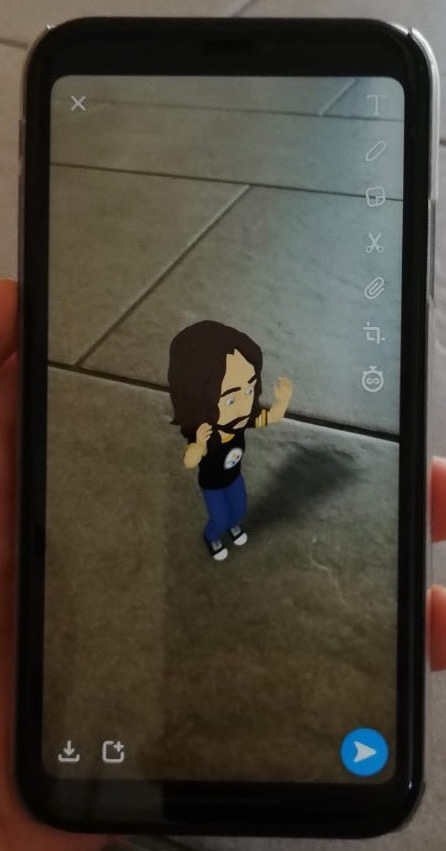
\includegraphics[width=10cm,height=7.5cm,keepaspectratio]{2Grundlagen/Bilder/snapchatAR.jpeg}
    \caption{Mobile-AR in Snapchat}
    \label{pic:snapchatAR}
\end{figure}
\subsection*{Smart-Brillen AR}
Unter Smart- oder Datenbrillen und Smart Glasses wird ein Konstrukt verstanden, das eine Brille mit einem tragbaren Minicomputer verwirklicht. 
Dabei werden Informationen über kleinste Monitore oder Prismen ausgegeben und dem Nutzer zusätzlich in das Sichtfeld projiziert. Im Gegensatz
zur mobilen \acs{AR} hat der Nutzer kein Gerät in der Hand und ist somit in seiner Bewegung weniger eingeschränkt und flexibler. 
\\ 
\linebreak
Die Technologie der Smart-Brillen ist ein ähnliches Konzept zu der \acs{VR}-Brille, allerdings befindet sich die Smart-Brille für den 
öffentlichen Gebrauch noch in der Entwicklungsphase, da nur bedingte Funktionen möglich sind und die Kosten für den Normalverbraucher nur 
bedingt tragbar erscheinen. Mit der überarbeiteten Version der \textit{HoloLens 2} von Microsoft ist eine deutlich komfortablere 
Möglichkeiten des alltäglichen Gebrauchs geboten, da diese im Vergleich zum Vorgängermodell deutlich komfortabler, leichter und 
handlicher ist. Das Design der Datenbrille ist von einer normalen Brille noch weit entfernt, ermöglicht mittlerweile aber das 
uneingeschränkte Sehen und Wahrnehmen der Umgebung. Die Bedienung des Geräts basiert auf schon vorhandenen Möglichkeiten die bereits in anderen 
Geräten Anwendung finden. Darunter gibt es am Gerät angebrachte Touchsensoren, Handbewegungen und -gesten und Eye-Tracking. 
\begin{figure}[hbt!]
    \centering
    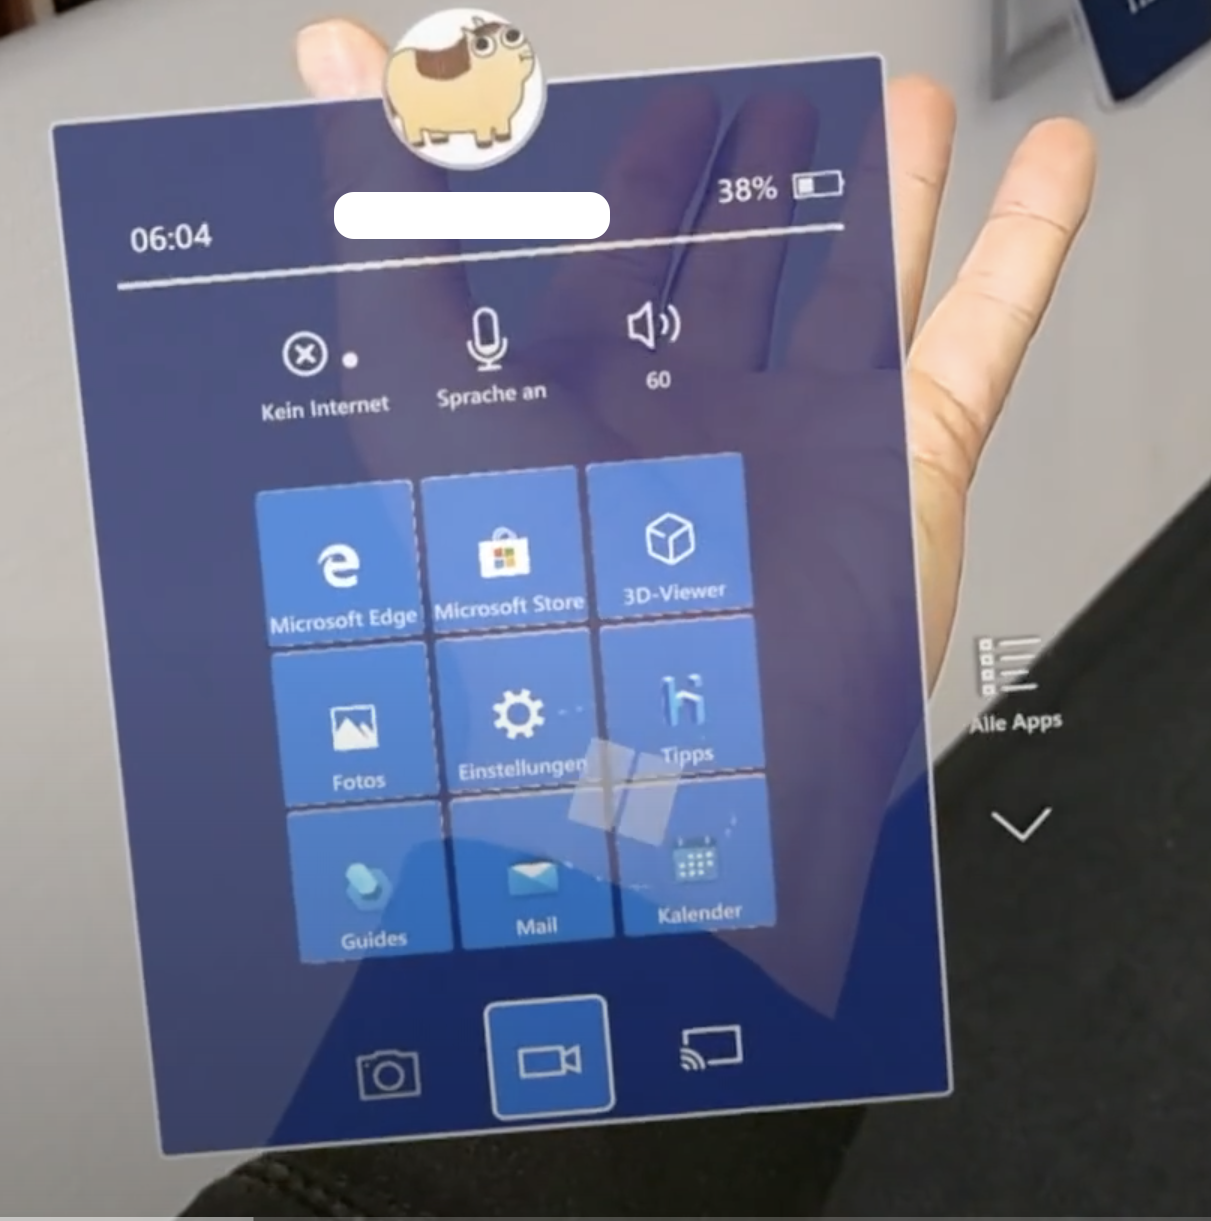
\includegraphics[width=10cm,height=7.5cm,keepaspectratio]{2Grundlagen/Bilder/smartglassAW.png}
    \caption{Test der HoloLens 2}
    \label{pic:testholo}
\end{figure}
\\ 
\linebreak 
Speziell im industriellen Bezug bieten die neuentwickelten Brillen ein komfortables und akzeptables Gewicht, sodass diese ohne große 
Probleme dauerhaft tragbar sind und den Mitarbeiter bei seiner Arbeit nicht übermäßig einschränken.
\\ 
\linebreak
Die Programmierung solcher \acs{AR}-Brillen laufen häufig über eigene \acs{SDK}s und plattformunabhängige Laufzeit- und 
Entwicklungsumgebungen, z.B. Unity oder Unreal Engine. Diese gelten als führende Produkte im Bereich der 3D-Echtzeitdarstellung.
Ein marktführendes Produkt ist unter anderem die Microsoft HoloLens 2, die der folgenden Abbildung zu entnehmen ist. 
\begin{figure}[hbt!]
    \centering
    \subfigure[Google Glass 2]{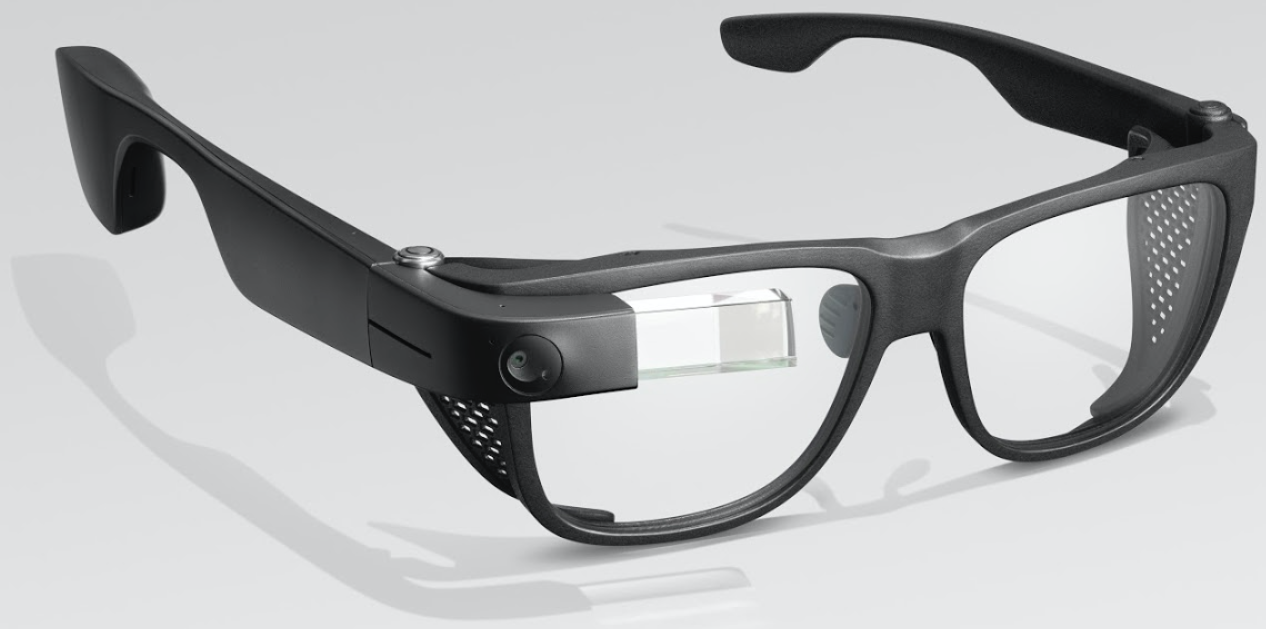
\includegraphics[width=7.5cm,height=5cm,keepaspectratio]{2Grundlagen/Bilder/googleglass.png}}
    \subfigure[HoloLens 2]{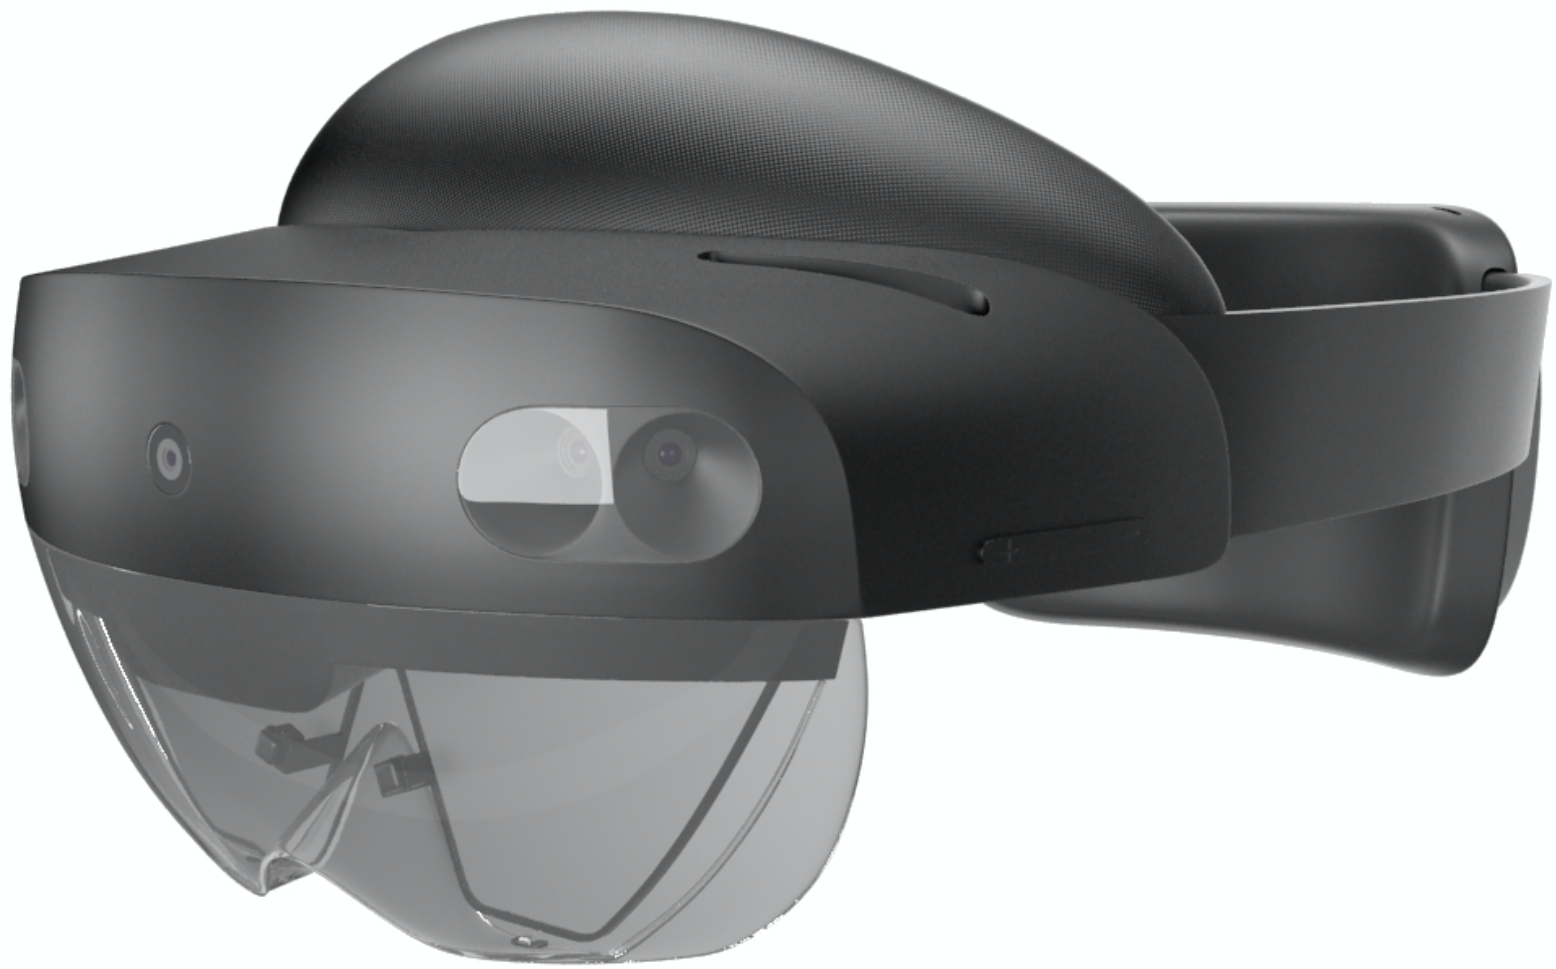
\includegraphics[width=7.5cm,height=5cm,keepaspectratio]{2Grundlagen/Bilder/hololensside.png}}
    \caption{Datenbrillen (\acs{HMD})}
    \label{pic:datenbrillen}
\end{figure}
\\ 
\linebreak
Eine schwer zu umgehende Herausforderung der \acl{AR} ist die Bestimmung der Position in der Daten und Objekte projiziert werden. Auf die 
Ansätze, diese Herausforderung zu bewältigen, wird in folgendem Abschnitt \ref{sec:posi} eingegangen.
\subsection{Positionsbestimmung}
\label{sec:posi}
Um ein digitales Objekt als Overlay dem Kamera-Live-Bild hinzuzufügen, werden genauestens definierte Positionen benötigt. Diese Positionen 
können durch unterschiedliche Ansätze ermittelt werden. Je nach Anwendungsfall, z.B. als Navigation, Routenplaner oder Google Maps 
\textit{„Live View“} \cite{googleliveview.2019a}, reicht eine etwas ungenauere Positionsbestimmung per \acs{GPS}, da in Relation zur 
realen Welt eine Abweichung um Zentimeter oder wenige Meter nicht von belangen ist. Bei Positionsbestimmungen auf kleinstem Raum ist eine 
genaue Lokation wichtig und basiert auf einem deutlich präziseren Ansatz. 
\\ 
Welche oben genannten Ansätze es gibt und welche Unterschiede zu beachten sind, wird in Folgendem näher darauf eingegangen. 
\subsubsection*{Marker-basierte Positionsbestimmung}
Speziell bei der Marker-basierten Positionsbestimmung gibt es verschiedene Möglichkeiten den Marker zu gestalten. Es können 
Binär- oder QR-Codes als Markierung verwendet werden, ein Beispiel eines solchen Codes ist der Abbildung \ref{pic:markerARpos} zu entnehmen. 
Diese Codes sind meistens quadratisch und haben ein eindeutiges Zeichen in der Mitte. Um die Rechenzeit gering zu halten gibt es einfache Muster, 
wie die Abbildung \ref{pic:markerARpos} zeigt.
\begin{figure}[hbt!]
    \centering
    
\includegraphics[width=5cm,height=5cm,keepaspectratio]{2Grundlagen/Bilder/bildmarkerAR.png}
    \caption{Marker-basierte Augmented Reality Positionsbestimmung}
    \label{pic:markerARpos}
\end{figure}
Neben der einfachen Markierungserkennung gibt es eine weiterentwickelte Möglichkeit der Bild- sowie der Objekterkennung. Diese sind Ansätze 
die grundlegend auf dem Ausgangspunkt des Binär-Code-Verfahrens aufbauen. Eine detailliertere Erläuterung der soeben genannten 
Erkennungsmöglichkeiten findet im Rahmen dieser Arbeit nicht statt. Allerdings wird allgemein kurz auf die Funktionsweise einer 
Marker-basierten Positionsbestimmung eingegangen.
\\ 
Durch ein Kamerabild wird nach einem vordefinierten Marker, bzw. nach einer festgelegten Markierung gesucht. Ist diese mit der Kamera erfasst, 
wird die Markierung durch Bildverarbeitungsalgorithmen und bestimmter Filterung eindeutig identifiziert. Mit den gewonnen Informationen und 
der Übereinstimmung des angegebenen Codes wird die Position, sowie die Orientierung des Markers berechnet. Mit den Angaben der Lage und 
Orientierung wird auf der Markierung das anzuzeigende digitale Objekt generiert und als Overlay über dem Kamerabild angezeigt. Die Markierung 
dient sozusagen als Grundlage um den digitalen Gegenstand überhaupt anzeigen zu können.
\\ 
Da der Marker immer im Blickfeld der Kamera sein muss, um das virtuelle Objekt anzuzeigen, bringt diese Art der Positionsbestimmung eine 
enorme Einschränkung mit sich, die in diesem Bezug unumgänglich ist. 
\\ 
\linebreak
Ein weiterer Ansatz der Positionsbestimmung ist als Überbegriff das Gegenstück zur oben aufgeführten Lokalisierung von Markern, die 
sogenannte Marker-unabhängige Positionsbestimmung, welche ebenso verschiedene Ausführungen vorweist. 
\subsubsection*{\acs{GPS}-basierte Positionsbestimmung}
Die Methode des \acs{GPS}-basierten Positionsbestimmungsverfahren verwendet hauptsächlich die Koordinaten der realen Welt. In Zusammenarbeit 
mit zusätzlichen im Anwendungsgerät verbauten internen Sensoren, bspw. Positions-, Geschwindigkeits- und Beschleunigungssensoren und Teile des 
\ac{INS}, z.B. dem Gyroskop, kann diese Art der Positionsbestimmung optimal Anwendung finden. Allerdings werden dabei deutlich mehr Komponenten
benötigt und ist deutlich komplexer umzusetzen, als ein markerbasiertes System. 
\\ 
Bei einem Anwendungsfall von \acs{GPS}-basierter Positionsbestimmung geht es meist um Routenplaner, Navigation oder Szenarien die sich 
auf offenen Flächen abspielen, da im Gegensatz zu Marker-basierten Anwendungen das Größenverhältnis deutlich geräumiger ist. Der Benutzer ist 
nicht auf einen bestimmten Bezirk beschränkt und ist nicht auf die millimetergenauer Darstellung angewiesen.
\\ 
\linebreak
Eine Alternative zu \acs{GPS} ist die Anwendung des \acs{SLAM}-Verfahrens. Dabei wird eine virtuelle Karte, bzw. ein geometrischen Modell der 
Umgebung erstellt. Wichtige Grundlagen zum Erzeugen eines solchen Modells sind eigenständig gefundene Landmarken die gleichzeitig 
lokalisiert werden. Darauf folgt ein Vergleich der Pose, der Position des Geräts und der geschätzten Karteninformationen aus dem Scan der 
Umgebung. 
Damit sind im erweiterten Sinne Marker geschaffen, die Anhaltspunkte für \acl{AR}-Interaktionen schaffen.
\\ 
In Kapitel \ref{chap:SLAM} wird die Thematik des \acs{SLAM}-Verfahrens genauestens erläutert. 

\subsection{Augmented Reality in der Industrie}
Das weit gefächerte Portfolio der \acl{AR} umfasst viele Anwendungsbereiche und Fachgebiete. Selbst dem übergeordneten Bereich der Industrie 
gibt es viele verschiedene Einsatzgebiete. Aus den vielen Möglichkeiten der Anwendung haben sich über die Jahre der Entwicklung der Technologie 
einige Gebiete in der Industrie herauskristallisiert, die besonders hohen Nutzen stiften. \cite{einsatzgebietear.2017a} In den Bereichen 
Instandhaltung und Wartung, Betrieb und Training ist \acl{AR} auf bestem Wege fester Bestandteil des Alltags zu werden. Bei dieser Betrachtung 
ist es sinnvoll sich auf die damit einhergehenden Lösungen zu fokussieren, die Reduktion der Kosten und dem Zeitaufwand, sowie die Verbesserung 
der Sicherheit. \cite{studieptc.2020j} 
\\ 
\linebreak
Bei einer Wartung oder Reparatur einer Maschine sind notwendige Informationen direkt greifbar und werden Schritt für Schritt angezeigt, sodass 
in bestimmten Situationen selbst ein Leihe die Anweisungen befolgen könnte. So werden zusätzliche Recherchearbeiten oder Unklarheiten über 
Vorgänge aus dem Weg geräumt. Ein Mitarbeiter kann so mit einem Tablet oder einer Smart-Glas Anweisungen visuell auf die realen Maschinen 
projizieren und Arbeitsschritte im Sichtfeld anzeigen lassen. Ebenso geht dieser Vorgang auch bei der Produktion von Bauteilen o.ä., indem 
eine \acs{AR}-Anwendung Anweisungen und Prozessschritte, z.B. auf das Werkstück oder Produkt, projiziert.
\\ 
Die Inbetriebnahme oder Bedienung einer komplexen Anlage oder Maschine ist nach herkömmlichen Standard enorm zeitintensiv und dadurch können
zusätzlich viele Fragen aufkommen, die meist den Prozess noch länger gestalten als vorgesehen. \acs{AR}-Anwendungen können 
Bedienungsanleitung oder -hilfen digitalisiert, indem Informationen, Inhalte oder Bedienelemente durch \acl{AR} auf der Anlage platziert werden. 
\\ 
In Fortbildungen, Schulungen oder Einarbeitungen in neue Geräte kann \acs{AR} durchaus von großem Vorteil sein. Mit wenig Aufwand, einem 
effektiveren Training können Schulungen interaktiver und vor allem sicherer abgehalten werden. Durch die Visualisierung der Trainings- und 
Schulungsinhalten verbessert sich der Lernprozess und damit wird auch die Nutzung der Maschinen verständlicher. \cite{einsatzgebietear.2017a}

\section{SLAM - Simultanious Localization And Mapping}
\label{chap:SLAM}
Als Simultaneous Localization and Mapping auch \acs{SLAM}-Problem gennant, bezeichnet man die Aufgabe, die Trajektorie \footnote{Lösungskurve oder Bewegungspfad eines Objekts} 
samt Orientierungsinformation einer sich bewegenden Plattform, z.B. ein Smartphone, Tablet oder jegliche Art von Roboter, aus 
Beobachtungen zu schätzen und gleichzeitig aus den gewonnenen Informationen eine Karte der Umgebung zu erstellen.
Diese Aufgabe ist für den weiteren Prozess von hoher Bedeutung. Zum einen sollen die generierten Karten sehr präzise sein, um einen hohen 
Wert für den Nutzer oder für spezielle Anwendungen, die auf der Karte aufbauen, darzustellen. Zum anderen benötigen autonome Roboter, 
beispielsweise Saug- oder Mähroboter, ein solch erzeugtes geometrisches Modell der Umgebung, um zielgerichtet selbstständig navigieren zu 
können. %\cite{slamdefi.2016a} 
\begin{quote}
    Das Simultaneous Localization and Mapping oder kurz SLAM Problem behandelt das gleichzeitige Schätzen der Position und Ausrichtung einer 
    mobilen Plattform im Raum anhand der sich an Bord befindlichen Sensoren sowie den Aufbau eines Modells der Umgebung. Dieses Problem ist 
    von großer praktischer Relevanz und ist Kernbestandteil der meisten mobilen Sensor- systeme. \cite{slamdefi.2016a}
\end{quote}
1986 wurden auf der \textit{IEEE Robotics and Automation Conference} erste mathematische Definitionen vorgenommen, die mittels statischer 
Theorien ermittelt und mit ersten Studien belegt wurden. Einige Jahre später,im Jahr 1995, wurde das \acs{SLAM} Problem erstmals auf dem 
internationalen Symposium für Robotikforschung (\textit{ISRR'95}) vorgestellt. Die Forschungen hielten an, bis auf der (\textit{ISRR'99}) 
die erste \acs{SLAM} Sitzung stattfand. 
\subsection{Definition des Problems}
Angenommen ein Roboter startet in einer Position auch Pose gennant und Konfiguration \textit{p0} und bewegt sich durch eine ihm 
unbekannte Umgebung, wobei diese nicht vorhandenen Kenntnise das Hauptproblem darstellen. Die Einstellung beinhaltet Position und Ausrichtung 
des Roboters. Je nach Bewegung in Raum oder Ebene ist die Pose meist als 3- oder 6-dimensionaler Vektor abgebildet. Die Bewegung des 
Roboters wird durch bekannte Kontrollkommandos \textit{u} angewiesen, allerdings mit einer gewissen Unsicherheit versehen. Dabei wird 
zwischen den Zeitpunkten \textit{t-1} und \textit{t} die Bewegung des Roboters mit \textit{ut} beschrieben und somit auch die 
unterschiedlichen Posen \textit{pt-1} nach \textit{pt}. Die Umgebung wird parallel dazu über diverse Sensoren, z.B. interne Sensoren, bspw. 
Gechwindigkeits- oder Positionssensoren, und externer Senoren, unter anderem Abstands- oder taktile Sensoren. Neben der Protokollierung der 
Position, bei der es zu Störungen oder Berechnungsfehler kommen kann, gibt es Beobachtungen durch Sensoren die verrauscht \textit{zt} sind.
\\ 
\linebreak
Mit diesen vorhandenen Werten ist das Ziel die Schätzung der Trajektorie \textit{p0:T=[p0,p1,...,pT]T} des Roboters von Beginn der 
Fortbewegung bis zum Zeitpunkt \textit{T}. Gleichzeitig zur Berechnung der Trajektorie wird eine Karte \textit{m} des Umfelds geschätzt, 
deren Darstellung den Anforderungen entsprechend angepasst werden kann. Mit den Anforderungen sind verschiedene Repräsentationen der Karten 
gemeint, darunter beispielsweise eine Veranschaulichung von Punktansammlungen an Gegenständen, gerenderte Oberflächenmodelle oder 
2D-Rasterkarten und verstärkt visualisierte 3D-Voxelkarten.\footnote{(Zusammensetzung aus dem englischen volume \textit{vox} und elements 
\textit{el}), bez. einen Gitterpunkt in einem dreidimensionalen Gitter.} Basierend auf den Sensormessintervallen \textit{z1:T} und den dabei
stattfindenden Kontrollkommandos \textit{u1:T} wird die Karte des Umfeldes und alle Positionen bestimmt. Die Wahrscheinlichkeitsverteilung 
\textit{p(p0:T,m|z1:T,u1:T)} wird durch die geschätzten Werte \textit{p0:T} und \textit{m} berechnet. 
\\ 
\linebreak
Die Berechnung der Wahrscheinlichkeitsverteilung ist auch unter dem Namen \textit{Offline-\acs{SLAM}} bekannt. In der Praxis ist allerdings 
die Schätzung der Position \textit{xt} und der Karte der Umgebung durch \textit{p(pt,m|z1:t,u1:t)} interessanter, da Roboter Entscheidungen 
basierend auf aktuellen Informationen, z.B. der Posenschätzung und dem Umgebungsmodell, treffen sollen. Die Variante der Echtzeitschätzung 
ist auch als \textit{Online-SLAM} bekannt. \cite{slamdefi.2016a}

\subsection{Localization}
Damit das Endgerät, Smartphone oder der Roboter seine Position in Erfahrung bringen und schätzen kann, werden Informationen und Möglichkeiten 
benötigt die Bewegung in irgendeiner Form zu messen. Da das Nutzergerät eine eigene virtuelle Karte, unabhängig von der \acs{GPS}-basierten 
Position, generiert, ist das \textit{Tracking} über die Weltkoordinaten nicht Bestandteil des eigentlichen Verfahrens. Für die Erfassung der 
internen Systemzustände gibt es sogenannte interne Sensoren die in dem Roboter zur Verfügung stehen. Bestandteile dieser internen 
Sensorik sind unter anderem Positions-, Geschwindigkeits-, Beschleunigungssensoren und das \acl{INS}. Für die Positions- und 
Geschwindigkeitserkennung gibt es z.B. einen optischen Codierer, welcher durch Lichtimpulse die Geschwindigkeit als auch die zurückgelegte 
Strecke schätzen kann. Das \acs{INS} besteht aus Lagesensoren und einem Kreiselkompass (Gyroskop), diese sind essentiell für die Bestimmung 
der Orientierung und Neigung des Geräts. Ausgehend von der Erdkugel beziehen sich diese Sensoren auf das gegebene inertiale Koordinatensystem.
\subsection{Mapping}
Um neben der Berechnung der Position durch die interne Sensorik die Umgebung registrieren und schätzen zu können, gibt es externe Sensoren 
die sich mit der Erfassung der Umwelt beschäftigen. Auch hier gibt es viele Arten von Sensoren mit denen es ermöglicht wird die Umgebung 
wahrzunehmen, darunter Taktile Sensoren, Näherungs-, Abstands-, Positionssensoren und Visuelle Sensoren. Hinsichtlich Abstandssensoren die 
Mesungen zwischen Gegenstand und Sensor durchführen, gibt es allgemein erhebliche Vorteile gegenüber den Näherungssensoren. Vorteile sind 
beispielsweise eine größere Reichweite und Blickfeld als Näherungssensoren, die Ermittlung der genauen Entfernung zu Gegenständen und sie 
sind besser zur Erfassung geometrischer Umweltinformationen geeignet. Für die Messung des Abstandes eignet sich die \ac{TOF}-Kamera, die 
mit dem Laufzeitverfahren Distanzen messen und berechnen kann. 
\\ 
Das Laufzeitverfahren funktioniert wie folgt:
\begin{align*}
    \textit{d} = \frac{1}{2}\textit{ct}
\end{align*}
Abstand zwischen der Zielfläche und dem Sensor \textit{d} ist das Produkt aus der Signalgeschwindigkeit \textit{c} und der messbaren Laufzeit 
\textit{t}. Beispiele für solche \acs{TOF}-Kameras und deren Repräsentation sind folgender Abbildung (\ref{pic:tofCam}) zu entnehmen.
\begin{figure}[hbt!]
    \centering
    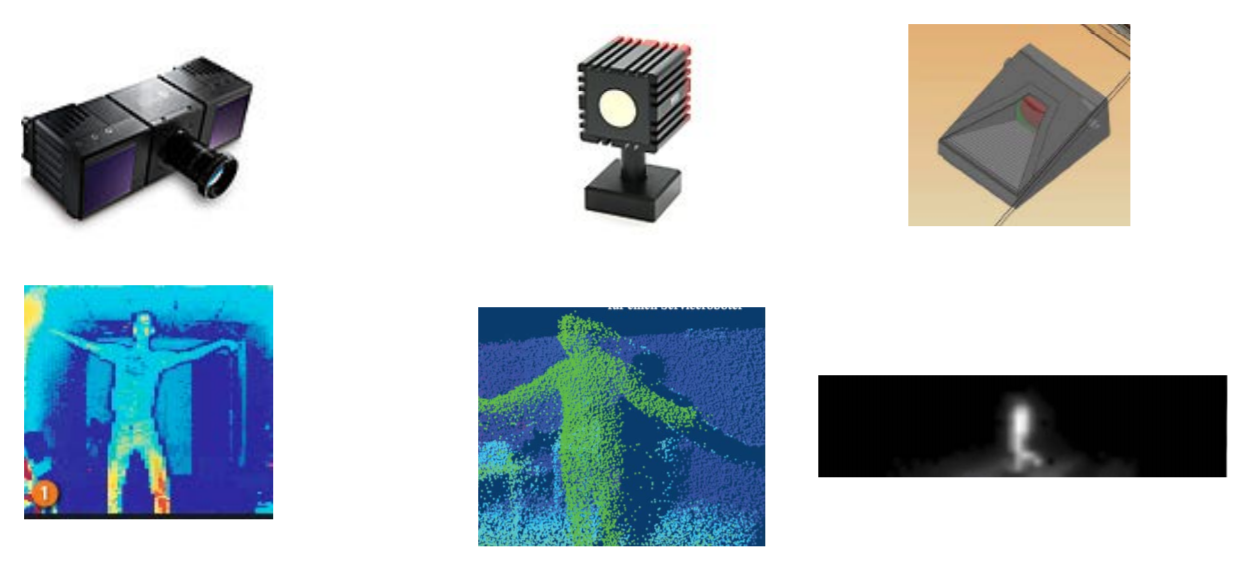
\includegraphics[width=13cm,height=13cm,keepaspectratio]{2Grundlagen/Bilder/tof_kamera.png}
    \caption{Time-of-Flight Kamera und deren Repräsentation \cite{robotik.2020m}}
    \label{pic:tofCam}
\end{figure}
\\ 
Auf der linken Seite ist eine PMD-Kamera zu sehen, gefolgt von einer SwissRanger-Kamera und auf der rechten Seite eine IFM-Kamera.
\subsection{Verfahren zur Lösung des SLAM Problems}
Das Lösen des \acs{SLAM}-Problems wird in der Praxis mit den angestellten Verfahren, die sich bei der Anwendung duchsetzten, durchgeführt. In 
folgenden Abschnitten werden zwei dieser Verfahren erläutert, sodass ein Grundverständnis vorhanden ist. Zuerst wird auf das Graph-basierte 
\acs{SLAM}, dem Lösen des Problems unter Anwendung der kleinsten-Quadrate Methode, eingegangen, darauffolgend die Lösung durch einen rekursiven 
Ansatz, dem erweiterten Kalman Filter (\acs{EKF}).

\section{Quaternionen}
\label{chap:Quaternionen}
%%%%%%%%%%%%%%%%%%%%%%%%%%%%%%%%%%%%%%%%%%%%
% -----------> tbd... !! <-----------------




%%%%%%%%%%%%%%%%%%%%%%%%%%%%%%%%

\subsection{Transformation}
\subsection{Rotation}


\section{SLAM - Simultanious Localization And Mapping}
\label{chap:SLAM}
Als Simultaneous Localization and Mapping, auch \acs{SLAM}-Problem genannt, bezeichnet man die Aufgabe, die Trajektorie\footnote{Lösungskurve oder Bewegungspfad eines Objekts} 
samt Orientierungsinformation einer sich bewegenden Plattform, z.B. ein Smartphone, Tablet oder jegliche Art von Roboter, aus 
Beobachtungen zu schätzen und gleichzeitig aus den gewonnenen Informationen eine Karte der Umgebung zu erstellen.
Diese Aufgabe ist für den weiteren Prozess bedeutend. Zum einen sollen die generierten Karten sehr präzise sein, um einen hohen 
Wert für den Nutzer oder für spezielle auf der Karte aufbauende Anwendungen darzustellen. Zum anderen benötigen autonome Roboter, 
beispielsweise Saug- oder Mähroboter, ein solch erzeugtes geometrisches Modell der Umgebung, um zielgerichtet selbstständig navigieren zu 
können. %\cite{slamdefi.2016a} 
\begin{quote}
    Das Simultaneous Localization and Mapping oder kurz SLAM Problem behandelt das gleichzeitige Schätzen der Position und Ausrichtung einer 
    mobilen Plattform im Raum anhand der sich an Bord befindlichen Sensoren sowie den Aufbau eines Modells der Umgebung. Dieses Problem ist 
    von großer praktischer Relevanz und ist Kernbestandteil der meisten mobilen Sensorsysteme. \cite{slamdefi.2016a}
\end{quote}
1986 wurden auf der \textit{IEEE Robotics and Automation Conference} erste mathematische Definitionen vorgenommen, die mittels statischer 
Theorien ermittelt und mit ersten Studien belegt wurden. Einige Jahre später, im Jahr 1995, wurde das \acs{SLAM} Problem erstmals auf dem 
internationalen Symposium für Robotikforschung (\textit{ISRR'95}) vorgestellt. Die Forschungen hielten an, bis auf der \textit{ISRR'99} 
die erste \acs{SLAM} Sitzung stattfand. 

\subsection{Definition des Problems}
Angenommen ein Roboter startet in einer Position, auch Pose genannt, und einer Konfiguration \textit{p0} und bewegt sich durch eine ihm 
unbekannte Umgebung, stellen die nicht vorhandenen Kenntnisse seiner Position und der damit verbundenen Orientierung das Hauptproblem dar. 
Die Einstellung beinhaltet Position und Ausrichtung des Roboters. Je nach Bewegung in Raum oder Ebene ist die Pose meist als 3- oder 
6-dimensionaler Vektor abgebildet. Die Bewegung des 
Roboters wird durch bekannte Kontrollkommandos \textit{u} angewiesen, allerdings mit einer gewissen Unsicherheit versehen. Dabei wird 
zwischen den Zeitpunkten \textit{t-1} und \textit{t} die Bewegung des Roboters mit \textit{ut} beschrieben und somit auch die 
unterschiedlichen Posen \textit{pt-1} nach \textit{pt}. Die Umgebung wird parallel dazu über diverse Sensoren, z.B. interne Sensoren, bspw. 
Geschwindigkeits- oder Positionssensoren, und externer Sensoren, unter anderem Abstands- oder taktile Sensoren. Neben der Protokollierung der 
Position, bei der es zu Störungen oder Berechnungsfehlern kommen kann, gibt es Beobachtungen durch Sensoren die verrauscht, bzw. fehlerhaft 
sind und durch \textit{zt} angegeben werden.
\\ 
\linebreak
Mit diesen vorhandenen Werten ist die Schätzung der Trajektorie \textit{p0:T=[p0,p1,...,pT]T} des Roboters von Beginn der 
Fortbewegung bis zum Zeitpunkt \textit{T} das Ziel. Gleichzeitig zur Berechnung der Trajektorie wird eine Karte \textit{m} des Umfelds geschätzt, 
deren Darstellung den Anforderungen entsprechend angepasst werden kann. Mit den Anforderungen sind verschiedene Repräsentationen der Karten 
gemeint, darunter beispielsweise eine Veranschaulichung von Punktansammlungen an Gegenständen, gerenderte Oberflächenmodelle oder 
2D-Rasterkarten und verstärkt visualisierte 3D-Voxelkarten\footnote{(Zusammensetzung aus dem englischen volume \textit{vox} und elements 
\textit{el}), bez. einen Gitterpunkt in einem dreidimensionalen Gitter.}. Basierend auf den Sensormessintervallen \textit{z1:T} und den dabei
stattfindenden Kontrollkommandos \textit{u1:T} wird die Karte des Umfeldes und alle Positionen bestimmt. Die Wahrscheinlichkeitsverteilung 
\textit{p(p0:T,m|z1:T,u1:T)} wird durch die geschätzten Werte \textit{p0:T} und \textit{m} berechnet. 
\\ 
\linebreak
Die Berechnung der Wahrscheinlichkeitsverteilung ist auch unter dem Namen \textit{Offline-\acs{SLAM}} bekannt. In der Praxis ist allerdings 
die Schätzung der Position \textit{xt} und der Karte der Umgebung durch \textit{p(pt,m|z1:t,u1:t)} interessanter, da Roboter Entscheidungen 
basierend auf aktuellen Informationen, z.B. der Posenschätzung und dem Umgebungsmodell, treffen sollen. Die Variante der Echtzeitschätzung 
ist auch als \textit{Online-SLAM} bekannt. \cite{slamdefi.2016a}

\subsection{Localization}
Damit das Endgerät, Smartphone oder der Roboter seine Position in Erfahrung bringen und schätzen kann, werden Informationen und Möglichkeiten 
benötigt, die Bewegung in irgendeiner Form zu messen. Da das Nutzergerät eine eigene virtuelle Karte, unabhängig von der \acs{GPS}-basierten 
Position, generiert, ist das \textit{Tracking} über die Weltkoordinaten nicht Bestandteil des eigentlichen Verfahrens. Für die Erfassung der 
internen Systemzustände gibt es sogenannte interne Sensoren die in dem Roboter zur Verfügung stehen. Bestandteile dieser internen 
Sensorik sind unter anderem Positions-, Geschwindigkeits-, Beschleunigungssensoren und das \acl{INS}. Für die Positions- und 
Geschwindigkeitserkennung gibt es z.B. einen optischen Codierer, welcher durch Lichtimpulse die Geschwindigkeit als auch die zurückgelegte 
Strecke schätzen kann. Das \acs{INS} besteht aus Lagesensoren und einem Kreiselkompass (Gyroskop). Diese sind essentiell für die Bestimmung 
der Orientierung und Neigung des Geräts. Ausgehend von der Erdkugel beziehen sich diese Sensoren auf das gegebene inertiale Koordinatensystem.
Mittels \textit{Odometrie} können die von den Sensoren bereitgestellten Informationen über Position und Orientierung berechnet werden. Radgetriebene 
Systeme führen die Berechnung durch, da diese basierend auf dem Durchmesser des Rades ermittelt wird. In Kombination mit \textit{Koppelnavigation}\footnote{Engl. dead reckoning, ist die laufende Positionsbestimmung eines bewegten Objekts infolge der Bewegungsrichtung und Geschwindigkeit \cite{koppelnavigation.2019j}}
gilt dieses Verfahren für Roboter, bzw. Fahrzeuge auf Land, als Grundlage der Navigation. Durch die theoretische Berechnung werden 
Fehlerbetrachtungen, z.B. Verschleiß, Schlupf oder Unrundheit von Rädern, vernachlässigt und ist somit nicht als alleiniges Verfahren einzusetzen. 
\begin{align}
    \Delta U = \frac{\pi D}{\textit{n}C}N
\end{align}
Mit \textit{D} als Raddurchmesser, \textit{n} als Getriebeübersetzung, \textit{C} als Enkoderauflösung und \textit{N} als Anzahl der 
Enkoderimpulse wird die Positions- und Orientierung berechnet. 
\\ 
Smartphones berechnen die Fortbewegung über gegebene Sensoren, darunter Beschleunigungs- und Neigungssensoren und Gyroskop. Dieses Zusammenspiel an 
Sensoren ermöglicht die Wahrnehmung der Positionsveränderung und kann somit diese bestimmen.
\subsection{Mapping}
Um neben der Berechnung der Position durch die interne Sensorik die Umgebung registrieren und schätzen zu können, gibt es externe Sensoren, 
die sich mit der Erfassung der Umwelt beschäftigen. Auch hier gibt es viele Arten von Sensoren, mit denen es ermöglicht wird, die Umgebung 
wahrzunehmen. Darunter sind taktile Sensoren, Näherungs-, Abstands-, Positionssensoren und visuelle Sensoren. Hinsichtlich Abstandssensoren, die 
Messungen zwischen Gegenstand und Sensor durchführen, gibt es im Allgemeinen erhebliche Vorteile gegenüber den Näherungssensoren. Unter Anderem 
besitzen sie zum Beispiel eine größere Reichweite und ein größeres Blickfeld als Näherungssensoren. Somit können sie die Entfernung zu Gegenstände 
genauer ermitteln und geometrische Umweltinformationen besser erfassen. Für die Messung des Abstandes eignet sich die \ac{TOF}-Kamera, die 
mit dem Laufzeitverfahren Distanzen messen und berechnen kann. \cite{robotik2.2020m}
\\ 
Das Laufzeitverfahren funktioniert wie folgt:
\begin{align}
    \textit{d} = \frac{1}{2}\textit{ct}
\end{align}
Abstand zwischen der Zielfläche und dem Sensor \textit{d} ist das Produkt aus der Signalgeschwindigkeit \textit{c} und der messbaren Laufzeit 
\textit{t}. Beispiele für solche \acs{TOF}-Kameras und deren Repräsentation sind folgender Abbildung (\ref{pic:tofCam}) zu entnehmen.
\begin{figure}[hbt!]
    \centering
    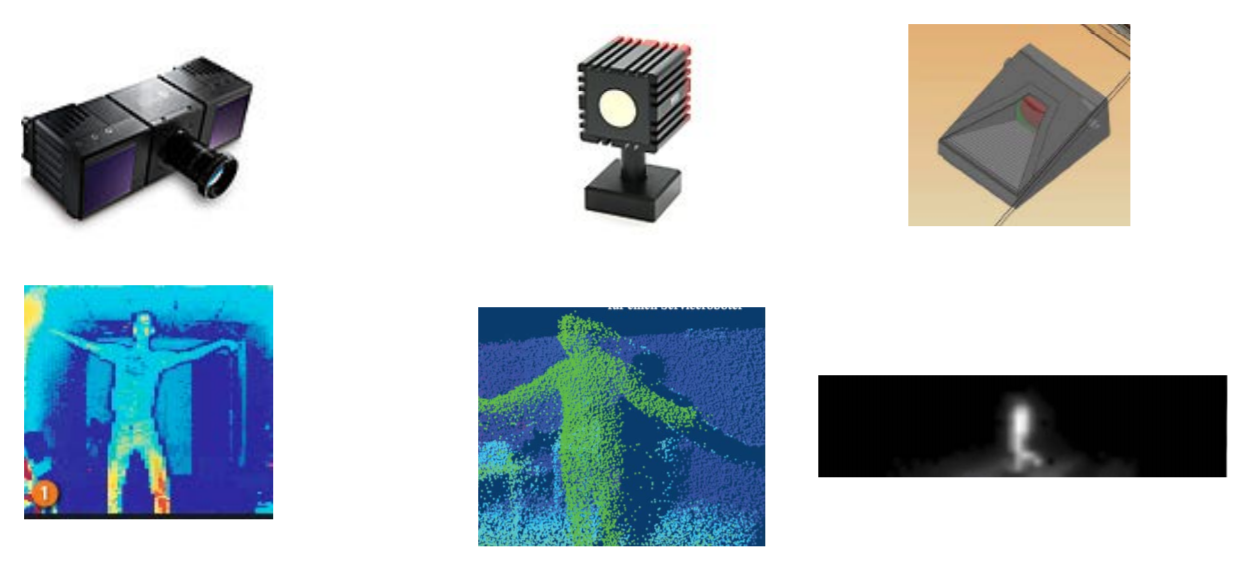
\includegraphics[width=13cm,height=13cm,keepaspectratio]{2Grundlagen/Bilder/tof_kamera.png}
    \caption{Time-of-Flight Kamera und deren Repräsentation \cite{robotik.2020m}}
    \label{pic:tofCam}
\end{figure}
\\ 
Auf der linken Seite ist eine PMD-Kamera\footnote{Photonic Mixing Device, optischer Sensor der auf dem Lichtlaufzeitverfahren beruht. Basiert auf dem TOF-Kameraprinzip} 
zu sehen, gefolgt von einer SwissRanger-Kamera und auf der rechten Seite eine IFM-Kamera\footnote{Eine erweiterte Art der 3D-Kamera}.

\subsection{Verfahren zur Lösung des SLAM Problems}
Das Lösen des \acs{SLAM} Problems wird in der Praxis mit den folgenden Verfahren, die sich bei der Anwendung bewährt haben, durchgeführt. In den 
folgenden Abschnitten werden zwei dieser Verfahren erläutert, sodass ein Grundverständnis der Funktionsweisen der Verfahren entsteht. 
Als Erstes erfolgt eine nähere Erläuterung des graph-basierten \acs{SLAM} Verfahren, gefolgt von der Lösung des Problems mit einem rekursiven 
Ansatz, dem erweiterten Kalman Filter (\acs{EKF}).

\subsection*{Graph-basiertes SLAM Verfahren}
Grundlegend wird bei dem Algorithmus des graph-basierten Verfahrens, während der Bewegungsaufzeichnung des Roboters, ein Graph modelliert, 
dessen Positionen zu verschiedenen Zeitpunkten durch Knoten dargestellt werden. Alle nebeneinander liegenden Positionen, bzw. Punkte, die 
lediglich minimale Unterschiede in der Umgebung aufweisen, werden zu einem Punkt gebündelt. Diese korrespondierenden Positionen, bzw. 
Knoten im Graphen werden über eine Kante verknüpft. Gebunden an die Bewegung des Roboters werden die Kanten modelliert. Der folgende Graph 
(\ref{pic:GraphSLAM}) veranschaulicht ein solches Modell.
\begin{figure}[hbt!]
    \centering
    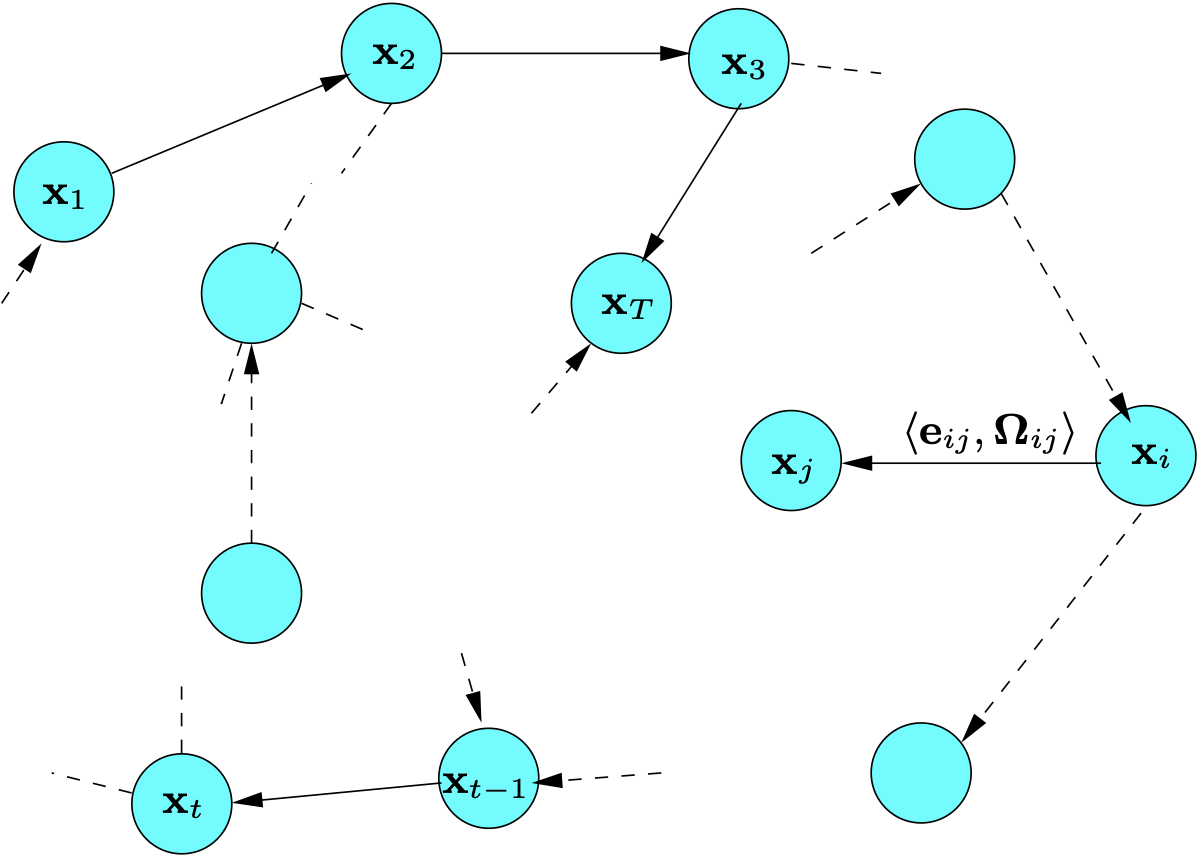
\includegraphics[width=10cm,height=10cm,keepaspectratio]{2Grundlagen/Bilder/graph_SLAM.png}
    \caption{Graphische Darstellung des SLAM Verfahrens \cite{graphSLAM.2010}}
    \label{pic:GraphSLAM}
\end{figure}
\\ 
Der Abbildung ist zu entnehmen, dass der Graph auch Kanten darstellt, die nicht den folgernden Knoten ansprechen, sondern eine 
Position vertreten, die in ihrer Beobachtung auf korrespondierende Knoten zurückgeht. Durch wiederholte Scans können genauere Merkmale und 
Bedingungen festgelegt werden, um die daraus resultierenden Positionen besser differenzieren zu können. Bei Verwendung von Kameras können 
genauer identifizierten Merkmale die geschätzten relativen Orientierungen sein, die durch eine zusätzliche Funktion berechnet werden 
können. Bei der Nutzung eines Lasersensors wird meist der \ac{ICP} Algorithmus angewendet, um die Veränderungen zwischen den Aufnahmepositionen 
wahrzunehmen. \acs{ICP} ist ein iteratives, ständig wiederholendes Verfahren, das die korrespondierenden Punkte schätzt und solange transformiert, bis diese unter 
einem gewissen Schwellwert liegen. Korrespondierende Punkte sind die, die den kleinsten Abstand zueinander haben (Closest Point). \cite{robotik2.2020m}
\\ 
Der inkrementelle Ansatz des graph-basierten \acs{SLAM} Verfahrens ist ursprünglich ein \textit{offline-Verfahren}, welches über die Jahre 
schrittweise zu einem \textit{online-Verfahren} führte. Durch diese ständige Beobachtung und Neuberechnung der aktuellen Position zu jedem 
Zeitpunkt wurde die Bedeutung der inkrementellen Verfahren gesteigert. %Dieser Ansatz ist besonders für monokulare Kameras ratsam und sinnvoll.

\subsection*{Rekursives Schätzproblem}
Der erweiterte Kalman-Filter (\acs{EKF}) ist eine wahrscheinlichkeitsbasierte rekursive Schätzung der Position des Objekts und der Position der 
Landmarken unter Nutzung linearer Bewegungsmuster basierend auf dem Bayes-Filter. Der Bayes-Filter-Algorithmus ist das generelle Verfahren der 
rekursiven Zustandsschätzung und wird über den Satz von Bayes\footnote{Mathematischer Satz der Wahrscheinlichkeitstheorie. Daruch wird die Berechnung einer bedingten Wahrscheinlichkeit beschrieben} 
hergeleitet. 
\\
Unter der Voraussetzung einer Normalverteilung und eines linearen Bewegungsmodells, worauf der Kalman-Filter setzt, kann diese durch das 
\acs{SLAM} Problem nicht erfüllt werden. An dieser Stelle wird der erweiterte Kalman-Filter eingesetzt, da dieser nicht-lineare 
Bewegungsmodelle, bzw. Funktionen mittels Taylorreihe approximiert. Somit kann eine Messung in etwas vorhergesagt werden. Diese Schätzung 
dient somit als Grundlage zur eigentlichen Messung. Nach der Berechnung wird der Zustand aktualisiert und ausgegeben. Mit diesem Ergebnis 
werden die darauffolgenden Punkte rekursiv berechnet, bis die Scan-Phase zu Ende ist.

\section{Quaternionen}
\label{chap:Quaternionen} %\cite{quaternionHamilton.2006} 
Quaternionen, lat. \textit{„Menge der Vier“}, wurden erstmals 1843 von Sir William Rowan Hamilton beschrieben. Sie bezeichnen einen 
Zahlenbereich, der die reellen Zahlen erweitert. Die mathematische Formel wird häufig zur Darstellung einer Drehung im dreidimensionalen Raum 
verwendet. Die Theorie der Quaternionen basiert auf der mathematischen Grundlage der komplexen Zahlen, die 1833 von Hamilton als Bildung 
einer Algebra galten und werden daher als hyperkomplexe Zahlen aufgefasst.
\\ 
\linebreak
Mit \textit{a,b,c,d $\in q$} werden Quaternionen wie folgt beschrieben:
\begin{align}
    \textit{q} = \textit{a} + \textit{b} \cdot \textit{i} + \textit{c} \cdot \textit{j} + \textit{d} \cdot \textit{k}
\end{align}
In oben genannter Formel ist die Variable \textit{a} der Realteil und (\textit{b,c,d})$^T$ der Imaginärteil \textit{u} der Gleichung. 
Auch geschrieben als \textit{q = (a, u)$^T$}, um die Teile differenzieren zu können. 
\\ 
Mit der sogenannten \textit{Brougham Bridge}-Formel ist es möglich Vektoren zu dividieren. 
\begin{subequations}
    \label{Quaternionen-Gleichung}
    \begin{align}
        \textit{i$^2$} = \textit{j$^2$} = \textit{k$^2$} = \textit{ijk} = \textit{-1} 
        \label{erstes Gleichungsgesetz} \\
        \textit{ij} = \textit{-ji} = \textit{k} 
        \label{zweites Gleichungsgesetz} \\
        \textit{jk} = \textit{-kj} = \textit{i} 
        \label{drittes Gleichungsgesetz} \\ 
        \textit{i$^2$} = \textit{j$^2$} = \textit{j}
    \end{align}
\end{subequations}
\subsection{Rotation}
%\subsection{Transformation}
Quaternionen dienen als Möglichkeit, Drehungen, bzw. Rotationen darzustellen, unter anderem wegen der reduzierten Anzahl an 
benötigten Parametern im Vergleich zur Berechnung von Rotationsmatrizen und deren Translation. Die Quaternionen bieten eine deutlich kompaktere 
Darstellung der Rechenwege. Somit können Rotationen intuitiver veranschaulicht werden, d.h. es sind direkte Angaben von Drehwinkel und 
-achse möglich. Die kompaktere Darbietung beinhaltet lediglich vier Werte im Vergleich zu den neun Werten der Berechnung der Rotationsmatrix
und die Rotation kann um eine bestimmte Achse ermittelt werden. Zudem ist eine sehr hohe numerische Stabilität gewährleistet. 
\\ 
Der Drehwinkel wird wie folgt berechnet:
\begin{align}
    %\textit{a} = $\cos z$ \to \textit{z} = \frac{t}{2} \to t = $\theta$  %\textit{z} = \textit{\frac{$\theta$}{2}} 
    %\\
    \textit{$\theta$} = \textit{2} \cdot \textit{$\arccos a$}
\end{align}
Der Realteil \textit{a} des Quaternions wird mittels Arkuskosinus berechnet, so erhält man die Drehung des Objekts. Die Drehachse lässt sich 
bestimmen, indem alle Werte des Imaginärteils (\textit{b,c,d})$^T$ mit \textit{u} addiert werden. Die Variable \textit{u} setzt sich wie 
folgt zusammen: 
\begin{align}
    \textit{u} = \textit{$\sin w$}, \to \textit{w} = \frac{t}{2}, \to \textit{t = $\theta$}
\end{align}
Mit diesen zwei Berechnungen werden Drehwinkel und Drehachse bestimmt und können für weitere Berechnungen verwendet werden.

\section{Technologien}
\label{chap:Technologien}                       %Programmier-Technologien
Dieser Abschnitt befasst sich mit den wichtigsten Technologien, die in diesem Projekt eingesetzt werden. 
%Ein kurzer Überblick 
%über die Historie der Technologien, worum es dabei geht und welche Aufgaben sie umfassen. 
\\ 
Der Augenmerk liegt auf dem Framework \textit{Google ARCore}, da dieses Hauptbestandteil des Projekts ist. 
\subsection{Google ARCore}
\label{sec:arcore}
ARCore ist die von Google veröffentlichte Plattform zum Erstellen von \acl{AR} Erlebnissen, primär entwickelt für Android Phones. 
Das \ac{SDK} ist in den Programmiersprachen Java und Kotlin geschrieben. Mit bestimmten \acs{API}s ermöglicht \textit{ARCore} die Erfassung 
der Umgebung durch ein Tablet oder Smartphone, um so die Welt zu verstehen. Mitte des Jahres 2017 
wurde die \textit{Google ARCore API} zum ersten Mal den Entwicklern und der \acs{AR}-Community präsentiert. Im ersten Quartal 2018 wurde 
diese dann veröffentlicht und löste das Vorreiterprojekt \textit{„Project Tango“} ab. 
\\ 
\linebreak 
\textit{Project Tango} war ebenso eine Google-Plattform, mit dem Smartphones und Tablets ein \textit{„Raumgefühl“} erhalten. \cite{projecttango.2016j} 
Die Plattform kombinierte die Eingabe verschiedener Sensoren, z.B. radarähnliche Infrarotstrahler, einer Infrarotkamera und hochpräzisen 
Beschleunigungsmessern, Barometern und Gyroskopen, um schnell nutzbare Informationen der Umgebung zu generieren. Mit der Überarbeitung des 
Konzepts wurde das neue unabhängige Projekt \textit{ARCore} geschaffen und somit die Anzahl der Hardwarekomponenten reduziert, bspw. wird 
keine spezielle Infrarotkamera mehr benötigt. Die ARCore \acs{API} verwendet bei Anwendungen ausschließlich das Kamerabild des Smartphones und 
dessen Sensoren. 
\\ 
\linebreak 
Zum Integrieren von virtuellen Objekten in die reale Welt verwendet ARCore drei Schlüsselfunktionen unter Benutzung von Java und OpenGL, Unity 
und Unreal:
\begin{itemize}
    \item Motion tracking, dt. Bewegungsverfolgung, ermöglicht das Verstehen und Verfolgen der Position des Geräts relativ zur Realität.
    \item Environmental understanding, dt. Verständnis der Umgebung, erkennt die Position und Größe aller Arten von Oberflächen: horizontale, 
    vertikale und abgewinkelte Oberflächen, wie Wände, Böden, Tische oder Stühle.
    \item Light estimation, dt. Lichtschätzung, schätzt die durch das Smartphone gegebenen Lichtverhältnisse der Umgebung. \cite{arcorefundamentals.2018m}
\end{itemize}
\begin{itemize}
    \item Motion tracking, dt. Bewegungsverfolgung, ermöglicht das Verstehen und Verfolgen der Position des Geräts relativ zur Realität.
    \item Environmental understanding, dt. Verständnis der Umgebung, erkennt die Position und Größe aller Arten von Oberflächen: horizontale, 
    vertikale und abgewinkelte Oberflächen, wie Wände, Böden, Tische oder Stühle.
    \item Light estimation, dt. Lichtschätzung, schätzt die durch das Smartphone gegebenen Lichtverhältnisse der Umgebung. \cite{arcorefundamentals.2018m}
\end{itemize}
\subsubsection*{Motion tracking}
Für die Funktion der Bewegungsverfolgung verwendet ARCore das Verfahren von \acl{SLAM} (\acs{SLAM}) \ref{chap:SLAM}, um so zu verstehen wo 
sich das Smartphone in Relation zur realen Welt befindet. Zusätzlich erkennt ARCore visuell unterschiedliche Merkmale im aktuell aufgenommenen 
Kamerabild, sogenannte Merkmalspunkte \textit{„feature points“}. Anhand dieser Punkte wird die Änderung des Standortes berechnet. Durch Trägheitsmessungen 
der \ac{IMU}, dt. Inertiale Messeinheit des Geräts, kombiniert mit den visuellen Informationen des Kamerabildes wird die Position und 
Ausrichtung der Kamera in Relation zur Realität abgeschätzt. \cite{arcoreofficial.2020j}
%\begin{figure}[hbt!]
%    \centering
%    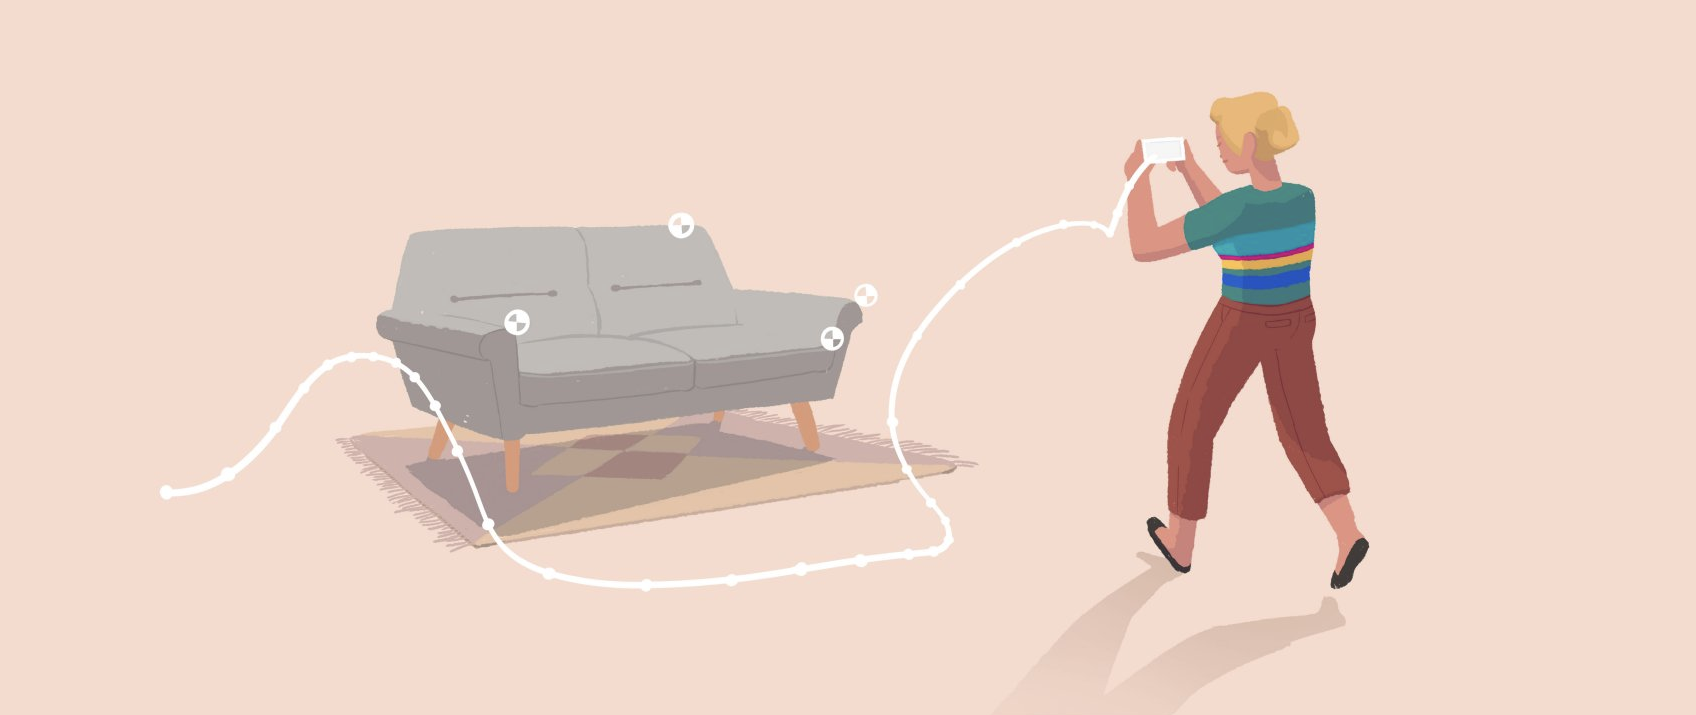
\includegraphics[width=15cm,height=5cm,keepaspectratio]{2Grundlagen/Bilder/motionTracking.png}
%    \caption{Skizze zur Bewegungsverfolgung des Smartphones \cite{arcoreofficial.2020j}}
%    \label{pic:motiontracking}
%\end{figure}
\\
\linebreak 
Die \acl{IMU} in Smart-Devices besitzt drei Beschleunigungssensoren, z.B. piezoelektrische Beschleunigungssensoren oder \ac{MEMS}, für die 
drei Raumachsen:
\begin{itemize}
    \item Die Abszissenachse (X-Achse), die horizontale (waagerechte) Koordinatenachse, \cite{bianco.2016}
    \item Die Ordinatenachse (Y-Achse), die darauf vertikale (senkrechte) Koordinatenachse \cite{bianco.2016} und
    \item Die Applikatenachse (Z-Achse), die auf beiden anderen Achsen senkrechte Achse \cite{koordinatennorm.1973m}
\end{itemize}
Ebenso besitzt die \acs{IMU} Drehratensensoren, z.B. ein Gyroskop zur Messung der Rotationsgeschwindigkeit, welche die Drehraten um 
diese Raumachsen messen. \cite{imubild.2020j} Durch die kontinuierliche Auslesung der Sensordaten, wird die Position des Geräts berechnet und in Form von 
drei Koordinaten ausgegeben. Ausgehend von dem Referenzkoordinatensystem wird die Position neu bestimmt. Die Abbildung \ref{pic:Positionsberechnung} 
veranschaulicht solch ein Beispiel.
\begin{figure}[hbt!]
    \centering
    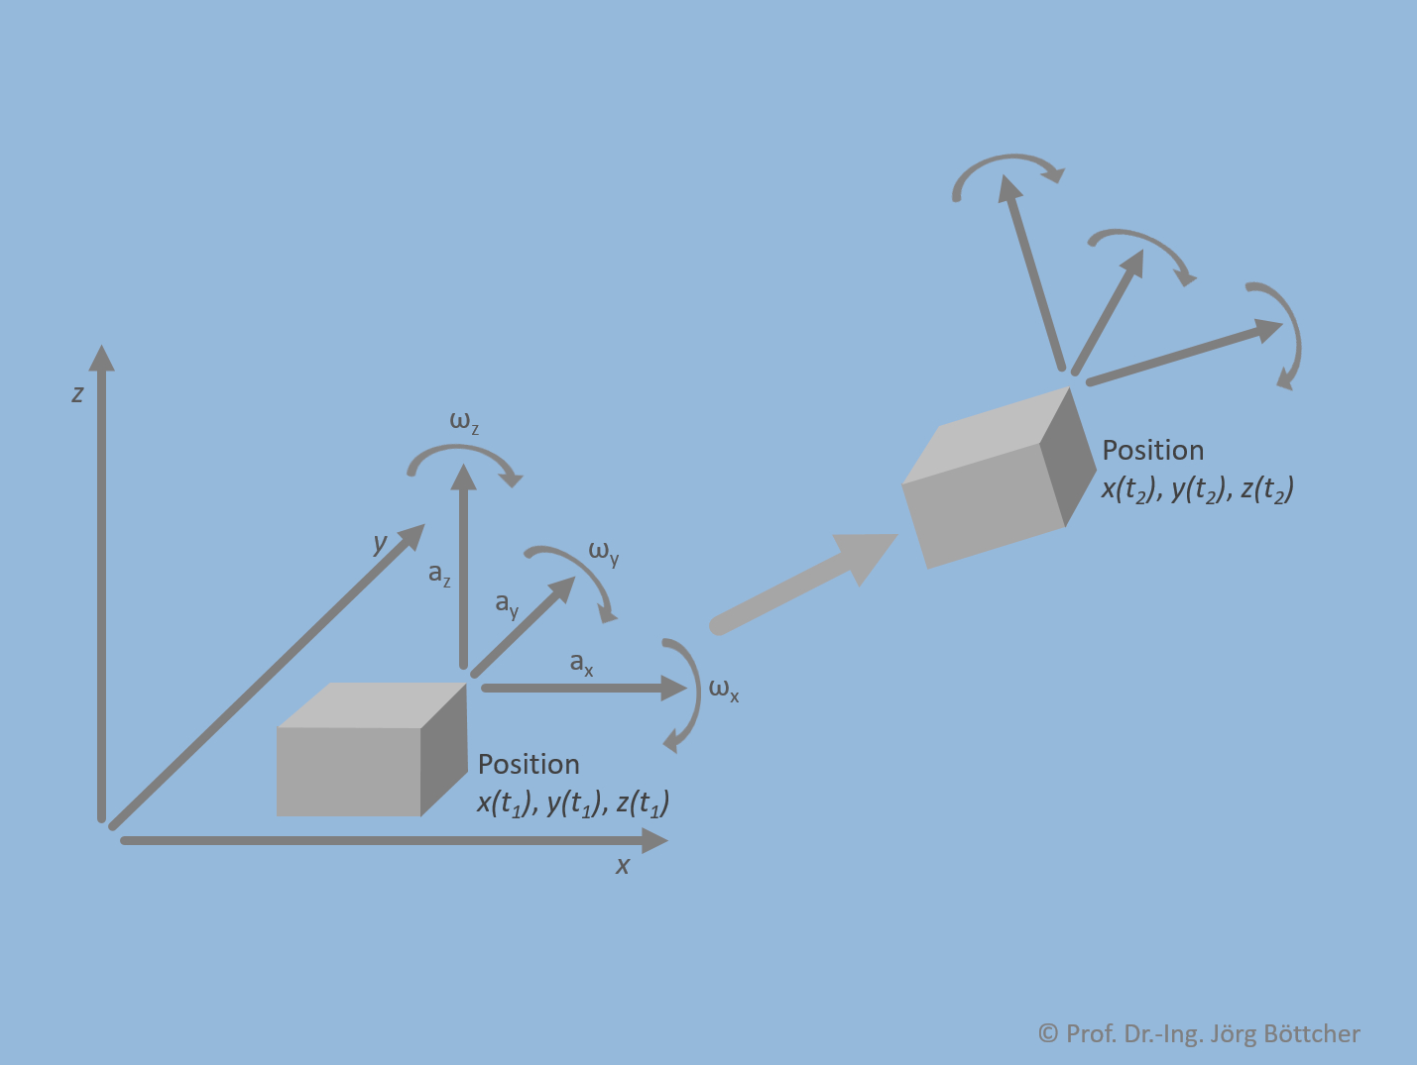
\includegraphics[width=9cm,height=9cm,keepaspectratio]{2Grundlagen/Bilder/imu-Bsp.png}
    \caption{Grundprinzip einer IMU \cite{imubild.2020j}}
    \label{pic:Positionsberechnung}
\end{figure}
\pagebreak
\subsubsection*{Environmental understanding}
Die zweite Schlüsselfunktion des Frameworks ist das Verständnis der Umgebung. Dieses wird erlangt, indem \textit{„feature points“}, Ebenen und 
Flächen beim Scannen des Umfelds erkannt werden. Beim Entstehen mehrerer solcher \textit{feature points} erstellt ARCore ein Cluster aller 
naheliegenden Punkte. Dieses erzeugte Cluster repräsentiert eine horizontale oder vertikale Fläche. Mit diesen gewonnenen Informationen ist das 
Platzieren von virtuellen Objekten auf den erfassten Flächen möglich. \cite{arcoreofficial.2020j}
%\begin{figure}[hbt!]
%    \centering
%    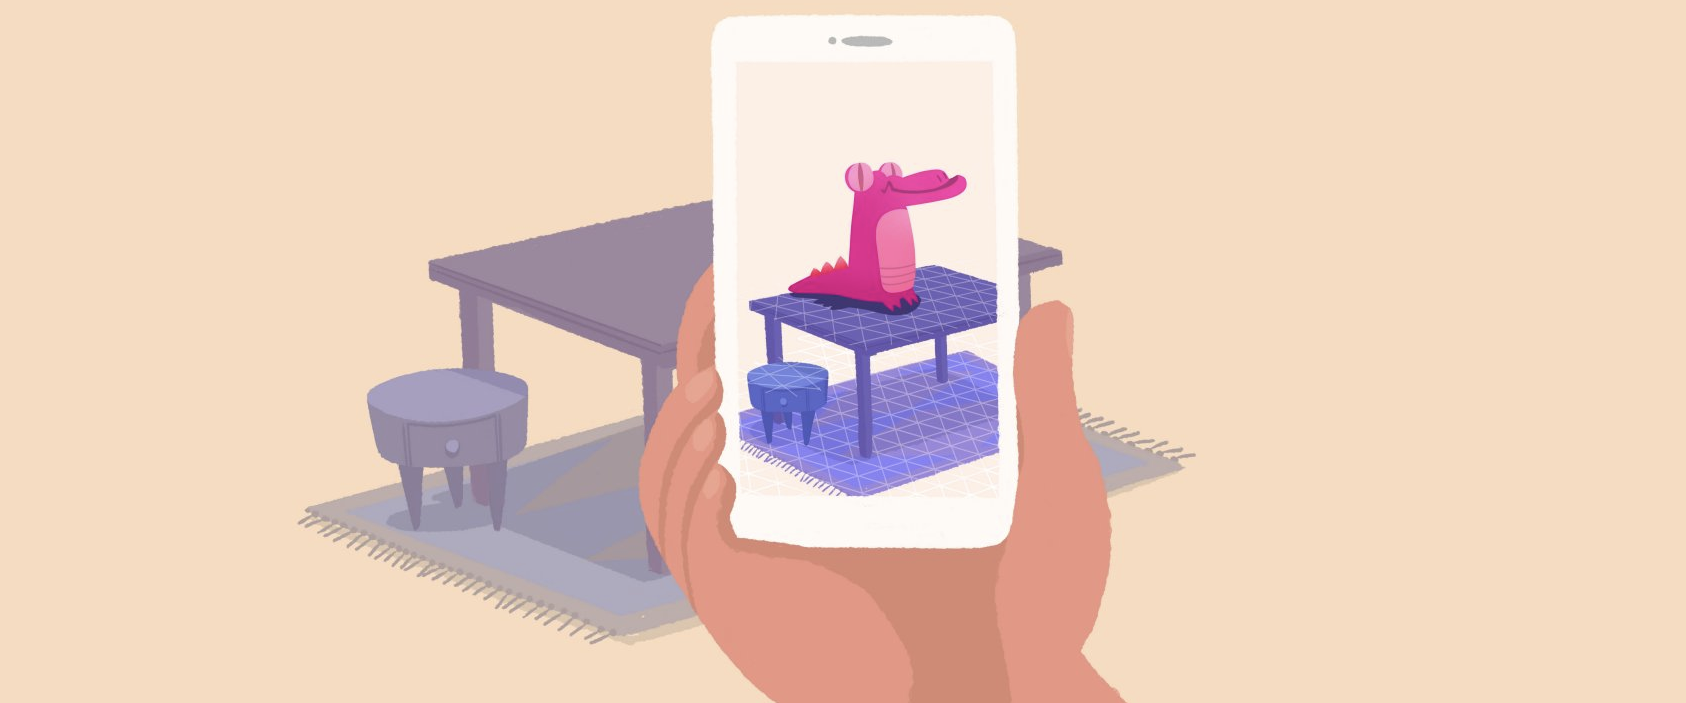
\includegraphics[width=15cm,height=5cm,keepaspectratio]{2Grundlagen/Bilder/environmentalUnderst.png}
%    \caption{Skizze zum Umgebungsverständnis des Smartphones \cite{arcoreofficial.2020j}}
%    \label{pic:environmentalunderst}
%end{figure}
\subsubsection*{Light estimation}
Mit der Funktion der Lichtschätzung kann ARCore Lichtverhältnisse und Informationen über die Beleuchtung der Umgebung erkennen. Dadurch kann das 
\acs{SDK} durchschnittliche Intensität und eine angepasste Farbkorrektur eines bestimmten Kamerabildes liefern, um so die Aufarbeitung des Bildes 
der Umgebung anzupassen. Diese Funktion verstärkt die Anpassung des virtuellen Objektes an die Realität und lässt dieses noch glaubwürdiger 
erscheinen. \cite{arcoreofficial.2020j}
%\begin{figure}[hbt!]
%    \centering
%    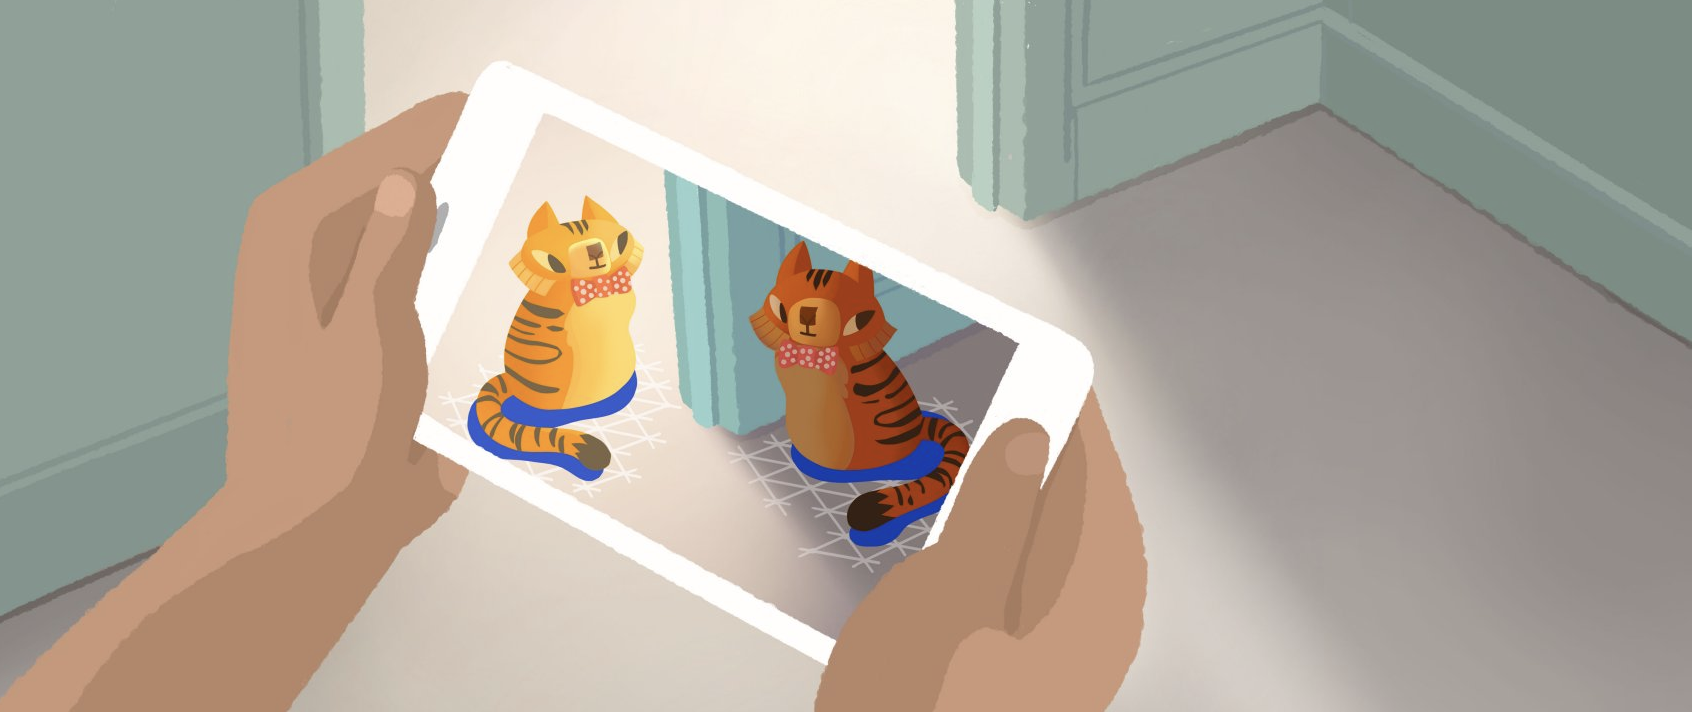
\includegraphics[width=15cm,height=5cm,keepaspectratio]{2Grundlagen/Bilder/lightEstim.png}
%    \caption{Skizze zu den Lichtverhältnissen des Smartphones \cite{arcoreofficial.2020j}}
%    \label{pic:lightestim}
%end{figure}
\subsection{Android Jetpack}
\label{sec:androidjetpack}
Android Jetpack ist eine Ansammlung an Bibliotheken, die es Entwicklern ermöglicht \textit{Best Practices} zu befolgen, 
Boilerplate\footnote{Sind Codeabschnitte, die an mehreren Stellen mit wenigen oder gar keinen Änderungen aufgeführt sein müssen. \cite{boilerplate.2019m}}-Code 
zu reduzieren.
%und Quell-/ Source-Code zu schreiben.
Die durch Android Jetpack zur Verfügung gestellten Bibliotheken fördern die konsistente Funktionsweise der 
Android-Versionen und -Geräten. Darüber hinaus wird mit Android Jetpack ein Überblick verschafft, um Best Practices und empfohlene 
Architekturen zu berücksichtigen.
\\ 
Außerdem wurde Android Jetpack für moderne Design-Praktiken entwickelt, darunter fällt \textit{„seperation of concerns“}\footnote{(SoC), Entwurfsprinzip, um verschiedene Verantwortlichkeiten auf 
verschieden Abschnitte zu trennen. \cite{soc.2019a}}, \textit{testability}, \textit{loose coupling}, \textit{Observer Pattern}\footnote{Beobachter-Muster, Verhaltensmuster der GoF-Muster}, 
\textit{Inversion of Control}\footnote{(IoC), Umsetzugsparadigma, das ein spezifisches Objekt über ein mehrfach verwendetes Objekt aufruft. \cite{ioc.2020}} und 
\textit{productivity features}, z.B. Plugin-Integrationen. Dies sind Techniken, um eine robuste und qualitativ hochwertige App zu erstellen.
\\ 
Die Bibliothekensammlung ist die Grundlage für die verwendete Architektur, Android Architecture Components in Abschnitt \ref{chap:AAC}.
%\\ 
%\linebreak
%Die Abbildung \ref{pic:androidjetpackcomp} zeigt einen Überblick über die in Jetpack enthaltenen Bibliotheken. % in Abschnitt \ref{chap:AAC}
%\begin{figure}[hbt!]
%    \centering
%    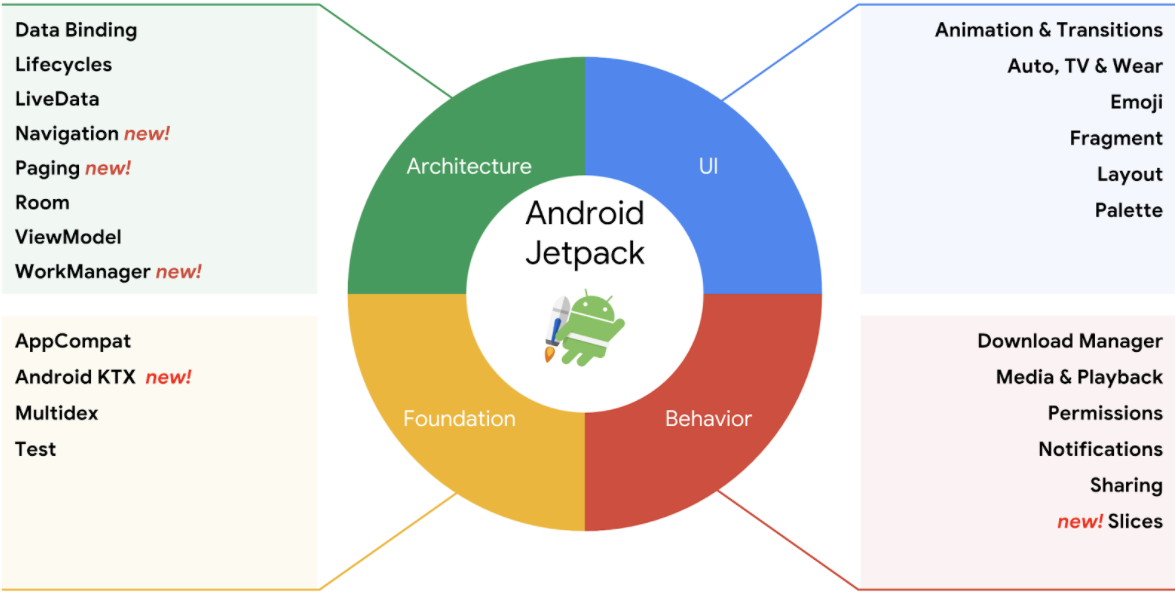
\includegraphics[width=15cm,height=10cm,keepaspectratio]{2Grundlagen/Bilder/androidjetpackcomps.png}
%    \caption{Komponenten von Android Jetpack \cite{androidjpdescr.2018m}}
%    \label{pic:androidjetpackcomp}
%\end{figure}
%\\
%Eine nähere Erläuterung aller Bibliotheken findet im Rahmen dieser Ausarbeitung nicht statt, wobei die zur Verwendung geplanten 
%„Architecture Components“ beschrieben werden. 
\\ 
\linebreak
LiveData, Room und ViewModel sind Bestandteil der \textit{Android Architecture Components}-Konstellation 
und bilden die Basis für die Architektur, welche an das \textit{MVVM-Pattern} angelehnt ist.

\subsection*{LiveData}
\label{sec:LiveData}
\textit{LiveData} gehört zu den \textit{Observer-Pattern} und ist eine Datenhalterklasse die eine Beobachtungsfunktion, bzw. -charakter besitzt. Der 
Unterschied zu einem regulären Observable ist, die lebenszyklus-unabhängige LiveData-Komponente. Dies bedeutet, der Lebenszyklus anderer 
Komponenten z.B. \textit{Activities, Fragments oder Services}, wird berücksichtigt. Mit dieser Kenntnis wird sichergestellt, dass LiveData 
nur App-Komponenten beobachtet, welche sich in einem aktiven Lebenszyklus befinden. \cite{liveData}
\\ 
\linebreak
Vorteile, die die \textit{LiveData}-Komponente mit sich bringt, sind unter anderem die Sicherstellung der Übereinstimmung der Benutzeroberfläche und 
deren Datenstatus, vorbeugend gegenüber Speicherverlust, immer auf dem aktuellsten Stand der gespeicherten Informationen und dem Wegfall 
der manuellen Lebenszykluskoordination. \cite{livedata.2020}
\subsection*{Room}
\label{sec:Room}
\textit{Room} ist eine Persistenzbibliothek und bietet ein Abstraktionsschicht über der eigentlichen \textit{\acs{SQL}ite}-Datenbank, um einen 
robusten Datenbankzugriff zu managen und das volle Potential von \acs{SQL}ite gleichzeitig zu nutzen. \cite{room.2017}
%\\ 
%\linebreak
Die robuste \acs{SQL}-Objektzuordnungsbibliothek \textit{Room} kann einen Cache mit den Daten der Applikation auf einem Gerät erstellen. Dieser 
Cache dient als Wahrheitsquelle der Applikation und ermöglicht den Benutzern eine konsistente Kopie der Informationen der App anzuzeigen 
und immer zugänglich zu machen. \textit{Room} kann in drei Kategorien, bzw. in drei Hauptkomponenten unterteilt werden:
\begin{itemize}
    \item Room database: Dient als Zugriffspunkt für die zugrundeliegende SQLite-Datenbank
    \item DAO (Data Access Object): Beinhaltet Methoden um Datenbankzugriffe zu gewährleisten.
    \item Entity: Repräsentiert ein Objekttabelle der Datenbank.
\end{itemize}
Das Diagramm \ref{pic:roomarchitecturediagramm} veranschaulicht die Interaktion, bzw. Funktionsweisen der Hauptkomponenten.
\begin{figure}[hbt!]
    \centering
    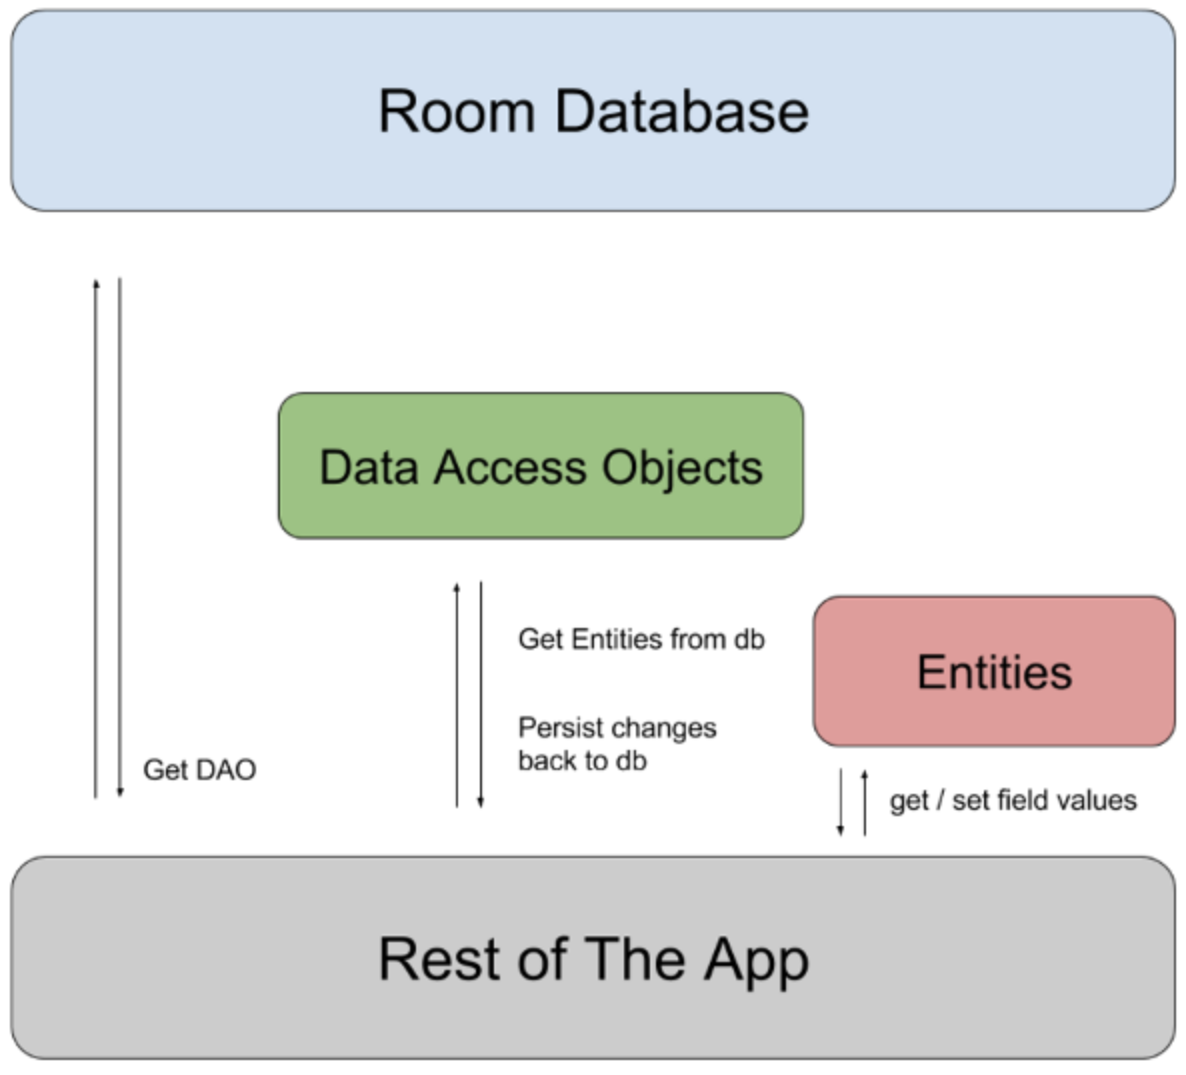
\includegraphics[width=8.5cm,height=8.5cm,keepaspectratio]{2Grundlagen/Bilder/roomArchitecture.png}
    \caption{Room Architektur Diagramm \cite{roomdiagr.2017}}
    \label{pic:roomarchitecturediagramm}
\end{figure} 
\pagebreak
\\
%\linebreak
Allgemein ermöglicht \textit{Room} einen vereinfachten Zugriff auf die Datenbank. Die Bibliothek bietet dadurch eine hohe \textit{„testability“}. 
Zur Kompilierungszeit wird eine \acs{SQL}-Abfrageüberprüfung durchgeführt. \textit{Room} interagiert einwandfrei mit anderen Android Architecture 
Components, z.B. LiveData und ViewModel.

\subsection*{ViewModel}
\label{sec:ViewModel}
Grundsätzlich dient das \textit{ViewModel} als lebenszyklusbewusste Speicherung und Verwaltung von benutzeroberflächenbezogenen Daten. 
Durch die \textit{ViewModel}-Klasse können Informationen Konfigurationsänderungen, z.B. Bildschirmdrehungen, die als Änderung zählen, 
überstehen. Eine Konfiguration kann sog. Activities verwerfen und neu laden, so können nicht persistierte Daten verloren gehen. \cite{viewModelAndroid.2020}
\\ 
\linebreak
Ein \textit{ViewModel} fungiert ebenso als Kommunikationsschnittstelle zwischen den darüber- und darunterliegenden Komponenten der 
Architektur (siehe Abschnitt \ref{chap:AAC}). Des Weiteren kann die \textit{ViewModel}-Komponente Informationen zwischen Benutzeroberflächen 
und verschiedenen Fragmenten, engl. \textit{„fragments“}\footnote{Teil einer \ac{UI} in einer Android Activity}, teilen.
\\ 
\linebreak
Die Abbildung \ref{pic:viewModeldiagramm} zeigt eine sich ändernde Activity, die zu Beginn und nach Neuerstellung oder Aktualisierung Zugriff 
auf die unveränderten Daten hat. 
\begin{figure}[hbt!]
    \centering
    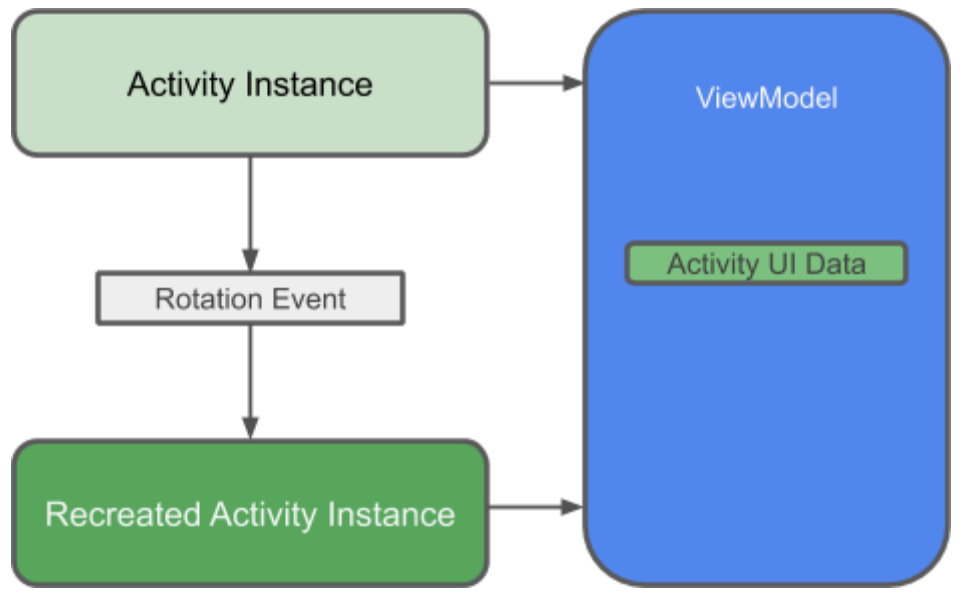
\includegraphics[width=8.5cm,height=8.5cm,keepaspectratio]{2Grundlagen/Bilder/viewModelDiagram.png}
    \caption{ViewModel Struktur Diagramm \cite{viewmodeldiagr.2020}}
    \label{pic:viewModeldiagramm}
\end{figure} 
\pagebreak
\subsection{Sceneform SDK}
Das Sceneform \acs{SDK} ist ein Open-Source Projekt der Google LLC., welches für das Rendern von 3D-Szenen und -Animationen zuständig ist. 
Basierend auf der physikalischen Echtzeit-Rendering-Engine, \textit{physically based renderer} für Android, iOS, macOS, Linux und Windows 
von Google Filament, wurde Sceneform entwickelt. \cite{sceneform.2020}
\\ 
\linebreak
Bei dem Ansatz des physikalisch basierten Renderns in der Computergrafik wird versucht, alle Modalitäten der realen Welt genauer zu modellieren. 
Mit dieser Methode werden virtuelle 3D-Objekte in der \acl{AR} noch realer dargestellt, um einen Echtheitseffekt zu erzielen und zu simulieren. 
Ein Beispiel ist das Simulieren des Lichtflusses, um einen Schatten des Objekts zu erzeugen, wodurch die Wirksamkeit immer mehr der Realität 
entspricht.
\\ 
\linebreak
Dreidimensionale Modelle werden als \textit{(.obj)}-Dateien in das Projekt importiert. Diese Dateien beinhalten aufgelistete Punkte, Vektoren 
und Linien, welche das Modell repräsentieren. Das \textit{Sceneform \acs{SDK}} verwendet die \textit{.obj}-Datei und konvertiert, bzw. 
rendert diese in eine, \textit{Sceneform binary assets (.sfb)}-Datei. Diese generierte Datei ermöglicht das Generieren eines dreidimensionalen 
Objekts, welches anschließend in \acs{AR}-Anwendungen basierend auf Google ARCore verwendet werden kann. 
Für die finale Renderung und Anzeige ist die \textit{ModelRenderable}-Klasse des \acs{SDK}s zuständig. 
%\\ 
%\linebreak
%Ein weiterer wichtiger Aspekt diese Projekts ist der Einsatz einer Datenbank, um generierte Daten speichern zu können.
\subsection{SQLite}
\acs{SQL}ite ist eine Open-Source In-Process-Bibliothek, die ein in sich geschlossenes, serverloses, transaktionsfreies \acs{SQL}-Datenbankmodul 
ohne Konfiguration implementiert. \acs{SQL}ite ist eine eingebettete \acs{SQL}-Datenbank-Engine die im Gegensatz zu anderen \acs{SQL}-Datenbanken über 
keinen separaten Serverprozess verfügt, d.h. Transaktionen, Lese- und Schreibzugriffe werden direkt auf eine normale Festplattendatei getätigt. \cite{sqlite.2018j}
\\
Darüber hinaus ist \acs{SQL}ite plattformübergreifend und kann beliebig Datenbank- und Objekttabellen, Indizes und Ansichten erstellen und verwalten.
%%%%%%%%%%%%%%%%%%%%%%%%%%%%%%%%%%%%%%%%%%%%%%%%%%%%%%%%%%%%%%%%%%%%%%%%%%%%%
%% Descr:       Vorlage für Berichte der DHBW-Karlsruhe, Ein Kapitel
%% Author:      Prof. Dr. Jürgen Vollmer, vollmer@dhbw-karlsruhe.de
%% $Id: kapitel2.tex,v 1.5 2017/10/06 14:02:51 vollmer Exp $
%%  -*- coding: utf-8 -*-
%%%%%%%%%%%%%%%%%%%%%%%%%%%%%%%%%%%%%%%%%%%%%%%%%%%%%%%%%%%%%%%%%%%%%%%%%%%%%%%

%\section{OpenGL}
%\label{chap:OpenGL}
%\subsection{Projektionen}
%\subsection{Shader}

\section{Softwarearchitektur}
\label{chap:Softwarearchitektur}
Komponenten in Form von Klassen, Objekten oder Bibliotheken und deren Verbindungen zwischen einzelnen Komponenten beschreibt die Architektur 
eines Softwaresystems. Vielmehr geht es bei der Software-Architektur darum, Anforderungen und deren Zusammenhänge untereinander von dem zu 
konstruierenden System zu beschreiben und nicht einen detaillierten Entwurf vorzulegen. Jedoch hat die Architektur einen enormen Einfluss 
auf die qualitativen und nicht-funktionalen Eigenschaften des daraus resultierenden Systems. 
\\ 
\linebreak
Die Terminologie nach dem \textit{IEEE-Standard 1471-2000} zur Software Architekturbeschreibung, deren Aufgaben und Zweck \cite{swarchitekturieee.2005} 
sind wie folgt definiert: 
\begin{quote}
    Die grundlegende Organisation eines Systems, dargestellt durch dessen Komponenten, deren Beziehungen zueinander und zur Umgebung sowie den 
    Prinzipien, die den Entwurf und die Evolution des Systems bestimmen. \cite{architektursw.2006f}
\end{quote}
Softwarearchitektur bietet viele Möglichkeiten ein System zu entwerfen und Anforderungen und Eigenschaften umzusetzen, daher gibt es auch 
hier viele Ansätze, Lösungen und Abwandlungen, um den Standards und Richtlinien gerecht zu werden. Beispiele dafür sind unter anderem die 
Modulare Software Architektur (\ref{chap:Modulare Software Architektur}) und das Architektur-Entwurfsmuster MVVM (\ref{chap:MVVM}).
\\
Das Buch \textit{Design Patterns - Elements of Reusable Object-Oriented Software} von E. Gamma, R. Helm, R. Johnson und J. Vlissides befasst 
sich mit den verschiedensten Möglichkeiten und Ausprägungen der Softwarearchitektur. 
\\ 
Im Rahmen dieser Ausarbeitung findet keine Aufzählung und Beschreibung verschiedener Arten der Architekturmuster und -stile statt, lediglich die 
für das Projekt verwendeten Muster werden in folgenden Kapiteln aufgegriffen. 
\\ 
\linebreak
Die Abbildung \ref{pic:mvcdiagram} veranschaulicht eine vereinfachte Struktur eines Architekturmusters und deren Komponenten und Zusammenhänge 
zueinander. Die Zeichnung dient zur Veranschaulichung, um darzulegen wie ein Architekturdiagramm aussehen kann, bzw. wie die allgemeine 
Struktur repräsentiert wird.
\begin{figure}[hbt!]
    \centering
    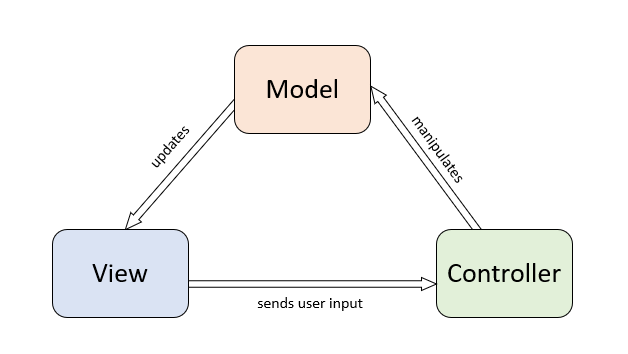
\includegraphics[width=15cm,height=7.5cm,keepaspectratio]{2GrundlagenX/Bilder/MVCArchitecture.png}
    \caption{MVC Architektur Diagramm \cite{mvcbild.2020}}
    \label{pic:mvcdiagram}
\end{figure} 
Im Falle dieser Abbildung wurde das Strukturmuster \ac{MVC} ausgewählt, welches die zu sehenden Komponenten in drei in sich 
geschlossene und unabhängige Fragmente unterteilt die miteinander interagieren. 
\\ 
\linebreak
Neben der Strukturierung von Systemen und Applikationen kann die Modellierung einer Softwarearchitektur auch dabei helfen eine Architektur genauer 
zu beschreiben und zu dokumentieren. Ebenso können Diagramme auch das Management sowie die Planung beeinflussen und verstärken. Die Modellierung 
der Softwarearchitektur stellt somit keinen Selbstzweck dar, sondern bietet einen Mehrwert indem es zur Verständigung, Dokumentation und 
Kommunikation zwischen Entwicklern und Kunden zusätzlich beiträgt. 
\\ 
Durch die Modellierung der Architektur kann frühzeitig eine sinnvolle Evaluierung und Bewertung des Entwurfs durchgeführt werden. Mit diesen 
entstehenden Bewertungen können folgende Schritte besser geplant und umgesetzt werden. 
\\ 
\linebreak
Eine weitere Variante, bzw. Ausprägung der Software-Architektur ist die Modulare Software Architektur (siehe Abschnitt \ref{chap:Modulare Software Architektur}).
\subsection{Modulare Software Architektur}
\label{chap:Modulare Software Architektur}
Der Begriff Modularität beschreibt die Art dieser Software-Architektur passend. Modularität bezeichnet die Aufteilung eines großen Ganzen in 
mehrere kleinere Teile, die als Module, Komponenten oder Bausteine beschrieben werden. Verschiedene Teile können bei geeigneter Funktion 
und Kompatibilität zusammengeführt werden oder über entsprechend definierte Schnittstellen interagieren. 

\subsection{MVVM}
\label{chap:MVVM}
\subsection{Android Architecture Components}
\label{chap:AAC}



\section{Datenmodellierung}
\label{chap:Datenmodellierung}
%%%%%%%%%%%%%%%%%%%%%%%%%%%%%%%%%%%%%%%%%%%%%%%%%%%%%%%%%%%%%%%%%%%%%%%%%%%%%
%% Descr:       Vorlage für Berichte der DHBW-Karlsruhe, Ein Kapitel
%% Author:      Prof. Dr. Jürgen Vollmer, vollmer@dhbw-karlsruhe.de
%% $Id: kapitel2.tex,v 1.5 2017/10/06 14:02:51 vollmer Exp $
%%  -*- coding: utf-8 -*-
%%%%%%%%%%%%%%%%%%%%%%%%%%%%%%%%%%%%%%%%%%%%%%%%%%%%%%%%%%%%%%%%%%%%%%%%%%%%%%%

\chapter{Konzeption}
\label{chap:Konzeption}
In diesem Kapitel wird das erarbeitete Konzept dieser Ausarbeitung dargelegt. Unter dessen die Überlegungen zu einzelnen 
Arbeitsschritten und dem grundsätzlich angedachten Aufbau des Projekts, sowie Entscheidungs- und Beweggründe wieso bestimmte 
Technologien gewählt wurden. Zu Beginn wird auf die Einsatzmöglichkeiten (\ref{chap:Arbeitsumgebung}), in der die Applikation Anwendung 
finden könnte, eingegangen. Anschließend werden die Grundgedanken zu den einzelnen Phasen, Scan-Phase (\ref{chap:Scan-Phase}) und 
Visualisierungs-Phase (\ref{chap:Visualisierungs-Phase}) des Systems erläutert, was sie beinhalten und wie sie funktionstechnisch 
angedacht sind. Mit den zugrundeliegenden Informationen wird auf das Architekturkonzept (\ref{chap:Architekturkonzept}), sowie auf das 
Softwarekonzept (\ref{chap:Architekturkonzept}) eingegangen. Des Weiteren werden die Hintergründe der Wahl des AR-Frameworks 
(\ref{chap:Auswahl des AR Frameworks}) aufgezeigt und abschließend wird noch das konzipierte und prototypische Datenmodell 
(\ref{chap:Datenmodell}) dargelegt.

\section{Arbeitsumgebung / Umfeld}
\label{chap:Arbeitsumgebung}

\section{Objekterkennung / Scan-Phase}
\label{chap:Scan-Phase}

\section{Visualisierungs-Phase}
\label{chap:Visualisierungs-Phase}

\section{Architekturkonzept}
\label{chap:Architekturkonzept}

\section{Softwarekonzept}
\label{chap:Softwarekonzept}

\section{Auswahl des AR Frameworks}
\label{chap:Auswahl des AR Frameworks}
Mittlerweile gibt es eine enorme Auswahl an \acs{AR}-Frameworks, die alle unterschiedlich unterschiedliche Präferenzen und 
Einsatzmöglichkeiten haben. Somit sind, auf den Bereich bezogen, Vor- und Nachteile im Vergleich von mehrere Frameworks nicht ausgeschlossen. 
Einige Alternativen wurden getestet und auf deren Brauchbarkeit evaluiert und analysiert. Dazu wurden Kriterien ausgearbeitet, die die 
Auswahl an Frameworks einschränken und nach Möglichkeit das passendste ergeben sollte: 
\begin{enumerate}
    \item Eine performante Darstellung von Objekten.
    \item Möglichkeiten zur Positionsbestimmung.
    \item Eine aktive Community und stetige Weiterentwicklung des Systems.
    \item Möglichkeit zur Integration weiterer Technologien.
    \item Open Source-Projekt, um Flexibilität und weitestgehende Unabhängigkeit zu gewährleisten.
\end{enumerate}
Aufgrund der großen Anzahl an \acs{AR}-Frameworks war es nicht möglich alle in betracht gezogenen Frameworks detailliert aufzuführen, 
lediglich die engere Auswahl der Tools wird aufgegriffen. 
\\ 
Nach ausführlicher Recherche wurden letzten Endes drei Frameworks in die nähere Auswahl aufgenommen, darunter \textit{vuforia}, 
\textit{ARToolkit} und \textit{Google ARCore}. Beweggründe zu dieser Entscheidung war die überwiegende 
Übereinstimmung zu zuvor aufgestellten Kriterien und Anforderungen. Alle Technologien konnten eine aktive und große Community, sowie eine 
aktive Entwicklung, bzw. Weiterentwicklung vorweisen. Zusätzlich bieten alle Frameworks viele Möglichkeiten zur Integration weiterer 
Technologien, um nach Belieben immer mehr Funktionen in das zu entwickelnde System zu übernehmen. Die Performance der Technologien konnte 
in allen Aspekten überzeugen und ist unter einfachen Bedingungen mehr als ausreichend. Ein Kritikpunkt gegen die Verwendung von vuforia war 
die fehlende Verfügbarkeit des Quellcodes, da dieser unter kostenpflichtiger Lizenz steht und nicht als Open Source-Projekt gilt. 
\subsection{Google ARCore}
\subsection{ARToolKit}

\section{Datenmodell}
\label{chap:Datenmodell}

%%%%%%%%%%%%%%%%%%%%%%%%%%%%%%%%%%%%%%%%%%%%%%%%%%%%%%%%%%%%%%%%%%%%%%%%%%%%%
%% Descr:       Vorlage für Berichte der DHBW-Karlsruhe, Ein Kapitel
%% Author:      Prof. Dr. Jürgen Vollmer, vollmer@dhbw-karlsruhe.de
%% $Id: kapitel2.tex,v 1.5 2017/10/06 14:02:51 vollmer Exp $
%%  -*- coding: utf-8 -*-
%%%%%%%%%%%%%%%%%%%%%%%%%%%%%%%%%%%%%%%%%%%%%%%%%%%%%%%%%%%%%%%%%%%%%%%%%%%%%%%

\chapter{Umsetzung}
\label{chap:Umsetzung}
Dieses Kapitel greift die in der Konzeption (\ref{chap:Konzeption}) aufgeführten Planungen und Ideen auf und legt die Implementierung, bzw. 
Umsetzung detaillierte dar. Darunter werden Lösungsansätze aufgezeigt und aufgetretene Probleme und deren Behebung dokumentiert. Allgemein die Umsetzung 
des Startmenüs und der beiden Kernfunktionen sowohl die Frontend- als auch die Backend-Aspekte werden in der Implementierung (\ref{chap:implementierung}) 
aufgezeigt. Abschließend zu dem Kapitel wird ein Szenario dargestellt, indem die Anwendung beschrieben wird.

\section{Implementierung}
\label{chap:implementierung}
Nachdem die Konzeption endgültig abgeschlossen war, ging es an die Umsetzung des Konzepts und an die Implementierung der Funktionen, die das System 
ausmachen. 
\\ 
Die Use Cases und deren Implementierung wurden nach logischer und chronologischer Reihenfolge entwickelt und dokumentiert. Diese festgelegte Reihenfolge 
ist auch der Abbildung (\ref{pic:anwendungsfall}) zu entnehmen. Angefangen mit dem Startmenü, das dem Nutzer die Möglichkeit offenbart zwischen den Funktion 
zu wählen, folgt die Implementierung der Scan-Phase, in der die realen Objekte virtualisiert und platziert werden. Zu guter Letzt die Visualisierungs-Phase, 
welche aufbauend auf die Scan-Phase funktioniert und die zuvor gescannten Objekte erneut virtuell platziert. 
\\ 
Bei erstem Gebrauch der Anwendung ist eine vorzeitige Nutzung der Visualisierungs-Phase ohne weiteres nicht möglich, da zuvor ein Scan durchgeführt 
werden muss, der Daten generiert, Informationen liefert und diese zur Verfügung stellt. Sodass die zweite Kernfunktion operieren kann.
\\ 
\linebreak 
Aufgeteilt wurden die Use Cases der Anwendung jeweils immer nach Frontend und Backend, demnach wird auch die Dokumentation in diesem Stil geschildert. 
\\ 
\linebreak
Bevor die Umsetzung durchgeführt werden konnte, wurden vorab noch die letzten Vorbereitungen durchgeführt.
Zum Start der eigentlichen Implementierung war es die Aufgabe, die Entwicklungsumgebung zu wählen und einzurichten, um bestmöglich arbeiten zu können. Als 
\ac{IDE} wurde die speziell für Android-Applikationen entwickelte Software \textit{Android Studio} gewählt. Diese ist besonders für die Entwicklung von 
Android-Applikation geeignet, ausschließlich für Hardware dessen Software das Android Betriebssystem nutzt. 
\\
Android Studio ist von Google LLC. und JetBrains entwickelt und basiert auf der IntelliJ IDEA Community Edition \acs{IDE}. Als 
Build-Management-Automatisierungs-Tool stellt Android Studio das Tool Gradle zur Verfügung, welches die zu bauenden Projekte durch die verwendeten 
Dependencies, Frameworks und Tools beschreibt. Hier werden unter 
anderem die Bibliotheken und deren verwendete Version eingetragen, um die notwendigen Libraries in der Applikation verwenden zu können. Im Fall des zu 
entwickelnden Unterstützungssystems wurden dort die Bibliotheken zur Nutzung der Android Architecture Components eingetragen, darunter Room und LiveData. 
Darüber hinaus wird dort auch die Version des ARCore Frameworks und des Sceneform \acs{SDK}s verwaltet, welches ebenso essentielle Bestandteile der 
Applikation sind.
\\ 
Nachdem alle Abhängigkeiten erfolgreich eingebunden waren, wurden zur übersichtlichen Gestaltung der Klassen, Objekte, ViewModel, Repositories und Activities 
eine Ordnerstruktur angelegt, die alle Klassen des gleichen Typs im Laufe der Entwicklung beinhalten sollen. Dadurch kann besser und übersichtlicher durch 
das Projekt navigiert werden und alle Klassen ähnlicher Eigenschaften befinden sich im selben Zielordner. Nachdem nun alle Vorbereitungen abgeschlossen 
waren, ging es an die Entwicklung des ersten Use Cases, dem Startmenü, um die Grundlage des Systems zu festigen.  

\subsection{Startmenü}
Das Startmenü ist die zentrale Anlaufstelle des prototypischen Unterstützungssystems und bildet den Einstiegspunkt in die Interaktionen mit der Applikation.
\\ 
Nun folgt die Beschreibung der Implementierung des Startmenüs, sowohl des Frontends als auch des Backends.

\subsubsection{FrontEnd}
Wird das Unterstützungssystem heruntergeladen oder auf die verwendete Hardware geladen, folgt das Speichern der Anwendung auf dem Gerät. Die Applikation erscheint 
auf dem Applikationshauptmenü des Smart-Devices und wird dort zur Nutzung zur Verfügung gestellt. 
\begin{figure}[hbt!]
    \centering
    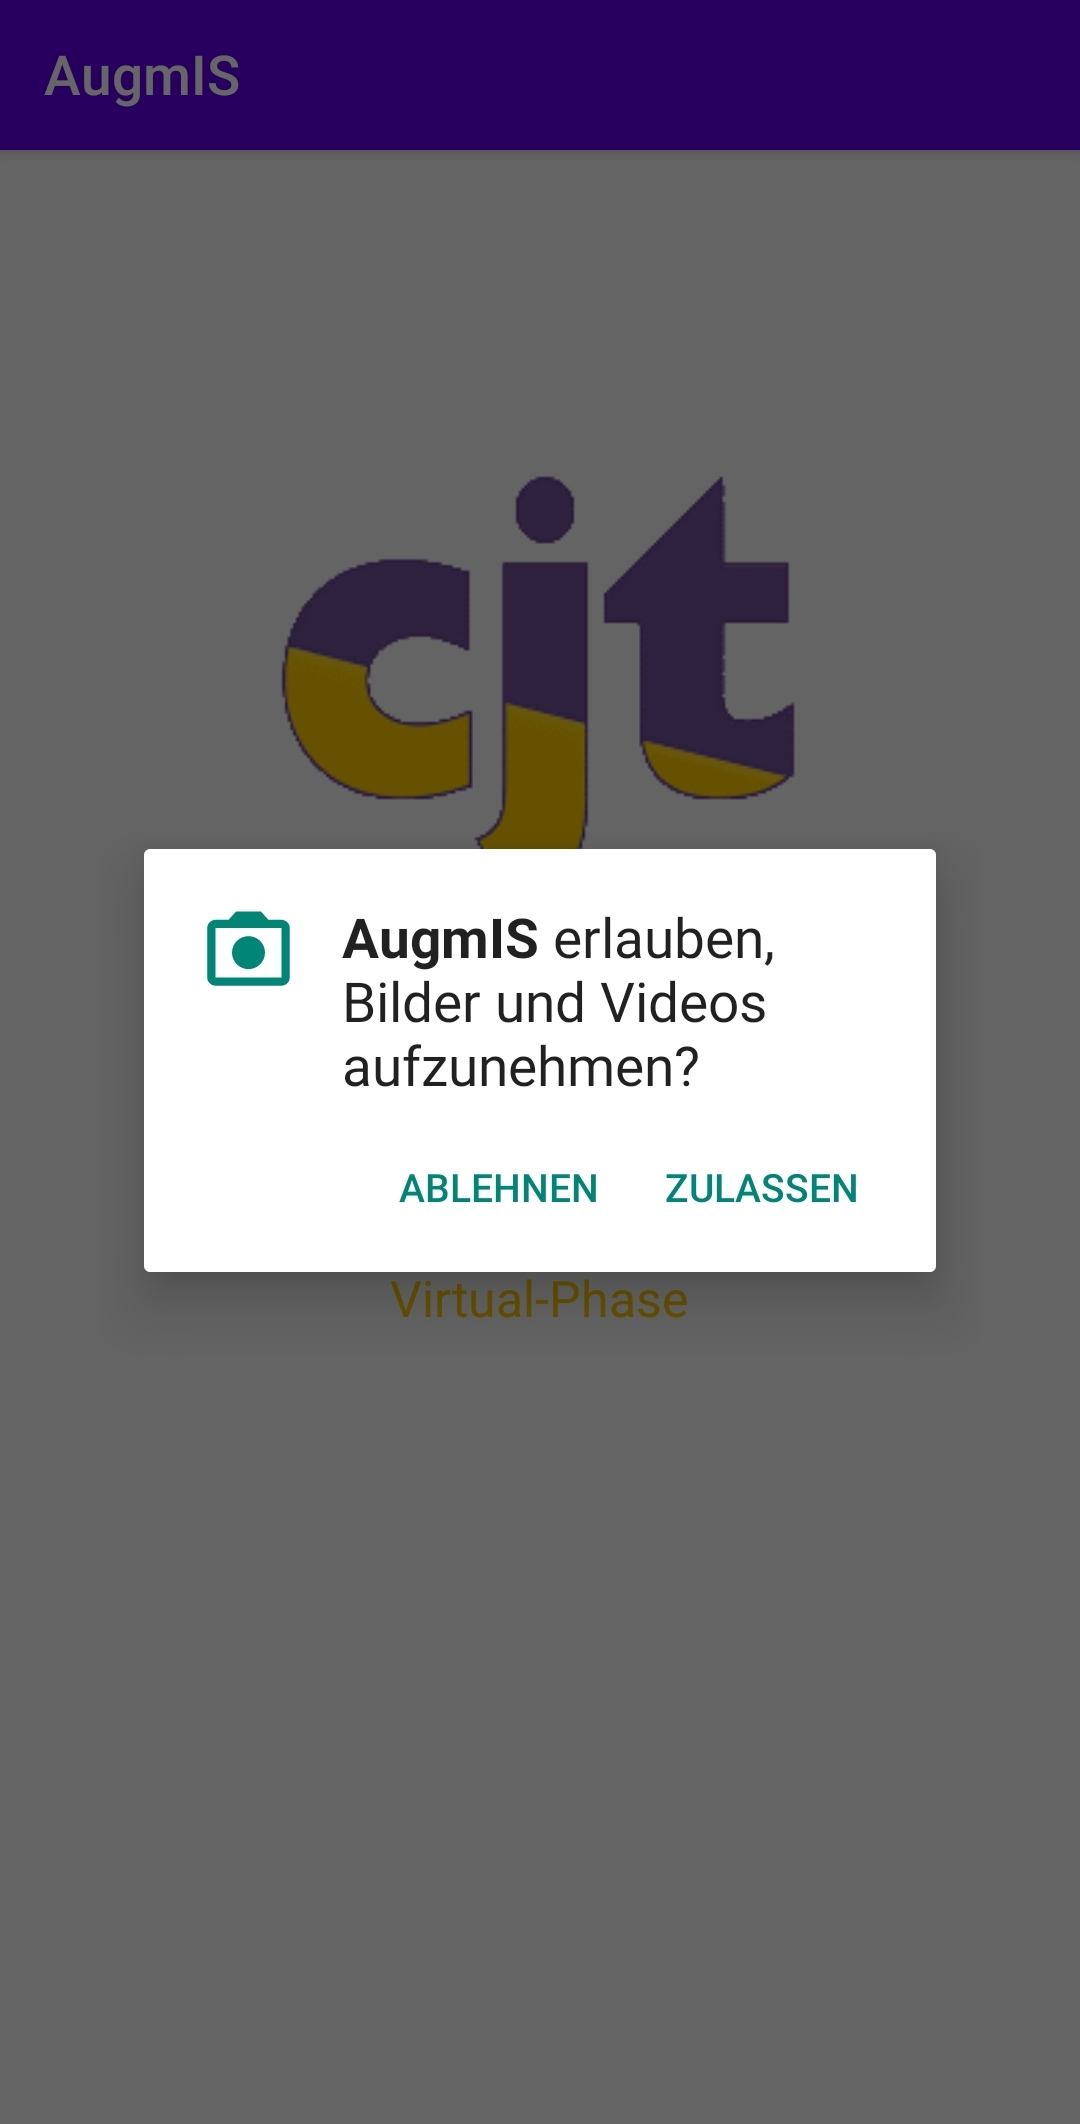
\includegraphics[width=10cm,height=7.5cm,keepaspectratio]{4Umsetzung/Bilder/camera_permission.jpg}
    \caption{Start der Applikation}
    \label{pic:camera_perm}
\end{figure}
\begin{figure}[hbt!]
    \centering
    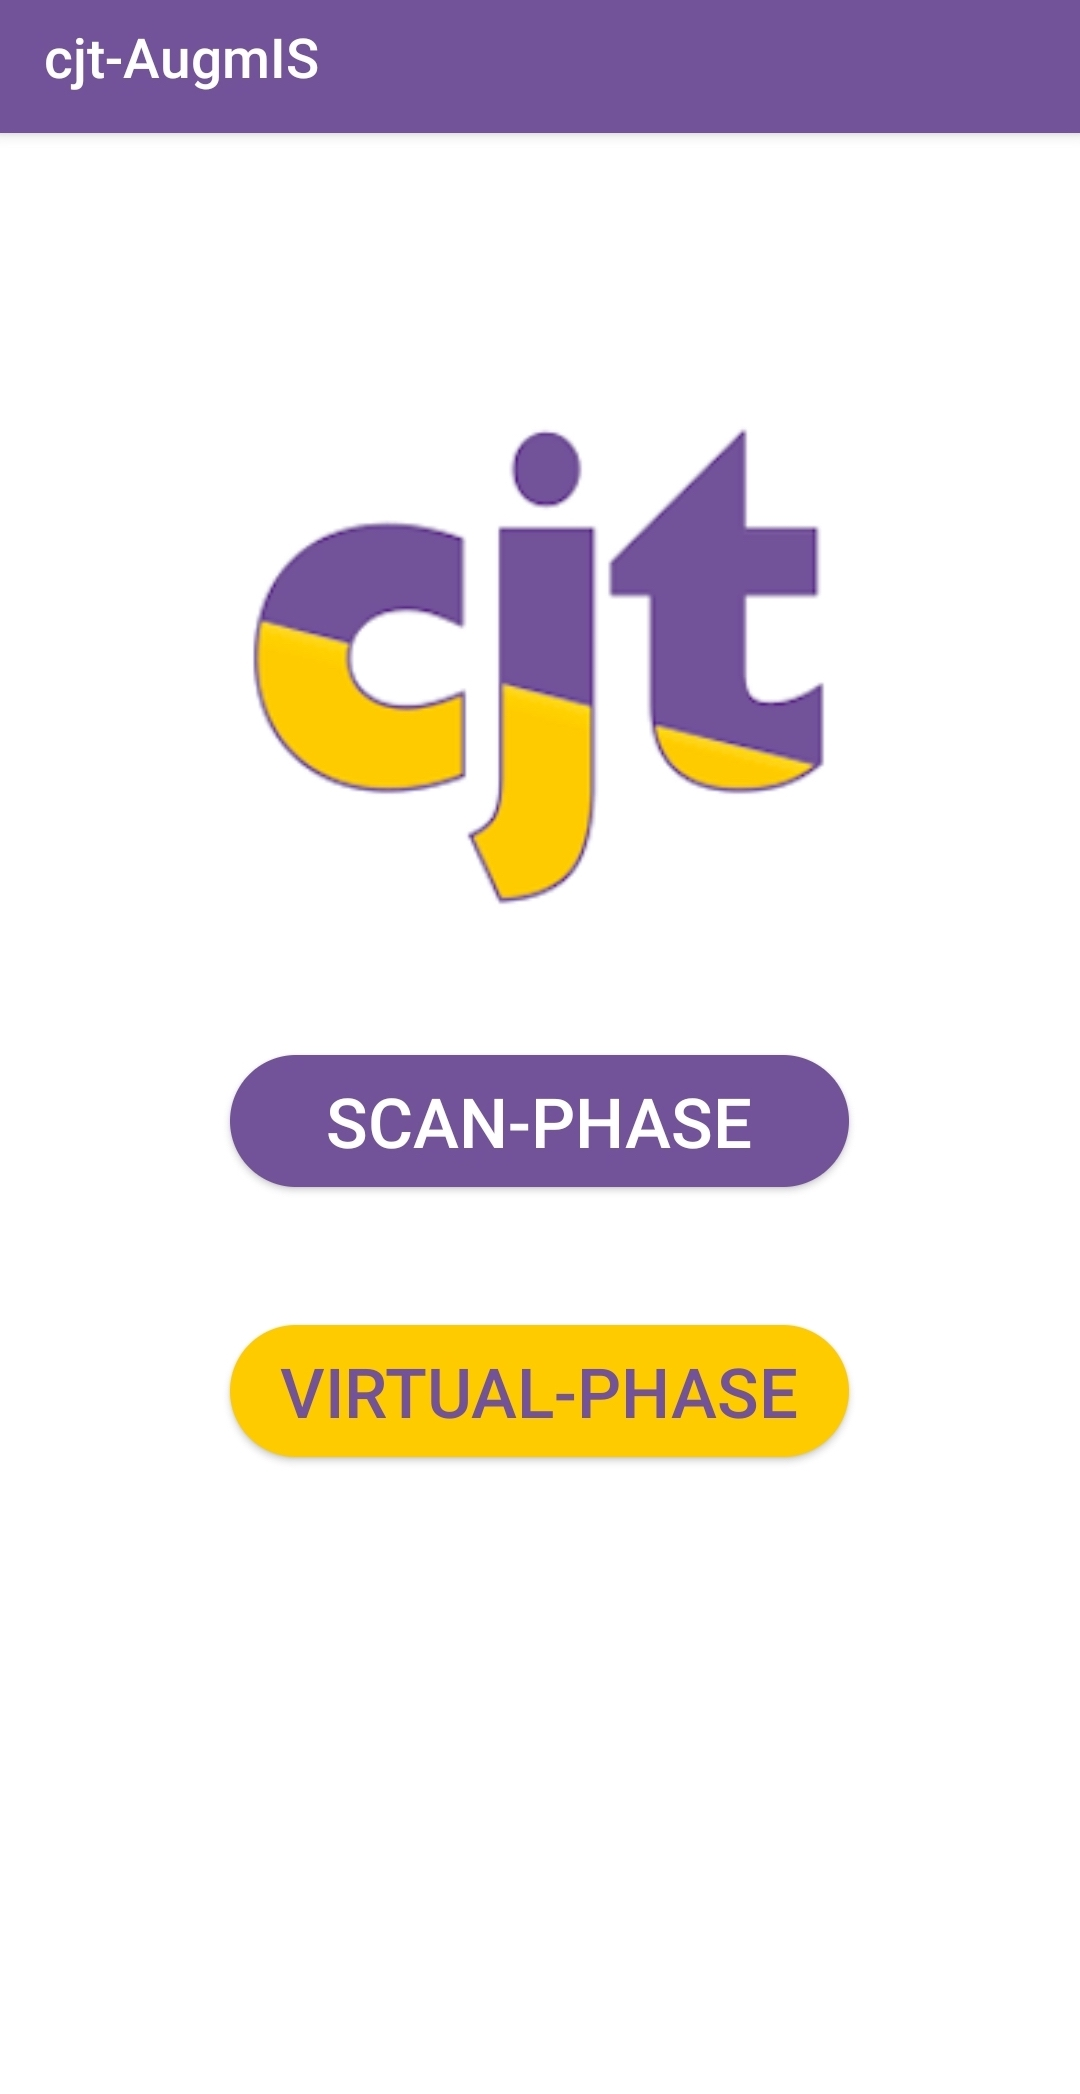
\includegraphics[width=10cm,height=7.5cm,keepaspectratio]{4Umsetzung/Bilder/startmenu.jpg}
    \caption{Startmenü der Applikation}
    \label{pic:startmenu}
\end{figure}
\subsubsection{BackEnd}

\subsection{Scan-Phase} %Umgebungserkennung /
\subsubsection{FrontEnd}
\begin{figure}[hbt!]
    \centering
    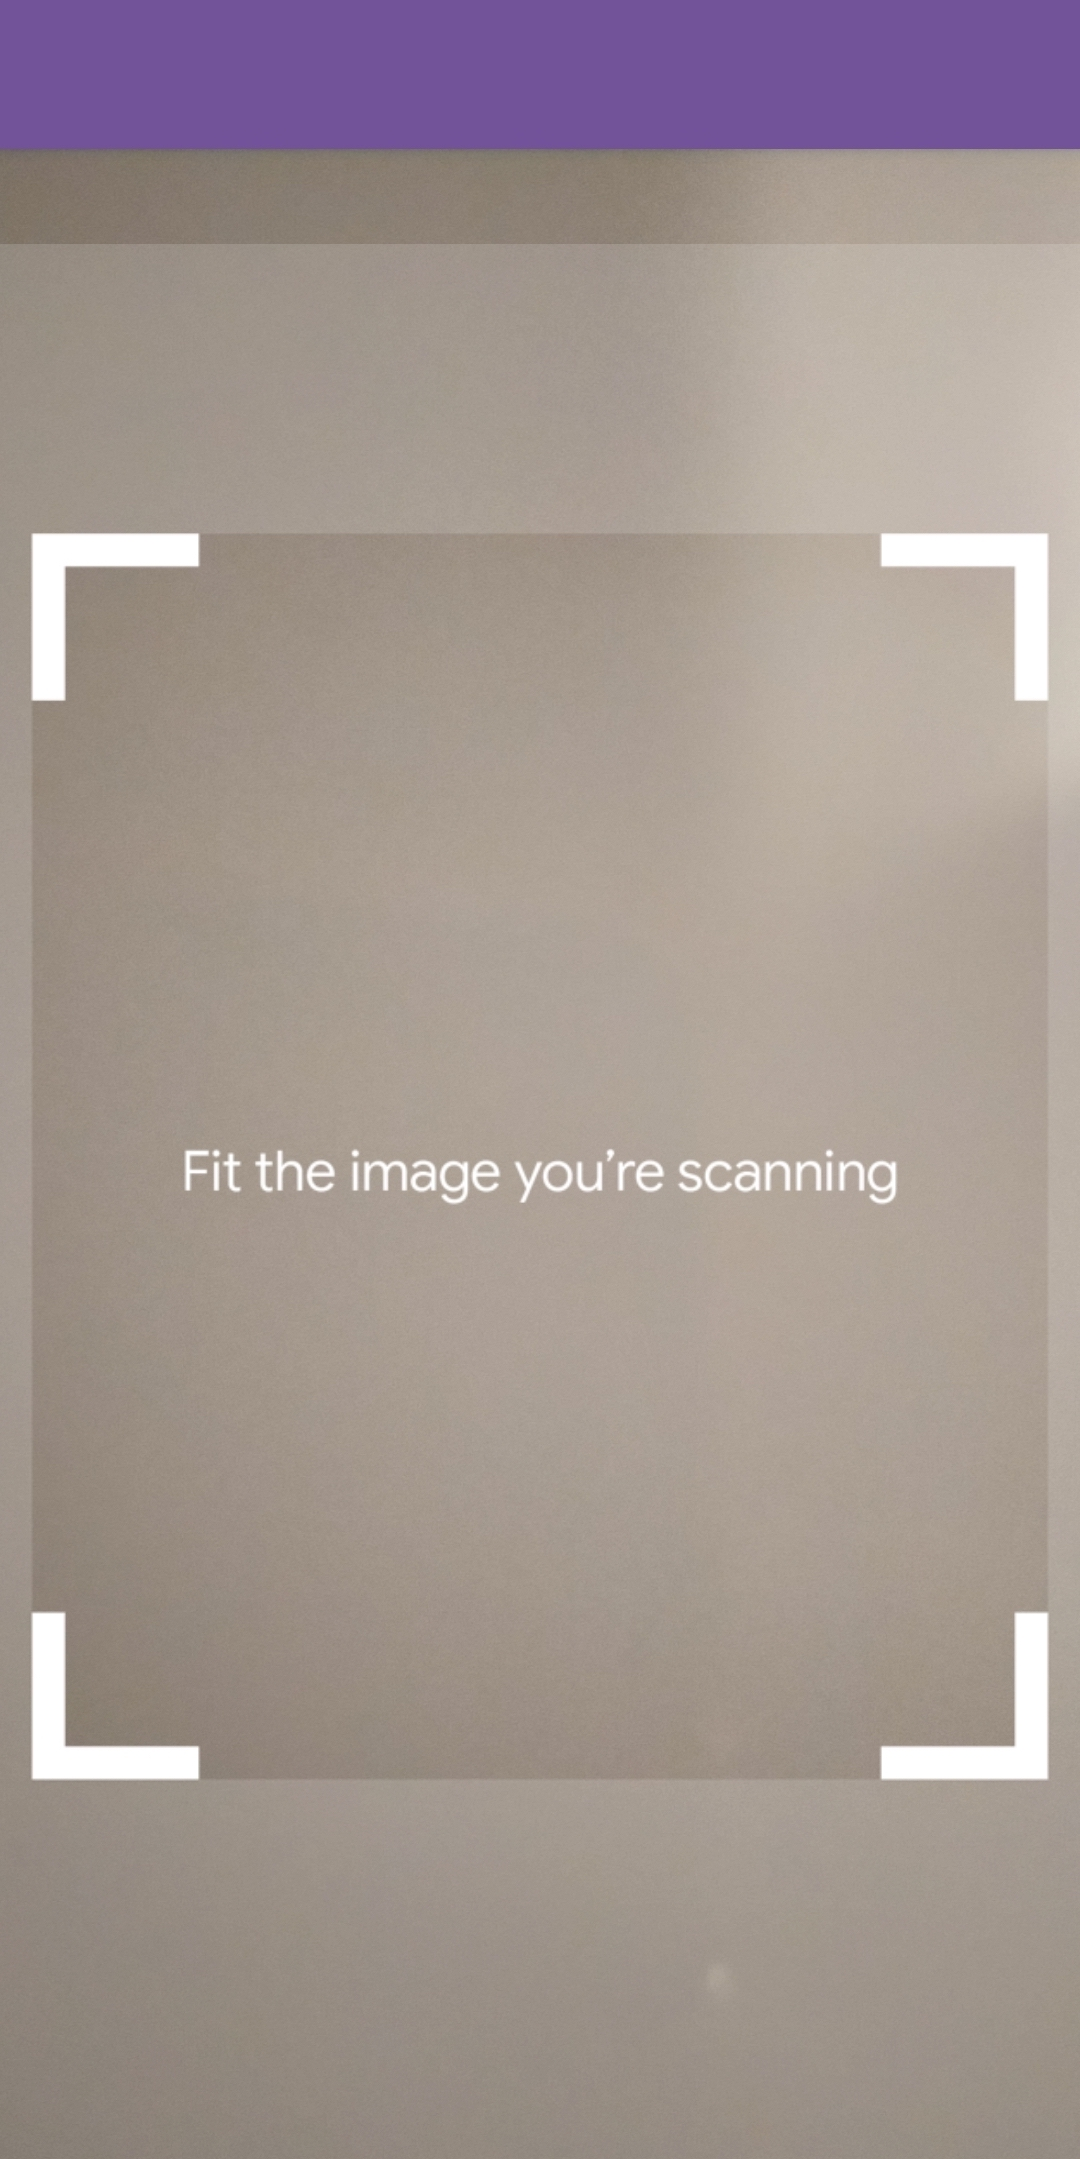
\includegraphics[width=10cm,height=7.5cm,keepaspectratio]{4Umsetzung/Bilder/image_tracking.jpg}
    \caption{Markererkennung der Applikation zum Start der Scan-Phase}
    \label{pic:image_tracking}
\end{figure}
\begin{figure}[hbt!]
    \centering
    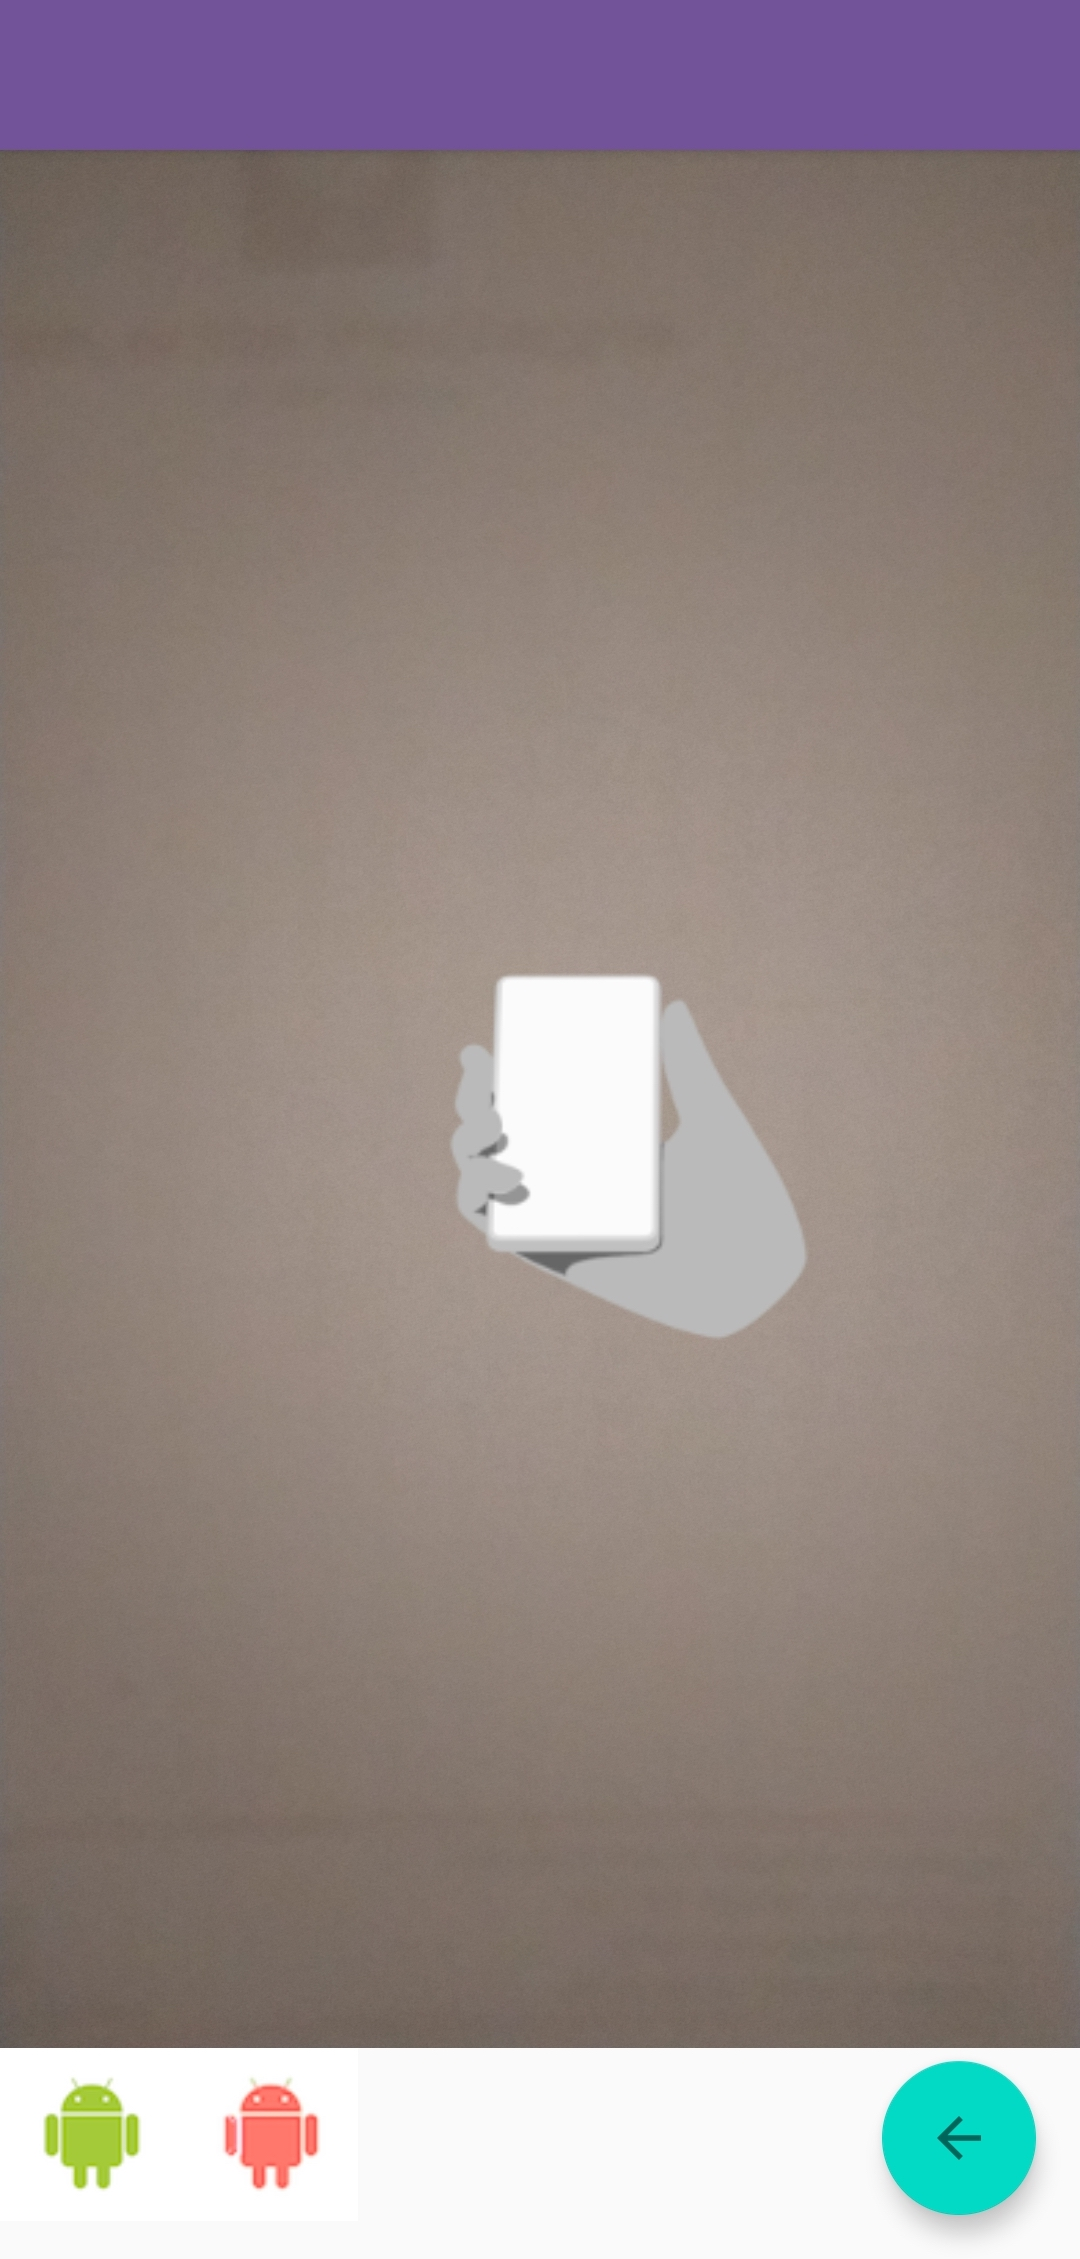
\includegraphics[width=10cm,height=7.5cm,keepaspectratio]{4Umsetzung/Bilder/scan-phase.jpg}
    \caption{Scan-Phase der Applikation}
    \label{pic:scan}
\end{figure}
\subsubsection{BackEnd}
\begin{figure}[hbt!]
    \centering
    
\includegraphics[width=5cm,height=5cm,keepaspectratio]{4Umsetzung/Bilder/cjt_logo_tracking.png}
    \caption{Marker zur Erkennung der Ausgangsposition}
    \label{pic:initialMarker}
\end{figure}

\subsection{Visualisierungs-Phase} 
\subsubsection{FrontEnd}
\begin{figure}[hbt!]
    \centering
    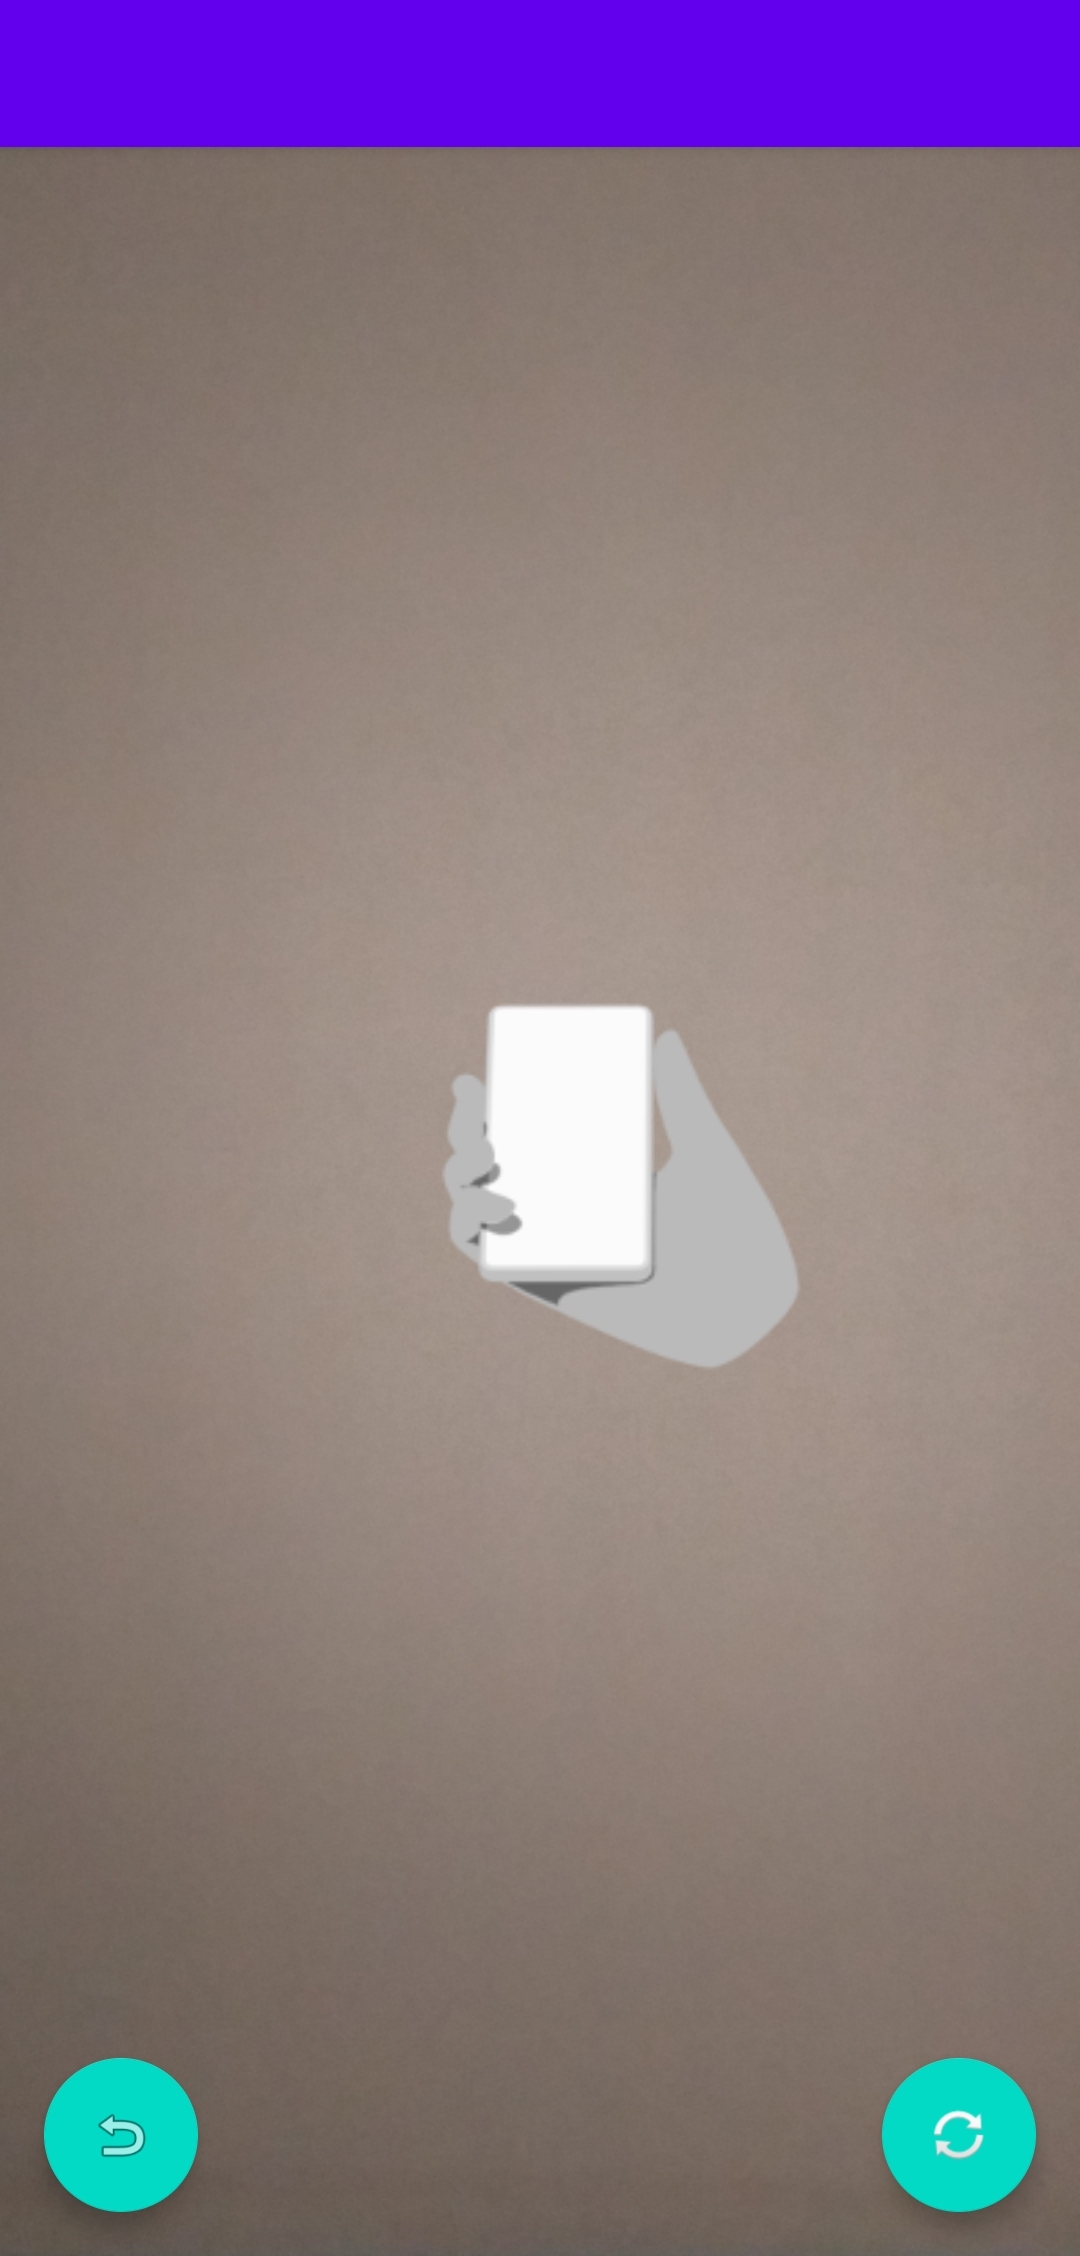
\includegraphics[width=10cm,height=7.5cm,keepaspectratio]{4Umsetzung/Bilder/visual-phase.jpg}
    \caption{Visualisierungs-Phase der Applikation}
    \label{pic:visual}
\end{figure}
\subsubsection{BackEnd}

\section{Testdurchlauf / Test-Szenario}
\label{chap:testdurchlauf}
\subsubsection{BackEnd}
Mit Beginn der Backend-Entwicklung wurden in erster Linie die Grundstrukturen implementiert, um der \textit{MVVM}-Architektur gerecht zu werden. Dabei lag 
der Fokus bei der Instanziierung der notwendigen Komponenten der \textit{Android Architecture Components}. Nach chronologischer Reihenfolge wurden die Klassen 
erstellt und mit den dazugehörigen Funktionen und Methoden versehen. Angefangen mit der Entity-Klasse zur Beschreibung des Objekts und deren allgemeiner Aufbau, 
dieser bereits in der Konzeption (\ref{chap:Konzeption}) unter dem Datenmodell (\ref{chap:Datenmodell}) festgehalten wurde. Darauffolgend wurde das „Data Object“ 
erstellt, welches die Zugriffe der Datenbankobjekte managed. Abschließend im Bereich der Datenbank ein Room-Layer, um die eigentliche Datenbank zu 
instanziieren und eine Zugriffsschicht auf die diese zu implementieren. 
\\ 
Zur Modularisierung und zur Generierung einer Schnittstelle für den Bezug zu mehreren Datenbeziehungspunkten wurde ein Repository erstellt, das eine saubere 
\acs{API} für den Datenzugriff auf den Rest der Anwendung bietet. Um die vorhandenen Klassen zum Datentransfer und zur Persistierung der Daten mit der 
eigentlichen Benutzeroberfläche zu verbinden, wurde ein ViewModel implementiert, welches die Daten zwischen den einzelnen Komponenten teilt und bereitstellt. 
\\ 
\linebreak 
Nach Aufzählung der einzelnen Bestandteile wird auf diese nun genauer eingegangen. 
\\ 
\linebreak
In einer Java-Klasse wird mithilfe der gegebenen Bibliothek „Room“ ein Entity-Objekt erstellt. Hierbei gibt es eine eindeutige Annotation, die die Klasse und 
deren beinhalteten Variablen deklariert. So wird, dem folgend aufgeführten Code-Beispiel (\ref{code:entity}) zu entnehmen, eine Klasse in eine Entity und somit 
in eine Datenbank-Tabelle konvertiert. In dieser Tabelle, definiert als \textit{„object\_table“}, gibt es weitere Variablen, die mit Annotationen versehen sind. 
Damit werden diese gemäß der Anforderungen des Konzepts definiert. Diese Variablen repräsentieren die Attribute des Datenbankschematas und stellen die einzelnen 
Informations- , bzw. -Datenbankspalten dar. Zur Veranschaulichung die Initialisierung der \acs{ID}-Vergabe eines Objekts. Diese wird als \textit{„id“}-Spalte 
und ebenso als Primärschlüssel\footnote{Einmaliger und eindeutiger Wert einer Tabelle, bzw. eines Attributs, um dieses eindeutig zu kennzeichnen.}-Variable 
deklariert.
\\ 
\linebreak
\begin{lstlisting}[language=C,
    frame=lines,           % Ein Rahmen um den Code (single for box, lines for top and bottom)
    xleftmargin=\parindent,  % Rahmen link von den Zahlen
    style=algoBericht,
    label={code:entity},
    captionpos=b,           % Caption unter den Code setzen
caption={Entity Code zur Initialisierung der Objekte}]
@Entity(tableName = "object_table")
public class Object {
    @ColumnInfo(name = "id")
    @NonNull
    @PrimaryKey(autoGenerate = true)
    private int id;

    public int getId() { return this.id; }
    public void setId(int id) { this.id = id; }
    ... 
}
\end{lstlisting}
\pagebreak
Das mit der Entity-klasse kommunizierende Modul ist das \textit{„Data Object“}, welches als Interface angelegt wurde. Das „Object Dao“ verwendet ebenso die Bibliothek 
„Room“ und wandelt die Java-Klasse per Annotation in ein „Dao“ um, dieses beinhaltet hauptsächlich die SQL-Queries zur Datenabfrage der vorhandenen Informationen. 
\\
\linebreak
\begin{lstlisting}[language=C,
    frame=lines,           % Ein Rahmen um den Code (single for box, lines for top and bottom)
    xleftmargin=\parindent,  % Rahmen link von den Zahlen
    style=algoBericht,
    label={code:query},
    captionpos=b,           % Caption unter den Code setzen
caption={SQL-Query zur Abfrage der Objekt-Namen}]
@Query("SELECT * FROM object_table ORDER BY name")
LiveData<List<Object>> getObjectName();
\end{lstlisting}
Anschließend nachdem die beiden Klassen erstellt waren, wurde das Datenbank-Layer auf der eigentlichen Datenbank implementiert. Über einen „Builder“ wird die 
Datenbank-Instanz erzeugt und mit einem Namen versehen. Im Fall des Assistenzsystems als \textit{„object\_database“} deklariert. 
\\ 
In zukünftiger Entwicklungen, 
falls notwendig, gäbe es die Möglichkeit in diesem Schema weitere Datenbanken zu erstellen und diese über weitere „Dao“s zu referenzieren. Darüber hinaus ist die 
Möglichkeit gegeben weitere Datenbank-Tabellen zu erstellen, um weitere Objekte und Informationen speichern zu können. Ebenso ist durch ein Repository die Option 
geboten, die derzeit auf dem Smartphone gespeicherte Datenbank auf einen externen Server auszulagern, um so die Daten weitläufiger zur Verfügung zu haben. 
Eine Datenbeziehung von generierten Daten der Maschinen und Geräte selbst wäre unter anderem auch vorstellbar, allerdings müssten diese vorab noch aufbereitet 
und zur Nutzung bereitgestellt werden. Diese Methode wird allerdings nicht näher betrachtet, da diese nicht teil dieser Arbeit ist. 
\\ 
Im Ausblick (\ref{chap:Ausblick}) wird darauf nochmals eingegangen.
\\ 
\linebreak
\begin{lstlisting}[language=C,
    frame=lines,           % Ein Rahmen um den Code (single for box, lines for top and bottom)
    xleftmargin=\parindent,  % Rahmen link von den Zahlen
    style=algoBericht,
    label={code:dblayer},
    captionpos=b,           % Caption unter den Code setzen
caption={Erzeugung des Datenbank-Layers „Room“}]
@Database(entities = {Object.class}, version = 1, exportSchema = false)
public abstract class ObjectRoomDatabase extends RoomDatabase {
    ...
    INSTANCE = Room.databaseBuilder(context.getApplicationContext(),
    ObjectRoomDatabase.class, "object_database")
    .addCallback(sRoomDatabaseCallback)
    .build();
    ...
}
\end{lstlisting}
Letzter wichtiger zu implementierender Aspekt war das Kommunikations-Modul zwischen den Datenbank-Transfers und der Benutzeroberfläche, das ViewModel. 
In dieser Klasse wird eine Liste erstellt, welche den Wert des zu speichernden Objekts besitzt. Diese werden über eine „get“-Funktion aus dem zuvor 
instanziierten Repository geladen und in der erzeugten Liste lokal abgelegt. Diese Liste wird dann für die Präsentation der Informationen auf der 
Nutzeroberfläche verwendet. 
\\ 
\linebreak
Ursprünglich war die Implementierung der eigentlichen Scan-Phase unter Beachtung der ARCore-\acs{API} einfach angedacht, die sich im Laufe der Entwicklung 
allerdings als nicht so praktikabel herauskristallisierte. Diese aufgetretene Problemstellung wird in weiterem Verlauf präzisiert, nachdem der eigentliche 
Verlauf geschildert wurde. 
\\ 
Das Fragment auf dem \acl{UI} der Scan-Phase (\ref{pic:scan}) wird als \acs{AR}-Fragment, unter der Benutzung des Sceneform \acs{SDK}s, deklariert. Basierend auf 
dieser Initialisierung können die Interaktionen mit den ARCore-, bzw. Sceneform- Elementen gewährleistet werden. Dadurch ist ebenso die Nutzung der Kamera 
gegeben. Diese Funktionen sind Bestandteile der ARCore- und Sceneform-\acs{API}. Über einen \textit{„FragmentManager“} wird die „.xml“-Datei mit dem darin 
enthaltenen Fragment der ID \textit{„sceneform\_fragment“} initialisiert.
\\
\begin{lstlisting}[language=C,
    frame=lines,           % Ein Rahmen um den Code (single for box, lines for top and bottom)
    xleftmargin=\parindent,  % Rahmen link von den Zahlen
    style=algoBericht,
    label={code:arfragment},
    captionpos=b,           % Caption unter den Code setzen
caption={Initialisierung des Fragments}]
private ArFragment fragment;
...
fragment = (ArFragment)
getSupportFragmentManager().findFragmentById(R.id.sceneform_fragment);
...
\end{lstlisting}
Um anschließend Objekte auf diesem Fragment einblenden zu können, ist es vorab notwendig eine \textit{„Session“} zu generieren, die unter anderem für die 
Konfigurationen der Kamera zuständig ist. Dadurch wird bei Start der Scan-Phase ein dreidimensionales Koordinatensystem erstellt, welches den Ursprungspunkt der 
Anwendung darstellt. Mit Verwendung der internen Sensoren des Smartphones werden darauffolgende Bewegungen registriert und mittels \acs{SLAM} Verfahren berechnet. 
So ist die Kalkulation der Lokalisation möglich und anhand der Kamera kann auf Basis des \acs{SLAM} Verfahrens die Umgebung abgebildet werden. Durch diese 
Gegebenheiten wird die virtuelle Karte des Umfelds erzeugt und dient so zur Veranschaulichung der zu platzierenden Objekte. In der Abbildung (\ref{pic:koordin}) 
ist ein Beispiel zu sehen, indem ein Objekte erstellt wird, welches die Koordinaten von dem Ursprungspunkt berechnet. So wird deutlich, wie die Position eines 
Objekts errechnet wird, unter der Verwendung des von ARCore gegebenen \acs{SLAM} Verfahrens. Vorausgesetzt der Anwender startet an der Position (x,y,z = 0), 
bewegt sich frei im Raum und setzt an Postion (x = 5, y = 1, z = 3.5) ein Objekte.
\begin{figure}[hbt!]
    \centering
    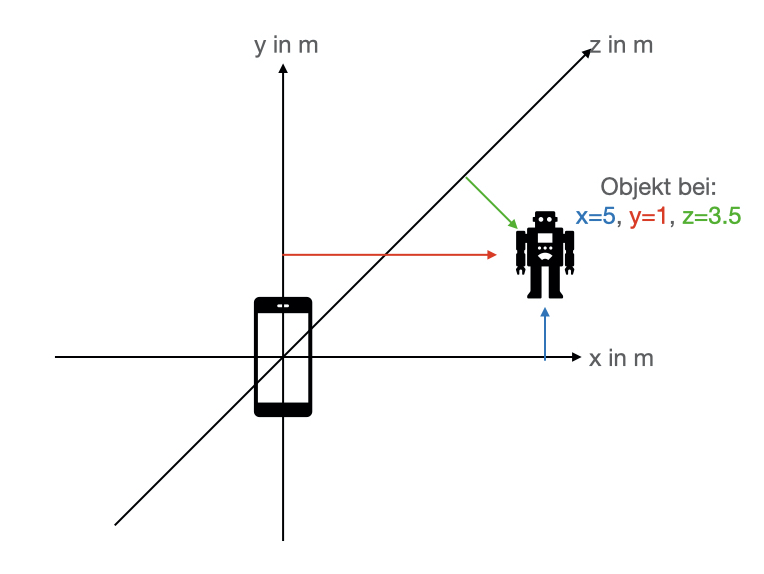
\includegraphics[width=10cm,height=10cm,keepaspectratio]{4Umsetzung/Bilder/koordin.jpeg}
    \caption{Aufbau der Positionsberechnung von Objekten}
    \label{pic:koordin}
\end{figure}
\\ 
Beim setzen eines Objekts wird als Anhaltspunkt der Mittelpunkt des Bildschirms berechnet, um das Objekt zentriert platzieren zu können. Ist 
diese Position berechnet, ist durch Hilfe des \acs{SLAM} Verfahrens die genaue virtuelle Position zu ermitteln und anhand dieser ist das Objekt 
zu platzieren. 
\\ 
Das Objekte wird gesetzt, indem der Nutzer in der \acs{UI} (\ref{pic:scan}) im Bereich der „Gallery“ ein Objekt angeklickt.
Über die der Sceneform-\acs{API} zur Verfügung gestellte Methode („ModelRenderable“) wird das Objekt erstellt und als „Anchor“ auf die berechnete Position 
gesetzt. Ein Anchor ist die fixe Position des Objekts, an dem dies platziert wird und so lange dort vorhanden bleibt, bis die Applikation beendet wird. Die Datei 
die als dreidimensionales asset genereirt werden soll, wird über die „uri“-Variable übergeben. 
\begin{lstlisting}[language=C,
    frame=lines,           % Ein Rahmen um den Code (single for box, lines for top and bottom)
    xleftmargin=\parindent,  % Rahmen link von den Zahlen
    style=algoBericht,
    label={code:modelrenderable},
    captionpos=b,           % Caption unter den Code setzen
caption={ModelRenderable Builder}]
ModelRenderable.builder()
.setSource(owner.get(), uri)
.build()
.handle((renderable, throwable) -> {
    ...
}
\end{lstlisting}
Während der Objekt-Renderung öffnet sich die \acs{GUI} (\ref{pic:createObject}) zur Eingabe der Informationen, die sich auf das Objekt beziehen. Diese 
werden dann zusammen mit der virtuellen Position des Objekts abgegriffen und in die Datenbank geschrieben. Drückt der Anwender den „save“-Button der Oberfläche 
beendet er diesen Vorgang und kehrt auf die \acs{UI} der Scan-Phase zurück, um weiter Objekte platzieren zu können. 
\\ 
Zu der Position des Objekts wird dessen Rotation durch die einfache Berechnung durch Quaternionen ebenso in die Datenbank gespeichert, um die Darstellung so real 
wie möglich wiederzugeben. Damit erfolgt die Feststellung, dass das Objekt immer in Blickrichtung der Kamera positioniert ist, da die Rotation ausgehen von der 
Kamerahaltung berechnet wird. 
%--> Problemschilderung der Speicherung der Session
\\ 
\linebreak
Ursprünglich war geplant, die generierte Session sowie die darin erstellten Objekte in der Datenbank abzuspeichern, um diese bei erneutem Aufruf der 
Scan-Phase, bzw. bei Anwendung der Visualisierungs-Phase zu laden und innerhalb der Session wieder anzeigen zu lassen. Da die Datenbank nur gewisse Datentypen 
zulässt, war das erste auftretende Problem die Speicherung der Session als Objekt, welches zunächst in eine „BLOB“-Datei konvertiert wurde, um diese speichern 
zu können. Eine „BLOB“-Datei ist ein Binary Large Object, welches anhand der Binärcodierung abgespeichert wird. Dabei kann es sich unter anderm um große 
Bild- oder Audio-Dateien handeln, auch können so anderweitig große Dateien gespeichert werden. Mit dieser Umsetzung tat sich auch schon das nächste Problem auf, 
welches deutlich schwerwiegender war und auch in diesem Sinne die Visualisierungs-Phase betraf. 
\\ 
Da eine erzeugte Session nur eine gewissen Zeit verwendet wird, ist diese für den weitern Gebrauch nicht vorgesehen, dies bedeutet, dass nach erneutem Starten 
des Assistenzsystems alle zuvor erzeugten Objekte zwar auf die dazugehörige Session bestimmt sind, allerdings auf der zugewiesenen Position 
nicht mehr erreichbar wären. Durch die Unterschiedlichen Startpunkte, die bei wiederholtem Starten der Anwendung erzeugt worden würden, 
würde sich die ursprüngliche Ausgangsposition der Applikation verschieben und so auch die Objekte an eine fälschliche Position projizieren. Somit wäre das 
Ergebnis nicht exakt und könnte keine Anwendung finden, da die Applikation Informationen anzeigen würde, die der Realität nicht entsprechen. 
\\ 
Basierend auf dieser Erkenntnis musste umdisponiert und ein neuer Lösungsansatz konzipiert werden. Mit dem Wissen über den aktuellen Stand der ARCore \acs{API} 
war es die neue Aufgabe eine Lösung zu entwickeln, welche exakt und zuverlässig arbeitet, um keine falschen Informationen wiederzugeben. 
\\ 
Dieser Ansatz wird nun erläutert.
\\ 
\linebreak
Die Idee war es, einen Fixpunkt zu erstellen, welcher dazu diente einen immer gleichbleibenden Startpunkt zu setzen. Dadurch gäbe es keine Unterschiede des 
Ausgangspunktes mehr und der Nutzer könnte trotz seiner aktuellen Position starten. Dazu müsste er beim Start der Applikation an den Ursprungspunkt kehren, 
um daraufhin die Funktion starten zu können. Für diesen Ansatz wurde ein Marker gewählt (siehe Abbildung \ref{pic:initialMarker}) der vor dem ersten Gebrauch 
der Software an einer Position angebracht wird und an dieser bleibt. 
\begin{figure}[hbt!]
    \centering
    
\includegraphics[width=5cm,height=5cm,keepaspectratio]{4Umsetzung/Bilder/cjt_logo_tracking.png}
    \caption{Marker zur Erkennung der Ausgangsposition}
    \label{pic:initialMarker}
\end{figure}
\\
Um diesen Ansatz umsetzen zu können, musste eine weitere Funktion zur Applikation hinzugefügt werden (siehe Abbildung \ref{pic:image_tracking} 
in Scan-Phase \ref{chap:scan_implementation} Frontend), damit ein Marker verfolgt werden kann. Wird dieser Marker erkennt folgt die eigentliche Scan-Phase 
die daraufhin bei der Objektplatzierung und Datenspeicherung ebenso umgewandelt wurde. 
%--> Ablauf nach Markererkennung inkl. Berechnung und speicherung der Positionsdaten.

Ausgehend von dem Marker wird dann die Funktion zur Verfolgung des Markers gestartet

\begin{figure}[hbt!]
    \centering
    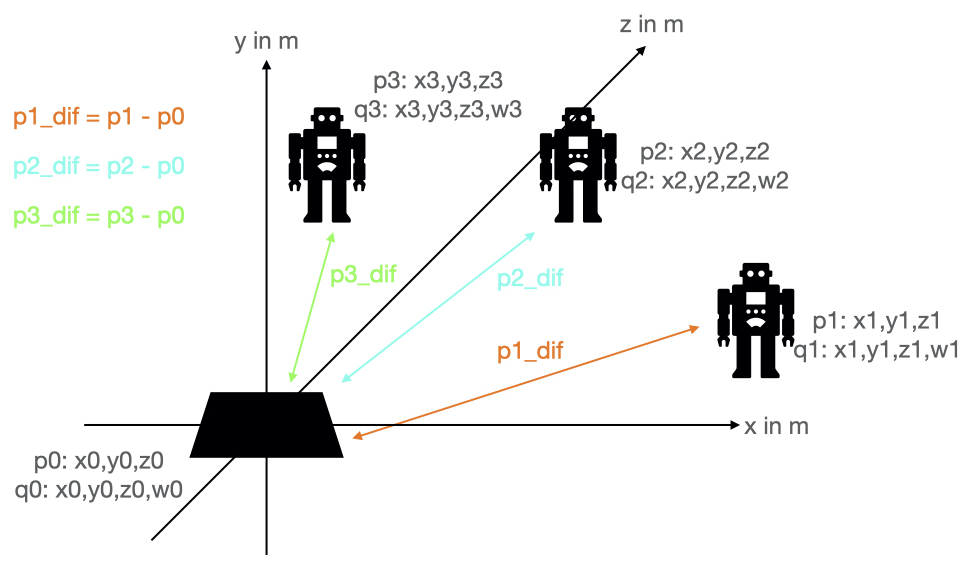
\includegraphics[width=15cm,height=15cm,keepaspectratio]{4Umsetzung/Bilder/difcalc.jpeg}
    \caption{Positionsberechnung zum Ursprungsmarker}
    \label{pic:differenztoinitial}
\end{figure}


\subsubsection{BackEnd}
Nachdem das Problem der variablen Startposition in der Implementierung der Scan-Phase umgangen wurde, konnte die Visualisierungs-Phase entwickelt werden. 
\\ 
\linebreak
Wählt der Anwender auf der Startmenü-\acs{UI} (\ref{pic:startmenu}) den Button „Virtual-Phase“, wird eine Anmerkung getätigt, indem der Nutzer darüber in 
Kenntnis gesetzt wird, dass er zu Beginn die Scan-Phase durchgeführt haben muss, bevor die Visualisierungs-Phase gestartet werden kann. Diesen Vermerk kann der 
Benutzer ignorieren, wenn dieser weiß, dass ein Scan durchgeführt wurde, oder er akzeptiert den Hinweis und wird auf die dementsprechende Funktion weitergeleitet. 
Der Nutzer wird dadurch davor bewahrt, eine Funktion starten zu wollen, die ohne Inhalt keine Änderungen aufzeigt.
\\ 
Danach wird der Nutzer aufgefordert, den initialen Marker (\ref{pic:initialMarker}) einzuscannen, um die ursprüngliche Position, bzw. die Markierung festzuhalten. 
Damit kann der weitere Programmablauf folgen, indem die \acs{GUI} der Visualisierungs-Phase (\ref{pic:visual}) angezeigt und eine neue Session zur 
Objektplatzierung gestartet wird. 
\\
Über eine ViewModel-Komponente werden die Objekte aus der Datenbank abgefragt und in einer Liste gespeichert, um diese zu einem späteren Zeitpunkt zur Platzierung der 
Objekte verwenden zu können. 
\\ 
Ist der Marker erkannt worden, wird mithilfe des Buttons, der sich im rechten unteren Eck der Benutzeroberfläche (\ref{pic:visual}) befindet, die Methode zur 
Datenabfrage, Erzeugung und Platzierung der Objekte gestartet. Dabei wird über den Button-Klick eine Funktion aufgerufen, die die Liste der Objekte anspricht und 
die jeweils darin enthaltenen Objekte nacheinander generiert. Nach Betätigen des Buttons ist dieser auf der \acs{UI} nicht mehr aufzufinden, um einer weiteren 
Platzierung aller Objekte vorzubeugen. Die von dem ViewModel gegebene Liste wird, abhängig von deren Länge, iterativ abgearbeitet und die Objekte 
nacheinander angelegt. Dies erfolgt über eine „for“-Schleife, welche abhängig von dem Ursprungspunkt, dem Marker „objectMarkerCenter“, die Position des 
aktuellen Objekts „obj“ an der Stelle „i“ in der Liste neu errechnet und darstellt.
\\ 
\linebreak
\begin{lstlisting}[language=C,
    frame=lines,           % Ein Rahmen um den Code (single for box, lines for top and bottom)
    xleftmargin=\parindent,  % Rahmen link von den Zahlen
    style=algoBericht,
    label={code:listOfObjects},
    captionpos=b,           % Caption unter den Code setzen
caption={Abfolge der Objekte in der Liste}]
... 
for (int i = 1; i < listOfObj.size(); i++){
    obj = listOfObj.get(i);
    if(!obj.getName().equals("origin")) {
        calculateObjectPosition(obj, i, objectMarkerCenter);
    }
}
\end{lstlisting}
Mit der gegebenen „calculateObjectPosition“ wird dann die Distanz vom Ursprungsmarker zu dem Objekt addiert, um 
die Positionen und Distanzen der einzelnen Objekte der Scan-Phase exakt wiederzugeben. Ist die Addition zu einem Objekt durchgeführt, repräsentiert diese 
Berechnung unabhängig von der Startposition des Anwenders die neue Position, an der das Objekt platziert werden muss. Somit ist der Nutzer bei Verwendung der 
Applikation in der Lage, aus einem vorab beliebigen Punkt zu starten und alle Objekte exakt auf die referenzierte, ursprüngliche Position zu setzen, die 
in der Scan-Phase festgelegt wurde. Nachdem die Position des aktuellen Objekts berechnet wurde, wird diese als neue „Pose“ initialisiert und übergeben, um 
das zu erstellende Objekt zu rendern und auf der Oberfläche anzuzeigen. Dabei findet eine Abfrage des Status statt, um daraufhin 
entscheiden zu können, in welcher Farbe das Objekt zu Präsentieren ist.  
\\ 
\begin{lstlisting}[language=C,
    frame=lines,           % Ein Rahmen um den Code (single for box, lines for top and bottom)
    xleftmargin=\parindent,  % Rahmen link von den Zahlen
    style=algoBericht,
    label={code:additionOfObject},
    captionpos=b,           % Caption unter den Code setzen
caption={Berechnung der Markerplatzierung}]
public void calculateObjectPosition
 (Object object, int i, Object objOrigin){
    ... 
    qx = object.getQx() + objOrigin.getQx();
    qy = object.getQy() + objOrigin.getQy();
    qw = object.getQw() + objOrigin.getQw();
    qz = object.getQz() + objOrigin.getQz();

    tx = object.getTx() + objOrigin.getTx();
    ty = object.getTy() + objOrigin.getTy();
    tz = object.getTz() + objOrigin.getTz();

    float[] rotation = {qx,qy,qz,qw};
    float[] translation = {tx,ty,tz};

    Pose pose = new Pose(translation, rotation);

    if(objectViewModel.getAllObjectsName()
     .getValue().get(i).getState() == 1) {
        addObject(Uri.parse("object.sfb"), pose, i);
    }

    if(objectViewModel.getAllObjectsName()
     .getValue().get(i).getState() == -1){
        addObject(Uri.parse("object_red.sfb"), pose, i);
    }
}
\end{lstlisting}
Sind alle Listenelemente abgearbeitet, ist die Erstellung und Renderung der Objekte fertig. Danach werden dem Nutzer alle vorhandenen Objekte angezeigt und 
visualisiert. Mit diesen Erkenntnissen kann der Nutzer durch den Raum laufen und alle Objekte überwachen. Wird ein Objekt anvisiert, kann über eine Berührung 
des Objekts auf dem Display alle vorhandenen Informationen eingesehen werden. Somit sind die Informationen des einzelnen Objekts schnell sichtbar.  
Die Applikation kann beliebig oft geschlossen und neu gestartet werden. Der Nutzer kann sich zu jeder Zeit die Objekte visualisieren lassen, vorausgesetzt, der 
Ursprungsmarker wird zu Anfang eingescannt. Daraufhin können alle Objekte präsentiert und die dazugehörigen Informationen angezeigt werden. %  zu jeder Zeit
\\ 
\linebreak
Um die soeben beschriebene Backend-Implementierung der Visualisierungs-Phase zu demonstrieren, wird diese anhand eines kleinen Szenarios veranschaulicht. 
\\ 
Startet der Nutzer die Visualisierungs-Phase, muss er den initialen Marker scannen, um fortfahren zu können. Darauffolgend öffnet sich die \acs{GUI} dieser 
Phase und mit einem Klick auf den Button rechts unten auf der Oberfläche synchronisiert er die Funktion und alle Objekte, die in der Scan-Phase gesetzt wurden, 
werden erneut generiert. Daraufhin kann der Nutzer die Objekte an den Stellen einsehen, an denen sie sich ursprünglich befanden. So werden diese samt Status 
angezeigt und der Nutzer hat den gesamten Überblick über alle Objekte und kann diese beobachten. Der Schritt ist der Abbildung (\ref{pic:visual_objects}) 
zu entnehmen. 
\begin{figure}[hbt!]
    \centering
    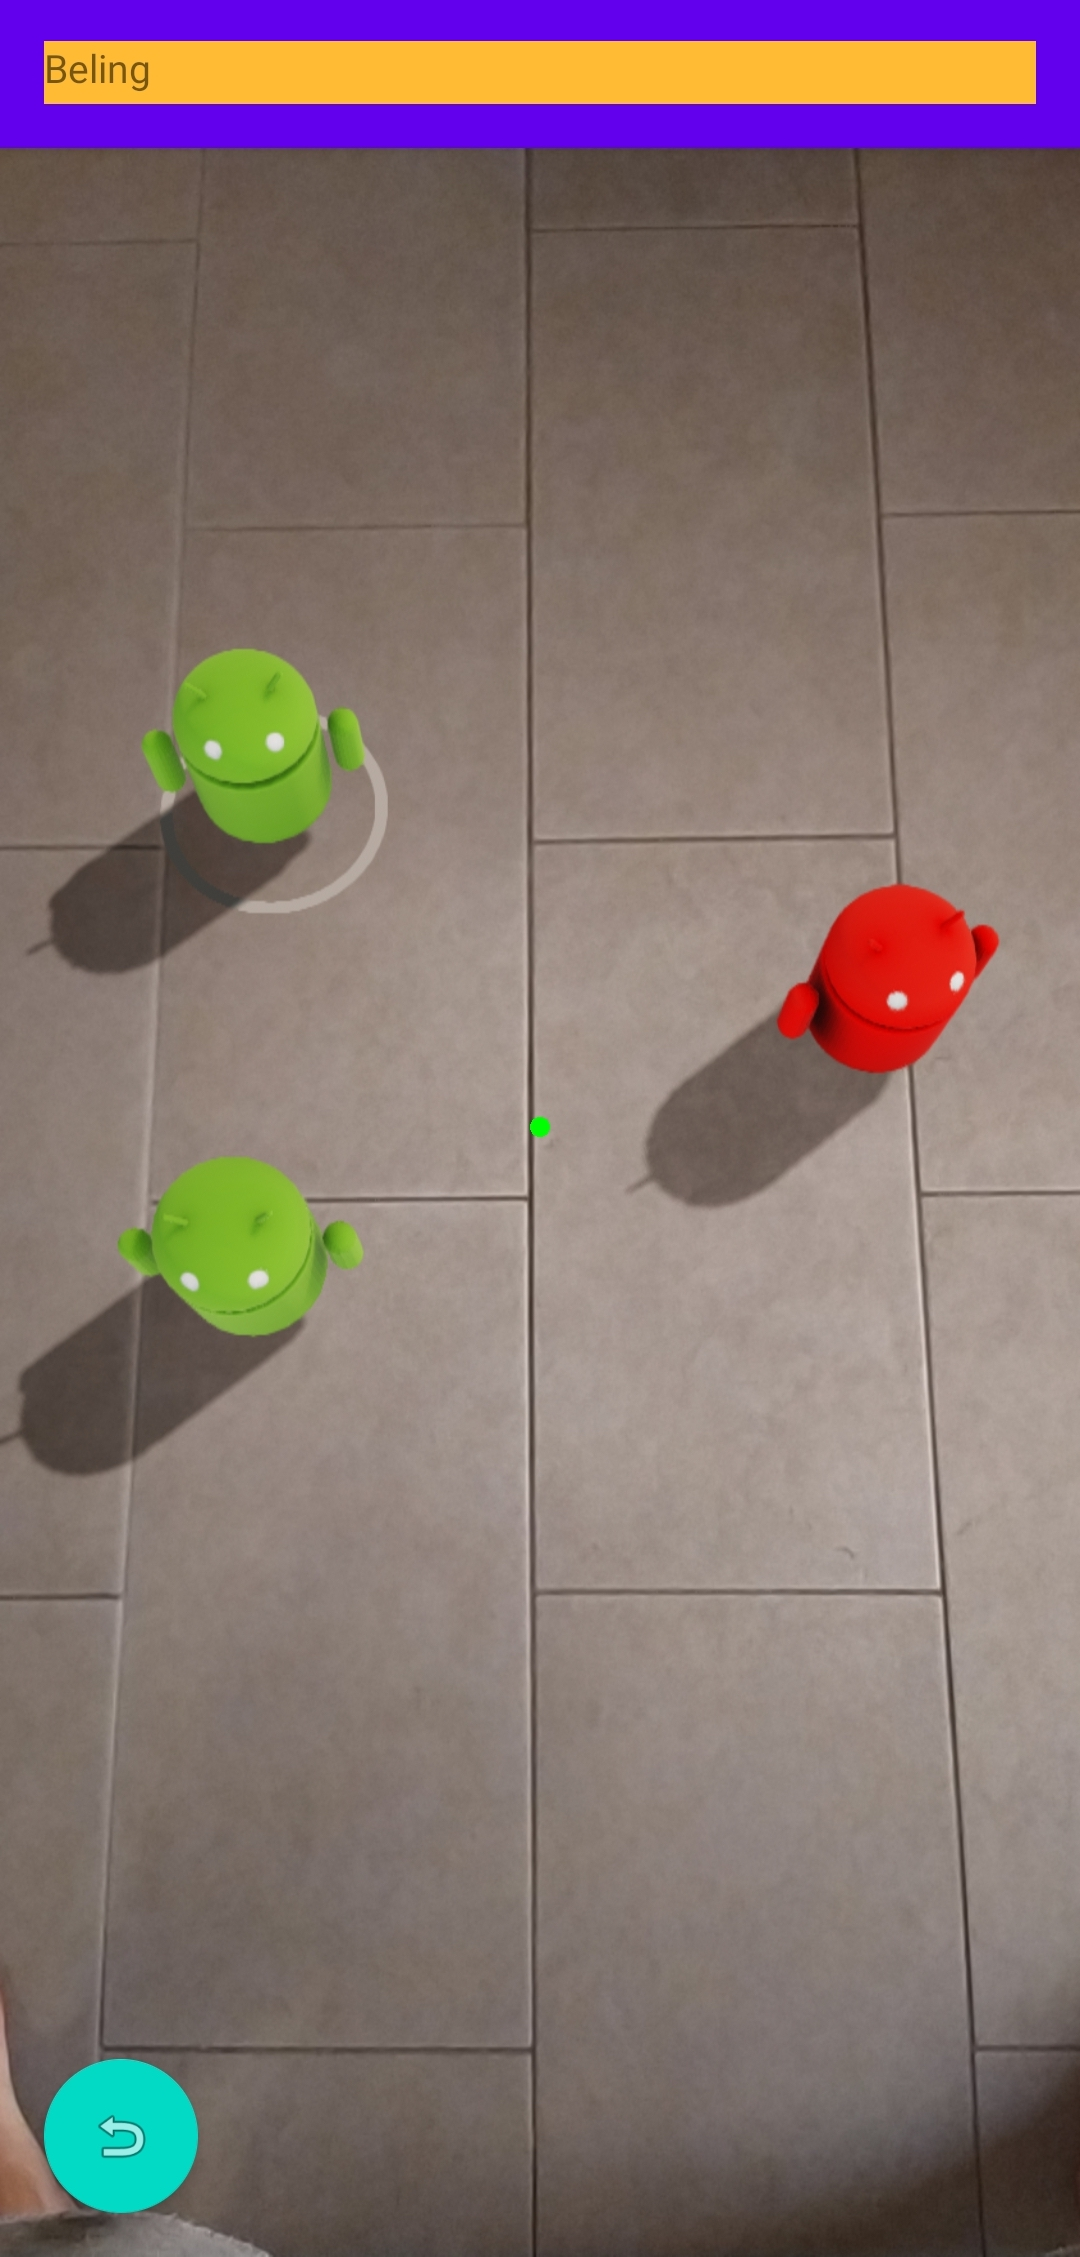
\includegraphics[width=10cm,height=7.5cm,keepaspectratio]{4Umsetzung/Bilder/show_objects_after_loading.jpg}
    \caption{Funktion Visualisierungs-Phase Teil 1}
    \label{pic:visual_objects}
\end{figure}
\\ 
\linebreak
Eine weiter Funktion dieser Phase ist die Verwaltung der Objekte und deren Informationen. Wird ein Objekt anvisiert, werden mit einem Klick auf das Objekt 
die Informationen über ein PopUp angezeigt. Darunter ist der Namen des Objekts, der Status und die ID, die zu Anfang automatisch generiert 
und vergeben wurde. So kann zu jedem einzelnen Objekt dessen Informationen zur Verfügung gestellt werden. 
\pagebreak
\begin{figure}[hbt!]
    \centering
    \subfigure[Anzeige der Objektinformationen 1]{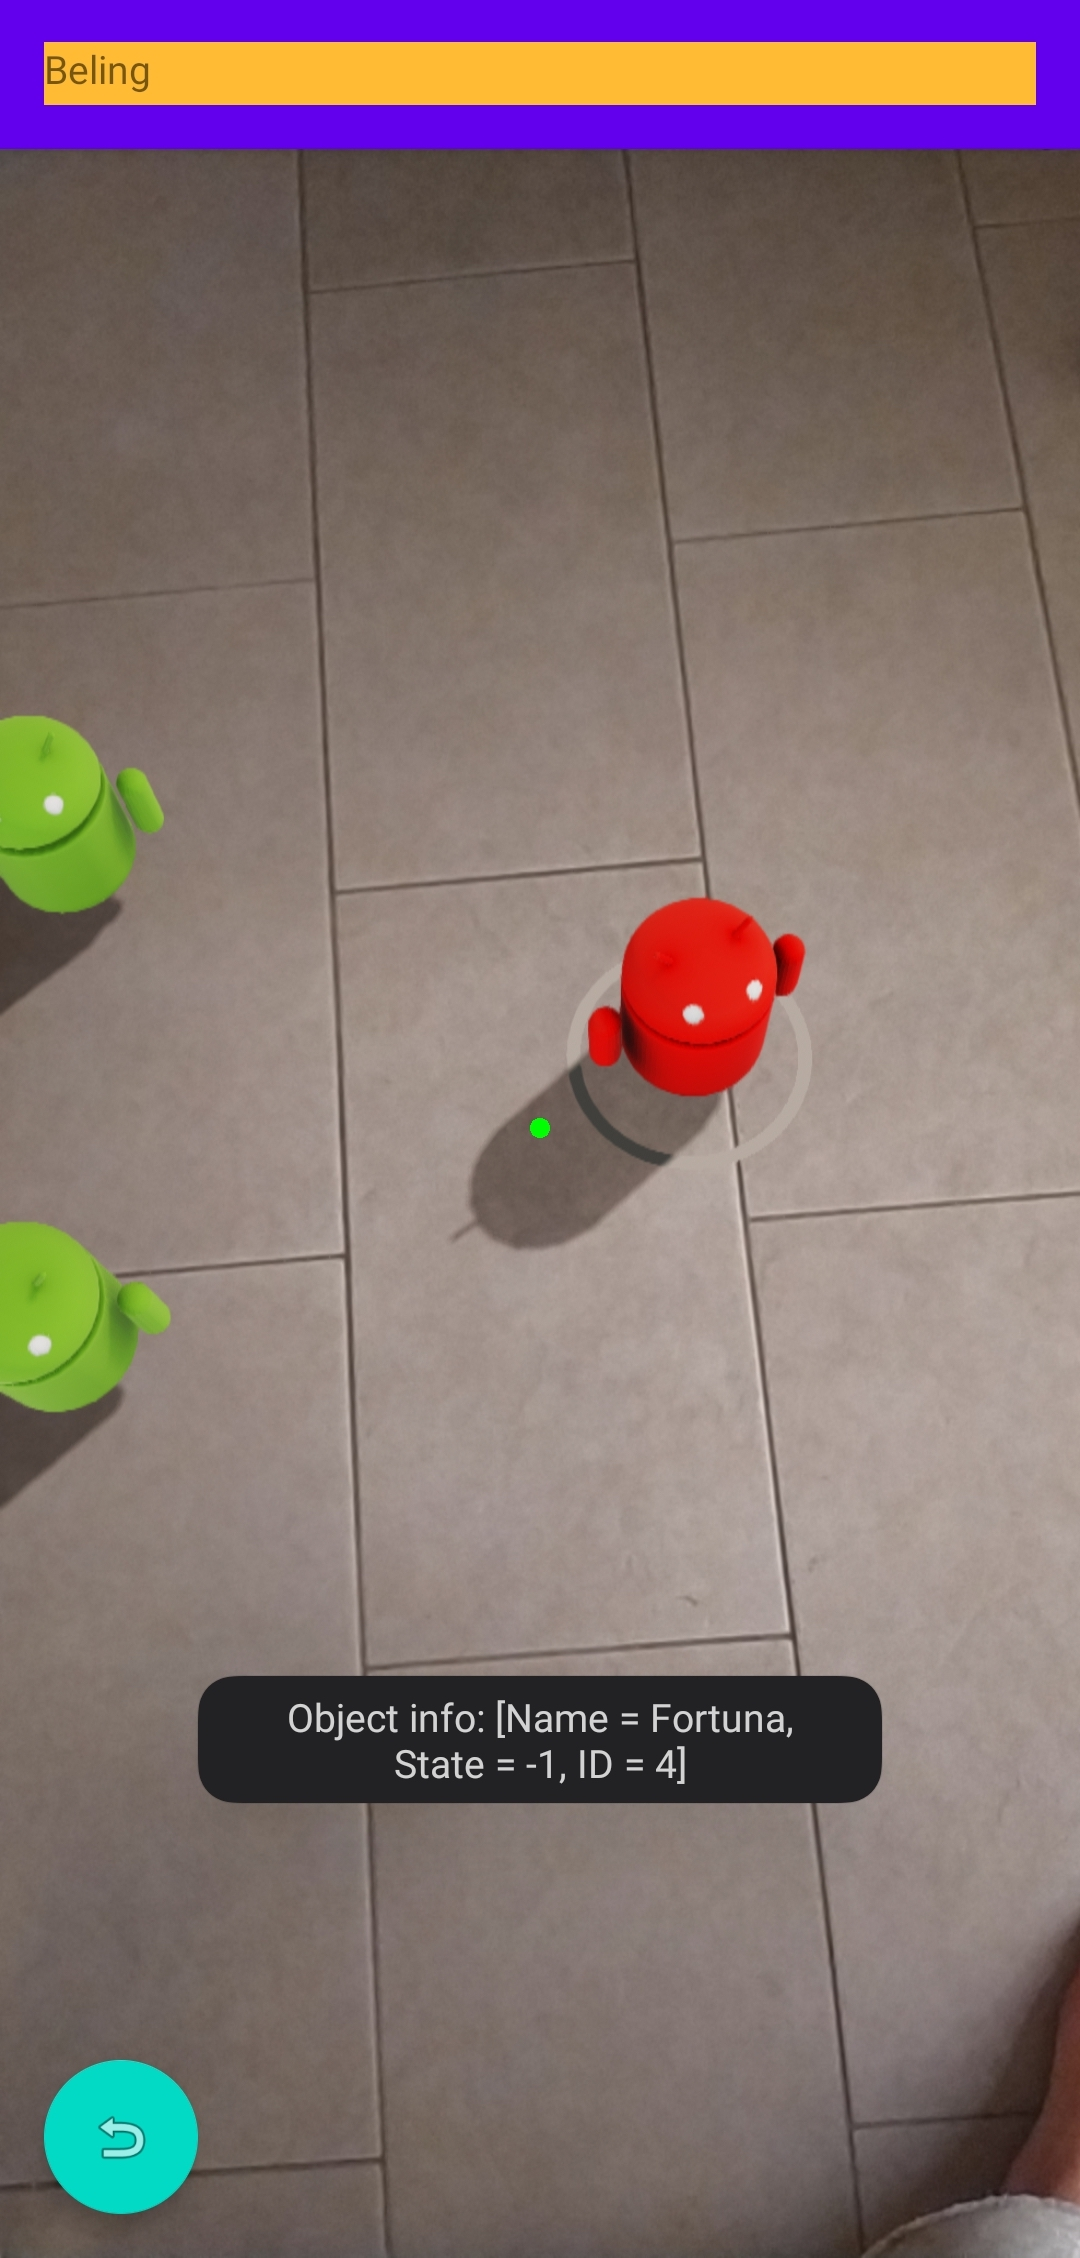
\includegraphics[width=10cm,height=7.5cm,keepaspectratio]{4Umsetzung//Bilder/show_data_to_obj_1.jpg}}
    \subfigure[Anzeige der Objektinformationen 2]{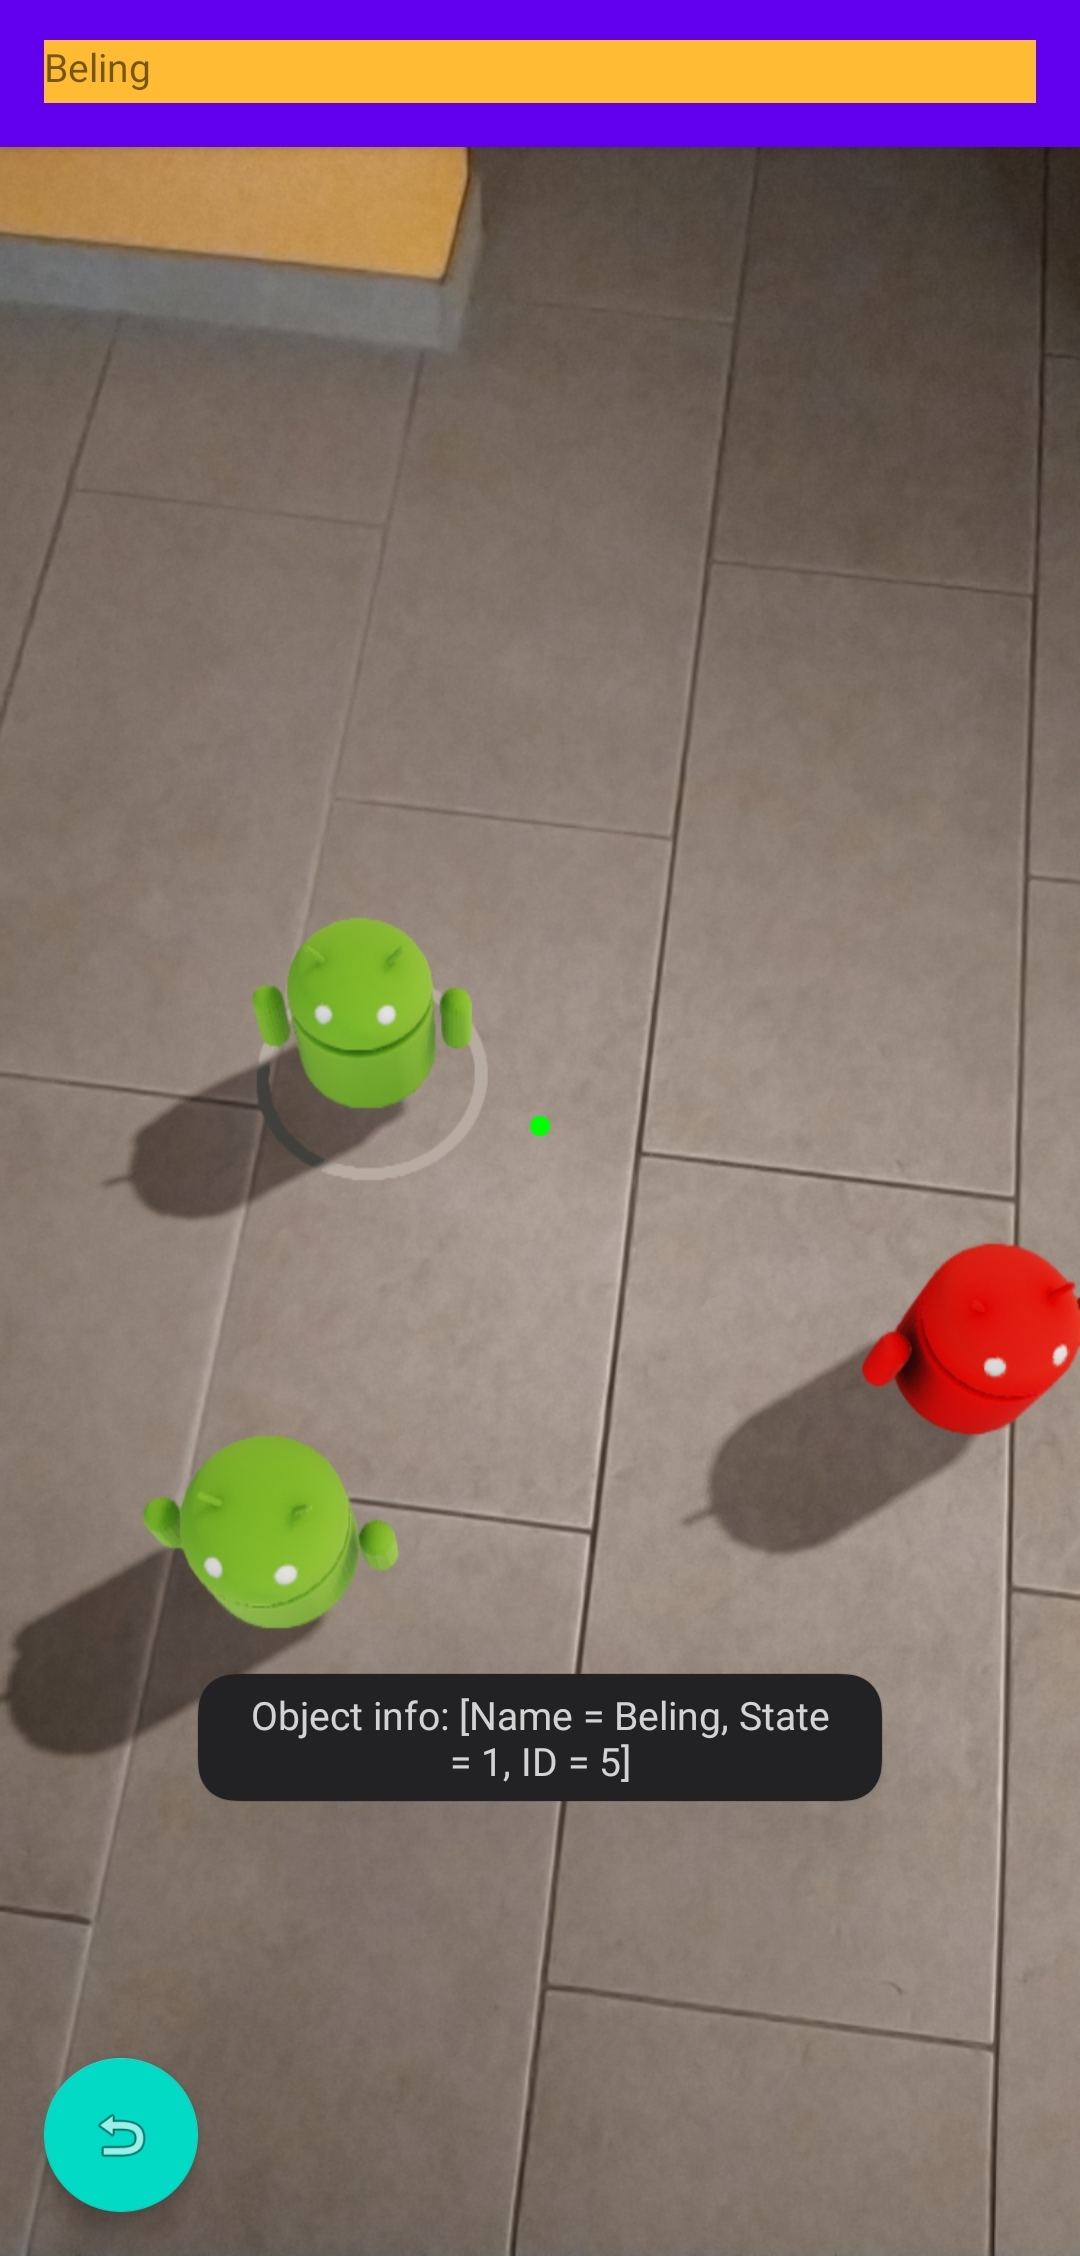
\includegraphics[width=10cm,height=7.5cm,keepaspectratio]{4Umsetzung/Bilder/show_data_to_obj_2.jpg}}
    \subfigure[Anzeige der Objektinformationen 3]{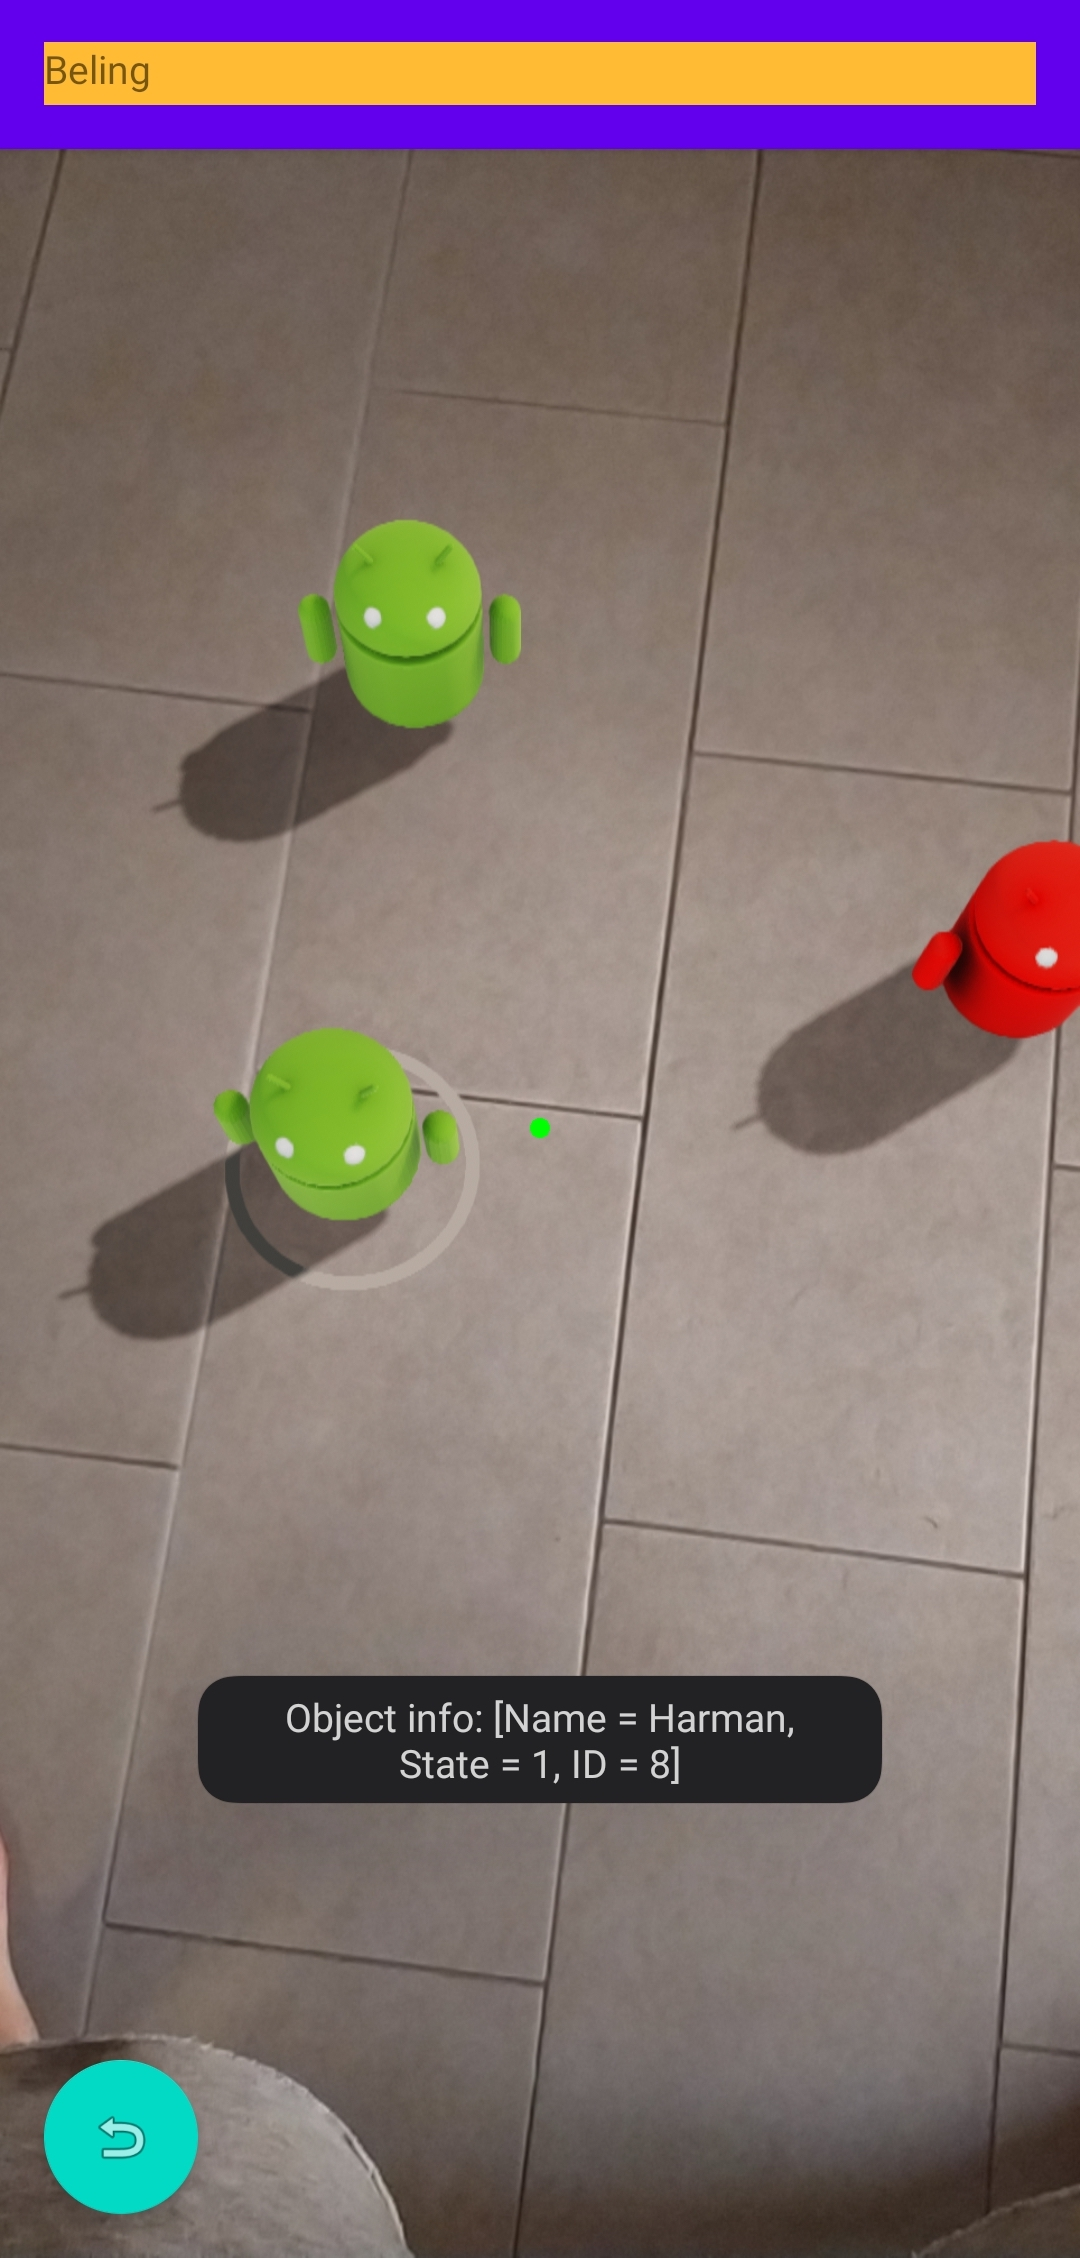
\includegraphics[width=10cm,height=7.5cm,keepaspectratio]{4Umsetzung/Bilder/show_data_to_obj_3.jpg}}
    \caption{Funktion Visualisierungs-Phase Teil 2}
    \label{pic:showdatatoobj}
\end{figure}
\\ 
\linebreak
Nachdem die Aspekte der Front- und Backend-Entwicklung der drei Use Cases geschildert und Einblicke in die Entwicklung und die damit verbundenen Fragestellungen 
und Schwierigkeiten gewährt wurden, geht es nun mit der Evaluierung des Systems, dem Fazit und dem Ausblick weiter.

%werden die implementierten Funktionen anhand eines Testdurchlaufs nochmals genauer 
%dargelegt.
%\section{Testdurchlauf} %/ Test-Szenario
%\label{chap:testdurchlauf}
%Ergänzend zur Implementierung wird in diesem Abschnitt das Resultat und die Anwendung der Applikation anhand eines unabhängigen Tests praktiziert, um die 
%Erzeugnisse der Entwicklung darzustellen und gegebenenfalls erweiternd zur eigentlichen Entwicklungsbeschreibung Ergebnisse zu präsentieren.
\chapter{Evaluation}
\label{chap:Evaluation}
Nach Beendigung der Entwicklungsphase wurde eine Evaluation des Softwareprodukts durchgeführt. Diese dient zur Kategorisierung und Einstufung der Applikation in 
die Gebrauchstauglichkeit. Dabei wurde auch ein Vergleich zu schon bestehenden, bzw. ähnlichen Produkten aufgestellt. Darunter werden 
ebenso Aspekte der Benutzerfreundlichkeit, der Weiterentwicklungsmöglichkeiten beachtet und eine Überprüfung auf gewünschte, bzw. vorab definierte Anforderungen 
und Ziele durchgeführt. 
\\ 
\linebreak
Im Bereich der Industrie gibt es derzeit einige Anwendungen, die auf \acl{AR} aufbauen, allerdings wenige Apps, die sich mit vorliegenden Prozessen 
auseinandersetzen. Es gibt vereinzelt Anwendungen, die auf Interaktionen in Prozessabläufen eingreifen, diese sind allerdings nicht zwangsläufig basierend auf 
einer Smartphone-Applikation. Auch gibt es viele Anwendungsfälle, bei denen auf \acs{VR}- oder \acs{AR}-Brillen vertraut wird. Diese sind meist dafür zuständig, 
Prozesse zu begleiten und zusätzliche Informationen oder Visualisierungen zu projizieren, um dem Nutzer erweiterte Einblicke zu verschaffen. Es gibt auch 
Anwendungen, die visualisierte Arbeitsprozesse vorgeben, um das Potenzial, den Effekt und die Effizienz des „learning by doing“-Ansatzes auszuschöpfen oder auch 
um Vorstellungen und Planungen zu visualisieren, um diese sich besser vorstellen zu können. Beispiel dazu sind zum einen der „augmented presenter“ \cite{tepcon.2020} 
und der „augmented instructor“ \cite{tepcon.2020} der tepcon GmbH. Der „augmented presenter“ bietet die Möglichkeit eine Inneneinrichtung einer Produktionshalle 
zu visualisieren, damit Maschinen an verschiedenen Stellen platziert werden können und anhand dieser Projektion wird überprüft, ob sich die vorgesehene Position 
für die Platzierung der zu planende Maschine eignet. Diese Anwendung dient zur optimierten Fabrikplanung, bevor die Produkte bestellt oder in Betrieb genommen 
werden. Auch kann diese Anwendung für Vertrieb und Marketing, Schulungen und Messen verwendet werden, um die Möglichkeiten der \acs{AR} zu demonstrieren. Der 
„augmented instructor“ basiert auf der Verwendung der \acs{AR}-Brille und visualisiert und projiziert Arbeitsschritte zur Veranschaulichung. 
\\ 
\linebreak
Das entwickelte, prototypische Assistenzsystem dient zur übersichtlichen Veranschaulichung der vorhandenen Maschinen in einer Produktionshalle. Dadurch kann die 
Umgebung eingescannt und Maschinen als Objekte virtuell dargestellt werden. Mit den nötigen Daten ermöglicht dieses System die schnelle und einfache 
Einsicht von Informationen zu einzelnen Maschinen. Auch die Option der Echtzeit-Statusüberprüfung kann in weiterer Entwicklung realisiert werden. 
\\ 
So kann das Assistenzsystem schnell Informationen zur Verfügung stellen, diese dann auch immer verfügbar sind. Durch die einfache Erweiterbarkeit, die 
durch die Architektur gewährleistet ist, können weitere nützliche Funktionen hinzugefügt werden. Demnach wird eine gute Gebrauchstauglichkeit aufgezeigt, die 
stetig erweitert und verbessert werden kann.
\\ 
Auch im Hinblick der Benutzerfreundlichkeit ist eine einfache \acs{UI} gegeben, die überschaubar und schnell zu verstehen ist. Auch nach den Prinzipien der 
Dialoggestaltung der ISO 9241-10 Norm wird eine gute Steuerbarkeit, Selbstbeschreibungsfähigkeit, Individualisierbarkeit und Aufgabenangemessenheit vorgewiesen, 
die durch Usability-Tests in kleinem Rahmen praktiziert wurden. Auf diese in Folgendem nicht näher eingegangen wird. Im Rahmen der Testung wurden 
Verbesserungsvorschläge geäußert, die unter anderem allerdings in diesem Bezug nur an Erweiterungen angeknüpft waren. Ebenso wurde die Genauigkeit bemängelt, da 
diese manchmal fehlerhaft Objekte erstellt und wiedergibt. Diese Ursache ist den Sensoren, je nach Lage und Ausrichtung zuzuschreiben, deshalb ist diese 
Auffälligkeit nur schwer zu umgehend, bzw. zu verhindern. 
\\ 
In der Grundgesamtheit wurde das System als überaus hilfreich eingestuft und mit viel Potenzial bewertet, da in dieser Arbeit lediglich die Konzeption, 
Grundlagenschaffung und prototypische Entwicklung im Fokus stand und so die Grundfunktion implementiert und zur Verfügung gestellt wurde.
\\ 
\linebreak
Nun folgt Abschließend zur Ausarbeitung, um die Dokumentation abzurunden, das allgemeine Fazit des Projekts und der Ausblick, der darlegt wie die Zukunft des 
Projekts aussehen könnte. 

\chapter{Fazit}
\label{chap:Fazit}
Ziel dieser Arbeit war die Konzeption und prototypische Umsetzung eines Assistenzsystems zur Unterstützung industrieller Prozesse. Dabei wurde der Fokus auf die 
übersichtliche und virtuelle Darstellung von Maschinen und Geräten gelegt. Zu der Übersicht kam auch dazu, dass zu einzelnen Objekten schnell Informationen eingesehen 
werden können, um diese bei Bedarf zur Hand zu haben. Dafür wurden in den ersten Schritten Anforderungen zur Umsetzung des Systems festgelegt. Unter Berücksichtigung der 
zu gewährleistenden Modularisierung, damit künftige Weiterentwicklungen an dem Projekt möglich sind und keine großen Herausforderungen darstellt, musste ein geeignetes 
Entwurfsmuster gefunden werden, auf dem die Architektur aufbaut. Durch die Android Architecture Components wurde sich an dem MVVM-Muster angelehnt, welches unter anderem 
die Anforderungen der Modularisierung erfüllt. Bevor die konkrete Umsetzung stattfinden konnte, wurden anhand der Anforderungen und geplanten Funktionen Use Cases für die 
Implementierung definiert. Nachdem diese modelliert waren, konnte das eigentliche System aufgestellt und entwickelt werden.
\\ 
\linebreak
Die Positionsberechnung des Smart-Devices basiert auf Kalkulationen der hardwareinternen Sensoren und unterliegt somit einer sehr sensiblen Basis. Je nach Ausrichtung und 
Lage des Geräts kann sich sowohl dessen Orientierung als auch dessen Blickrichtung unterscheiden und so das eigentliche Ergebnis, obwohl sich das Gerät an der physikalisch 
identischen Position befindet, verfälschen.  

\chapter{Ausblick}
\label{chap:Ausblick}
Der in dieser Arbeit entstandene Prototyp ist ein eigenständiges System zur visualisierten Übersicht von Maschinen und Geräten, beispielsweise in Produktionshallen. 
Bevor die Anwendung allerdings produktiv eingesetzt werden kann, sind noch einige Optimierungen vorzunehmen. Darunter die Verwendung von anderen Objekten 
zur visuellen Darstellung der Maschinen, eventuell auch detailgetreue Abbildungen in einem bestimmten Anwendungsumfeld oder die Verwendung universeller Objekte, die 
ortsunabhängig eingesetzt werden können. Des weiteren die Überarbeitung der Informationsanzeige der Objekte, die aktuell über ein vereinfachtes Informationsfenster 
eingeblendet werden. Eine weitere \acl{AR} basierte Anzeige der Informationen wäre dabei denkbar. In dieser Arbeit wurden lediglich die Grundsteine für ein Projekt 
gelegt, welches in Zukunft stetig weiterentwickelt werden kann und viel Potential für weitere Funktionen, auf Basis der \acs{AR}-Anwendung, bietet. Die Ergebnisse 
des Prototypen sind für erste Tests gut, allerdings für den eigentlichen Einsatz noch nicht geeignet, da noch kein erwähnenswerter Mehrwert daraus resultiert und die 
Maschinenbezogenen Daten im Hinblick auf die statusabhängigen Informationen keine Echtzeit-Auskünfte bietet. Diese können daher aktuell nur provisorisch beschrieben 
werden. Daher muss der Prototyp weiterentwickelt und verbessert werden. 
\\ 
\linebreak
Um Informationen über einzelne Maschinen in Echtzeit aufrufen und visualisieren zu können, wäre ein weiterer Entwicklungsschritt die Benutzung von Echtzeitdaten der 
Maschinen. Dafür wäre eine Datenaufbereitung und eine globale Verfügbarkeit der Informationen notwendig. Diese Idee könnte über eine \acl{IoT}-Lösung umgesetzt werden. 
Dabei könnten die Maschinendaten, die über eine Cloud ausgelagert sind, in Echtzeit abgegriffen und stets den aktuellen Zustand und Status der einzelnen Geräte 
abgerufen werden. Auch könnten die Daten direkt von den jeweiligen Geräten verwendet, aufbereitet und in der Anwendung genutzt werden. Dadurch wäre die genauer 
Informationsgebung zu den Objekten möglich.
\\ 
\linebreak
Eine zusätzlicher Erweiterung der Anwendung wäre das automatische lokalisieren von Anomalien sämtlicher Maschinen. Dabei würden auftretende Fehler registriert werden 
und über eine Benachrichtigung den Nutzer darüber in Kenntnis setzen. Somit könnte bei Ausfällen der Maschinen schnell reagiert und agiert werden, um diese auftretenden 
Fehler schnellstmöglich zu beheben. 
\\ 
Basierend auf dieser Erweiterung wäre es ebenso möglich bei großen Umgebungen, bzw. Produktionshallen eine räumliche Navigation einzubauen, die den Mechaniker auf 
schnellstem Wege zu der wartungsbedürftigen Maschine zu leiten, um eine Orientierung in der Räumlichkeit zu gewährleisten. 
\\ 
\linebreak
Derzeit steht nur eine Laufzeitumgebung für ein natives Android System zur Verfügung. Ein weiterer Schritt zur Systemoptimierung wäre die Einbindung von \acs{AR}-Brillen, 
im Vergleich zum Smartphone wäre der Nutzer in seinen Bewegungen uneingeschränkt und könnte sich mit den Händen frei bewegen. 
\\ 
Aufbauend darauf könnten auch Arbeitsschritte der Reparaturarbeiten optimiert werden, indem über die \acs{AR}-Brille Reparaturschritte und Anleitungen zur Wartung der 
Maschine bereitgestellt werden. 
\\ 
\linebreak
Dies sind einige Ansätze, mit denen die Einsatzmöglichkeiten des Projekts in Zukunft erweitert werden könnten, um ein umfängliches Assistenzsystem zu erschaffen und einen 
echten Mehrwert in unterstützenden, industriellen Maßnahmen zu gewährleisten.  




% Ab hier beginnt der Anhang
\appendix
\addcontentsline{toc}{chapter}{Anhang}

\addcontentsline{toc}{chapter}{Index}
\printindex

\addcontentsline{toc}{chapter}{Literaturverzeichnis}

% Haben Sie das "biblatex"-Paket nicht installiert, benutzen Sie folgendes:
% Ohne das "biblatex"-Paket (s. bericht.sty) produziert folgendes
% "deutsche" Zitate in Literaturverzeichnissen gemaß der Norm DIN 1505,
% Teil 2 vom Jan. 1984.
% Die Zitatmarken werden alphabetisch nach Verfassern
% sortiert und sind durch abgekürzte Verfasserbuchstaben plus
% Erscheinungsjahr in eckigen Klammern gekennzeichnet.

% \bibliographystyle{alphadin}
% \bibliography{bericht}

%%%%%%%%%%%%%%%%%%%%%%%%%%%%%%%%%%%%%%%5
% BIBLATEX
% Benutzt man das "biblatex"-Paket, muß man folgendes schreiben:
\def\refname{Literaturverzeichnis}
\printbibliography
%%%%%%%%%%%%%%%%%%%%%%%%%%%%%%%%%%%%%%%5
%%%%%%%%%%%%%%%%%%%%%%%%%%%%%%%%%%%%%%%


%\newpage
%\addcontentsline{toc}{chapter}{Liste der ToDo's}
%\listoftodos[Liste der ToDo's]


\end{document}